% ===========================================================================
% BRCA Multi-Omics Data Mining — Academic Paper
% Version: 0518-1115
% Compile: xelatex -> biber -> xelatex -> xelatex
% ===========================================================================
\documentclass[12pt,a4paper]{ctexart}

% ---------- Packages ----------
\usepackage[top=2.5cm, bottom=2.5cm, left=3cm, right=2.5cm]{geometry}
\usepackage{graphicx}
\usepackage{booktabs}
\usepackage[labelfont=bf,font=small]{caption}
\usepackage[hidelinks]{hyperref}
\usepackage{amsmath}
\usepackage{float}
\usepackage{array}
\usepackage{multirow}
\usepackage{listings}
\usepackage{xcolor}

\lstset{
  basicstyle=\ttfamily\footnotesize,
  breaklines=true,
  frame=single,
  numbers=left,
  numberstyle=\tiny,
  backgroundcolor=\color{gray!5}
}

% ---------- Bibliography: GB/T 7714-2015 ----------
\usepackage[backend=biber,style=gb7714-2015]{biblatex}
\addbibresource{references.bib}

\graphicspath{{../../results/figures_pub/}}

\title{\heiti\zihao{3} 基于多组学数据挖掘的乳腺癌分子特征分析}
\author{}
\date{}

\begin{document}

\maketitle

% ==================== 摘要 ====================
\begin{abstract}
\noindent
乳腺癌是全球发病率最高的恶性肿瘤，其分子异质性是精准诊疗面临的核心挑战。本研究基于TCGA-BRCA多组学数据（mRNA转录组25,981个基因、miRNA表达谱1,881个、体细胞突变15,413个基因及临床注释94项），对1,076例多组学共同患者进行了系统性的数据挖掘分析。研究综合运用DESeq2差异表达分析、LASSO和随机森林分类、PCA/t-SNE聚类、WGCNA共表达网络、Cox比例风险回归、maftools突变景观分析、g:Profiler功能富集分析、arules关联规则挖掘及ConsensusClusterPlus共识聚类等算法。主要结果包括：鉴定6,768个显著差异表达基因（$|\log_2\text{FC}|>1$, FDR$<0.05$），其中上调4,334个、下调2,434个；LASSO分类器以89.4\%准确率实现三分类分子亚型预测，仅使用35个基因；WGCNA识别9个共表达模块，blue模块枢纽基因模块隶属度达0.959；Cox模型C-index为0.771，Stage IV风险比达8.74；PIK3CA（37.3\%）和TP53（35.2\%）为最高频突变基因；功能富集揭示上调基因显著富集于细胞周期通路（Reactome Cell Cycle, 187个基因, $p=1.5\times10^{-21}$）。本研究为乳腺癌多组学数据挖掘提供了完整分析框架。

\vspace{1em}
\noindent\textbf{关键词}：乳腺癌；TCGA；多组学数据挖掘；差异表达分析；WGCNA；预后模型
\end{abstract}

\newpage

% ==================== 1 引言 ====================
\section{引言}

\subsection{研究背景}

据国际癌症研究机构（IARC）GLOBOCAN 2022统计，全球每年新发癌症约2,000万例，死亡约970万例\cite{sung2024global}。其中女性乳腺癌以约230万例新发病例居全球恶性肿瘤发病率首位，同年导致约67万例死亡。在中国，乳腺癌的发病率和死亡率持续上升，且发病年龄显著早于欧美国家。

乳腺癌的发生发展涉及多基因突变累积、表观遗传重塑及信号通路交互失调等复杂的分子过程\cite{hanahan2011hallmarks}。传统单一维度研究方法难以全面揭示乳腺癌的系统性分子特征。以癌症基因组图谱（The Cancer Genome Atlas, TCGA）\cite{tcga2012comprehensive}为代表的国际大型合作项目提供了涵盖多组学的海量公开数据。在此背景下，数据挖掘技术为从高维度组学数据中提取具有生物学和临床价值的信息提供了方法论支撑。

\subsection{乳腺癌分子分型}

乳腺癌是由多种分子特征各异的亚型构成的异质性疾病集合。Perou等\cite{perou2000molecular}于2000年首次提出乳腺癌分子分型体系，目前广泛认可的固有分子亚型包括四类：Luminal A型（50\%--60\%，ER+/PR+/HER2-/Ki-67低表达），Luminal B型（15\%--20\%），HER2过表达型（10\%--15\%），三阴性型（15\%--20\%）。尽管该体系已广泛用于临床，同一亚型内部的生物学异质性仍然显著，整合多组学数据进一步挖掘分子分型的内在结构具有重要的研究价值。

\subsection{数据挖掘在癌症研究中的应用}

在差异表达分析方面，DESeq2\cite{love2014moderated}基于负二项分布对RNA-seq计数数据建模。WGCNA\cite{langfelder2008wgcna}通过构建无标度拓扑网络将基因聚类为共表达模块。LASSO-Cox\cite{simon2011regularization}能有效应对高维数据中的维数灾难。g:Profiler\cite{kolberg2023gprofiler}提供一站式多数据库功能富集。Apriori算法\cite{agrawal1994fast}可从离散化数据中挖掘关联规则。共识聚类\cite{wilkerson2010consensus}通过重采样评估聚类稳定性。

\subsection{研究目的与论文结构}

本研究以TCGA-BRCA多组学数据为对象，综合运用多种数据挖掘方法，系统分析乳腺癌的分子特征。论文结构如下：第2章介绍材料与方法；第3章呈现分析结果；第4章为讨论；第5章给出结论；附录提供核心R代码。

% ==================== 2 材料与方法 ====================
\section{材料与方法}

\subsection{数据来源}

本研究数据来源于TCGA-BRCA队列。所有数据通过TCGAbiolinks R包\cite{colaprico2016tcgabiolinks}从GDC API获取（GDC Data Release 42.0），涵盖四个数据层：
（1）mRNA转录组（HiSeq RNA-seq, STAR-Counts流程）：原始计数矩阵包含60,660个基因；
（2）miRNA转录组（HiSeq miRNA-seq, BCGSC miRNA Profiling）：1,881个miRNA；
（3）体细胞突变（WES, MuTect2流程）：MAF格式突变注释文件；
（4）临床信息：94个原始变量。

\subsection{数据预处理}

\textbf{mRNA数据预处理}：低表达过滤标准为至少在10\%样本中counts $\geq$ 10，保留25,981个基因（42.8\%）。采用TPM归一化，基因标识符通过org.Hs.eg.db建立Ensembl ID到Gene Symbol的映射。临床数据提取25个核心变量，分子亚型根据ER/PR/HER2免疫组化状态分类。缺失值：数值型采用中位数填补，分类型采用众数填补。miRNA数据全部保留，突变数据经maftools\cite{mayakonda2018maftools}加载和质控。

\textbf{多组学整合}：提取各数据层样本条形码前12个字符作为患者ID，取交集确定1,076例核心患者队列。

\subsection{分析方法}

\textbf{差异表达分析}：采用DESeq2\cite{love2014moderated}进行肿瘤vs正常（$n=1,105$, $n=113$）和TN vs Luminal A（$n=115$, $n=950$）的差异表达分析，阈值FDR $<0.05$且$|\log_2\text{FC}|>1$。

\textbf{功能富集分析}：采用g:Profiler（gprofiler2 R包）\cite{kolberg2023gprofiler}，覆盖GO:BP、GO:MF、GO:CC、KEGG、Reactome和WikiPathway（FDR $<0.05$，排除IEA）。

\textbf{分类}：LASSO（5折交叉验证，$\alpha=1$）、随机森林（ntree=500）、XGBoost（nrounds=100）。输入为Top 500可变基因$\log_2(\text{TPM}+1)$，7:3分层划分。

\textbf{聚类}：PCA（Top 2,000基因中心化标准化）、t-SNE（perplexity=30）、K-means（$K=2$--10，轮廓系数）、共识聚类（80\%重采样，1,000次迭代）\cite{wilkerson2010consensus}。

\textbf{WGCNA}\cite{langfelder2008wgcna}：Top 5,000可变基因，signed网络，minModuleSize=30，mergeCutHeight=0.25。

\textbf{生存分析}：Kaplan-Meier（log-rank）、多变量Cox（C-index、似然比检验）、3年生存列线图（rms包）。

\textbf{突变分析}：maftools\cite{mayakonda2018maftools}，TMB按每兆碱基计算（WES $\approx$38 Mb）。

\textbf{关联规则}：Apriori（支持度0.3，置信度0.7）。miRNA-mRNA网络：Pearson相关（$|r|>0.4$）。

\subsection{分析环境}

R 4.6.0 + Bioconductor 3.23，Windows 11。主要R包：DESeq2、gprofiler2、caret、randomForest、glmnet、WGCNA、survival、survminer、rms、maftools、arules、ConsensusClusterPlus、ggplot2、ggsci、pheatmap。论文编译：MiKTeX 25.12 + XeLaTeX。

% ==================== 3 结果 ====================
\section{结果}

\subsection{数据概览}

经预处理和跨组学整合，最终分析数据集概况见表\ref{tab:data}。mRNA覆盖1,094例肿瘤（另113例正常），miRNA覆盖1,079例。多组学对齐后获得1,076例共同患者（重叠率98.4\%），突变数据覆盖990例（983例患者）。临床特征中Luminal A占绝对优势（950例，86.3\%），HER2-enriched仅37例（3.4\%），Triple Negative 115例（10.4\%）；Stage II占比最高（58.9\%），Stage IV仅20例（1.8\%），反映了乳腺癌以早中期诊断为主的临床实际。中位OS随访约2.7年，死亡事件87例（7.9\%），事件率偏低是后续预后模型构建面临的核心约束。

\begin{table}[H]
\centering
\caption{多组学数据集总览}
\label{tab:data}
\begin{tabular}{llll}
\toprule
数据层 & 平台 & 特征数 & 样本量 \\
\midrule
mRNA表达 & HiSeq RNA-seq & 25,981 genes & 1,094 + 113 normal \\
miRNA表达 & HiSeq miRNA-seq & 1,881 miRNAs & 1,079 \\
体细胞突变 & WES (MuTect2) & 15,413 genes & 990 \\
临床数据 & TCGA Clinical & 25 variables & 1,174 \\
\bottomrule
\end{tabular}
\end{table}

\subsection{差异表达与功能富集}

\subsubsection{Tumor vs Normal 差异表达}

DESeq2在肿瘤（$n=1,105$）与正常（$n=113$）组织间共鉴定6,768个显著差异表达基因（$|\log_2\text{FC}|>1$, FDR$<0.05$），其中肿瘤相对正常上调4,334个、下调2,434个（表\ref{tab:deg}）。上调基因数量为下调的1.78倍，提示肿瘤细胞中转录激活事件的广泛性——已知癌症转录组以代谢重编程、细胞周期激活和增殖信号增强为特征，上调偏倚与这些过程的全局性激活一致。

图\ref{fig:volcano}以火山图形式展示了全部25,981个基因的分布格局。上调侧（$\log_2\text{FC}>0$）横坐标在2--5范围内的基因密度远高于下调侧（$\log_2\text{FC}<0$）对称位置。分布在图的远右侧（$\log_2\text{FC}>4$）且$-\log_{10}(p)>20$的极端离群基因代表在肿瘤中高度过表达且统计学证据极强的候选生物标志物。图中标注了差异最显著的若干基因的Gene Symbol，使读者可直接识别极端位点对应的基因身份。两条虚线分别标记了$|\log_2\text{FC}|=1$（2倍变化）和$p=0.05$的显著性阈值——分布于图右上和左上象限的基因即为纳入后续分析的显著差异表达基因集合。

\begin{figure}[H]
\centering
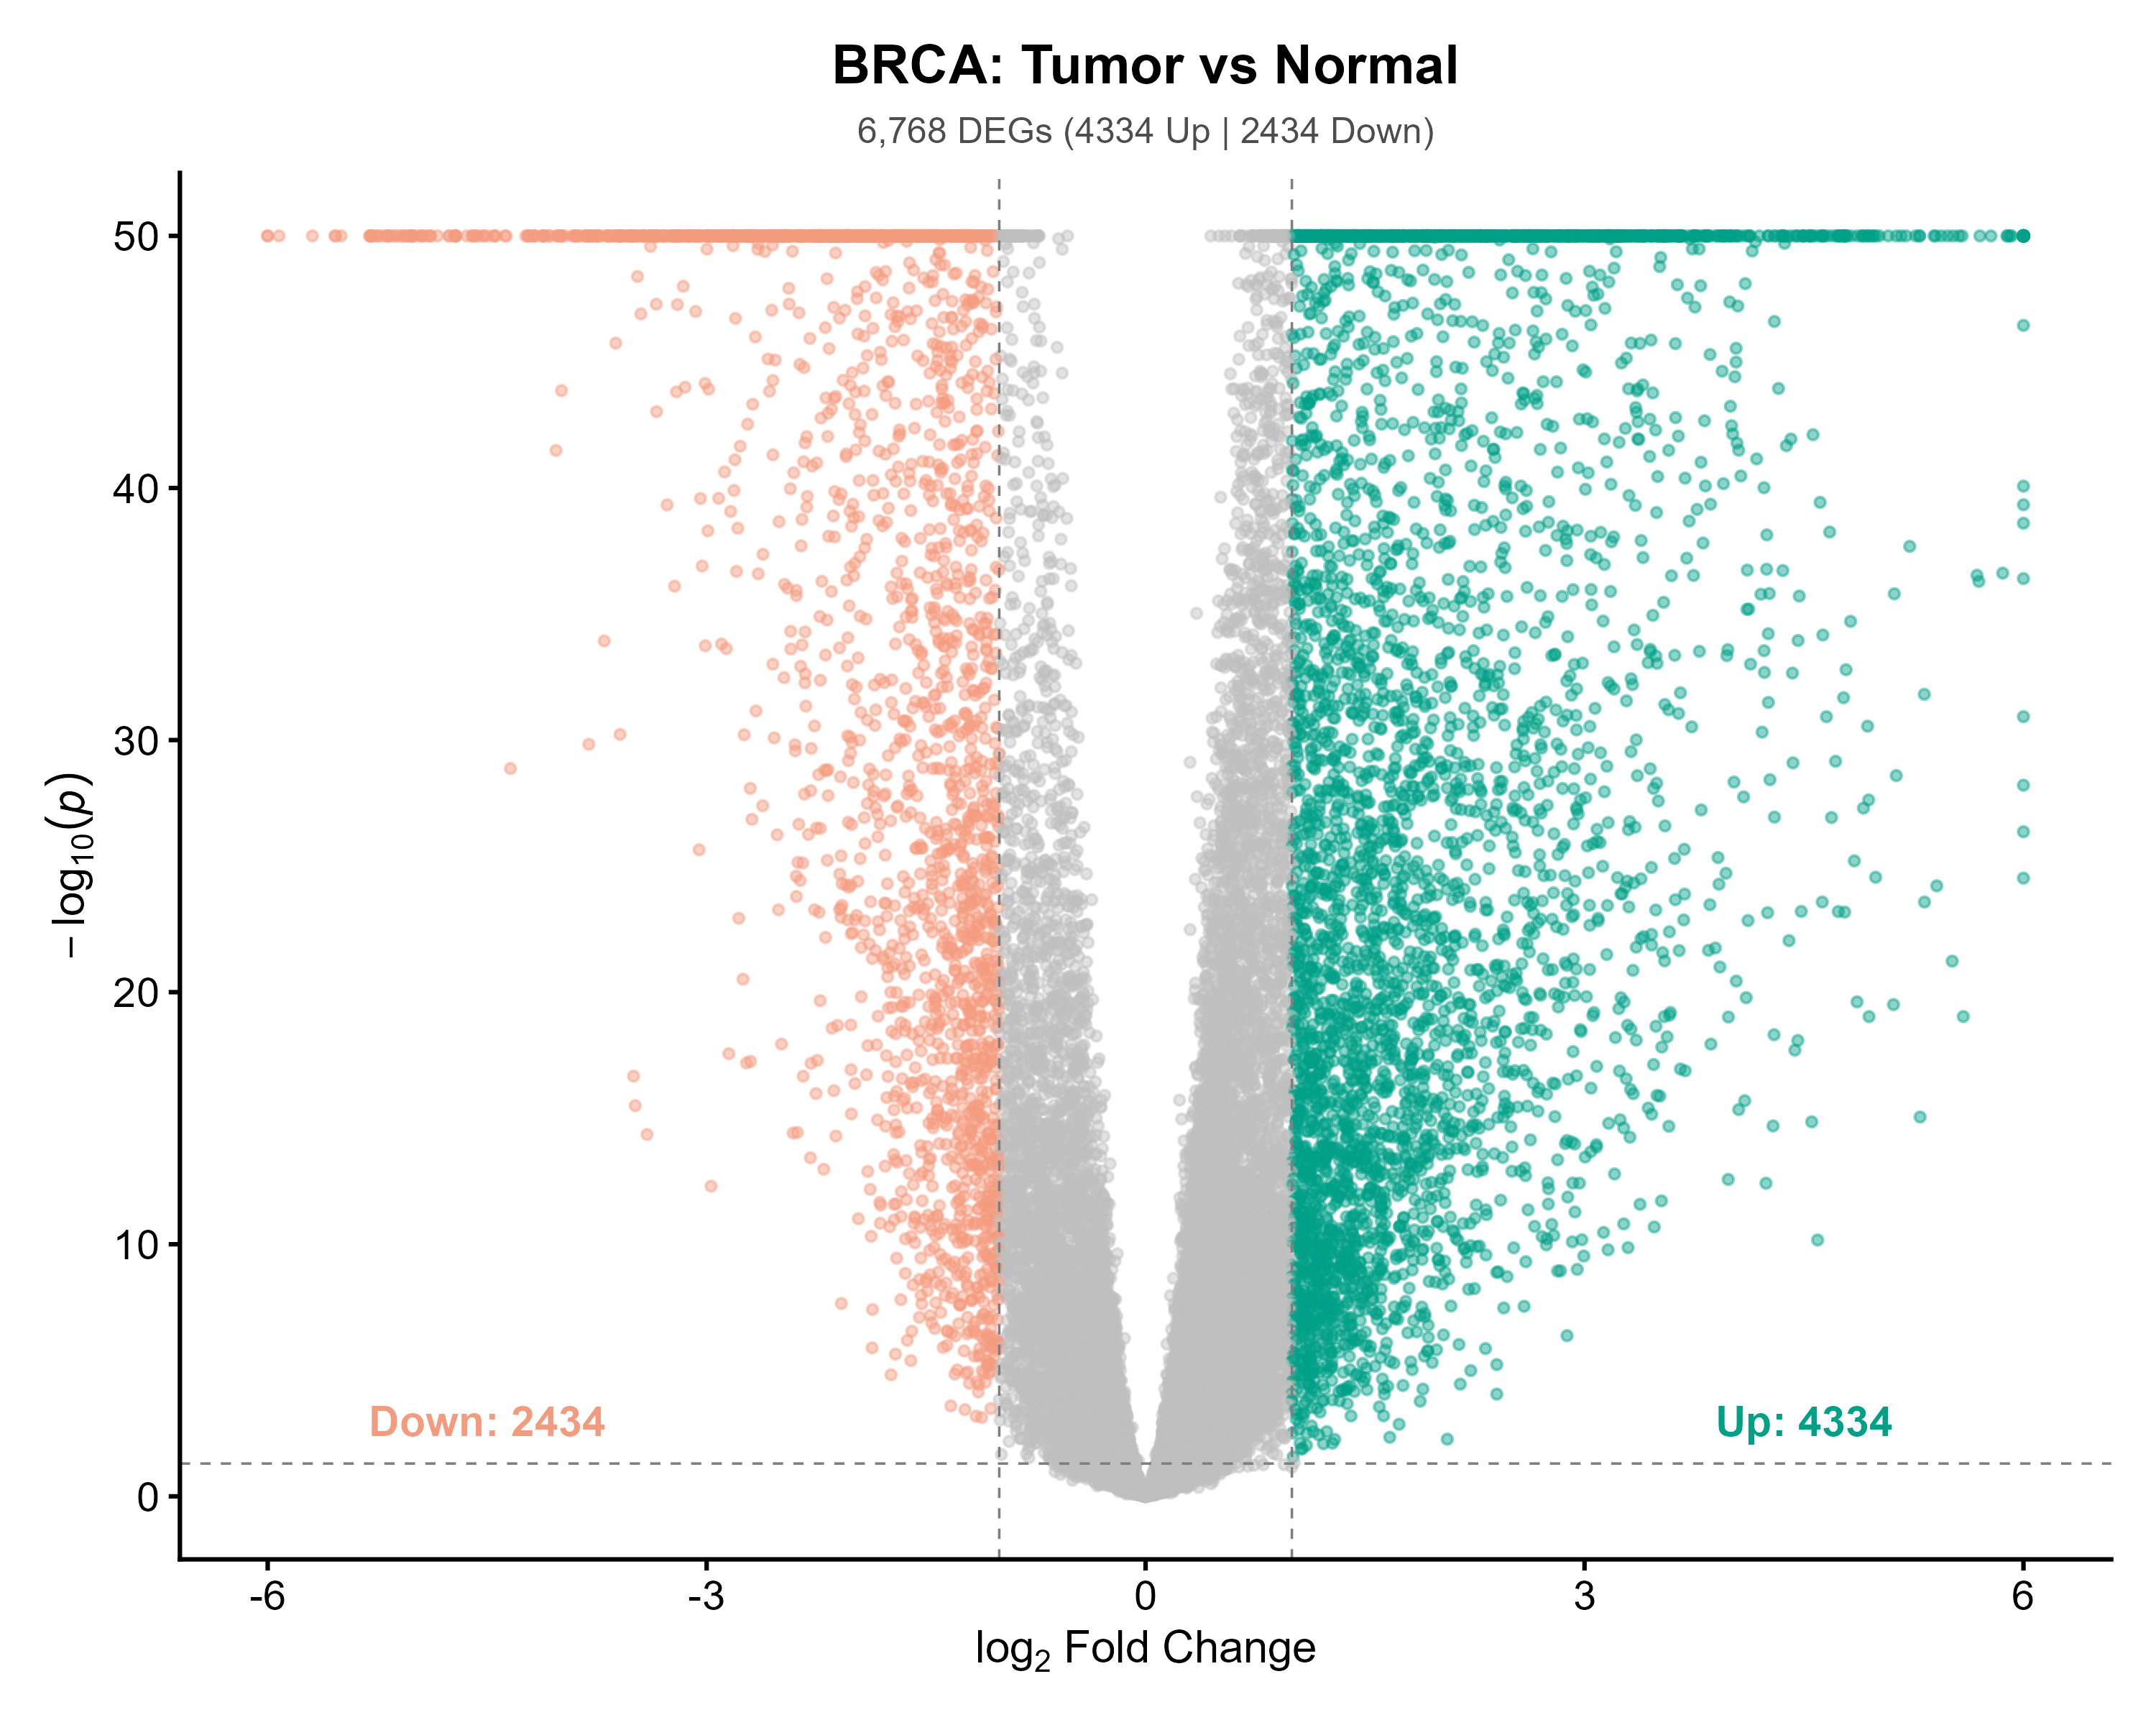
\includegraphics[width=0.85\textwidth]{fig1_volcano.png}
\caption{差异表达火山图。横轴为$\log_2$ Fold Change（截断$\pm6$），纵轴为$-\log_{10}(p)$（截断50）。红色=上调（4,334个），蓝色=下调（2,434个），灰色=不显著。两条虚线分别标记$|\log_2\text{FC}|=1$和$p=0.05$的阈值。ggrepel标注了差异最显著的前10个上调基因和前10个下调基因的Gene Symbol。}
\label{fig:volcano}
\end{figure}

\begin{table}[H]
\centering
\caption{差异表达分析结果}
\label{tab:deg}
\begin{tabular}{ll}
\toprule
指标 & 数值 \\
\midrule
总DEGs（$|\log_2\text{FC}|>1$, FDR$<0.05$） & 6,768 \\
上调基因数 & 4,334 \\
下调基因数 & 2,434 \\
分析方法 & DESeq2 (Wald test, BH correction) \\
\bottomrule
\end{tabular}
\end{table}

\subsubsection{亚型间差异表达}

Triple Negative（$n=115$）与Luminal A（$n=950$）之间的差异表达分析鉴定出4,888个显著基因（$|\log_2\text{FC}|>1$, FDR$<0.05$），其中TN上调2,270个，Luminal A上调2,618个（图\ref{fig:tnla}）。这一数字与Tumor vs Normal差异基因总数（6,768）处于同一数量级，说明两种极端分子亚型之间的转录组差异幅度不亚于肿瘤与正常组织的差异——这是一个非平凡的发现：它表明在乳腺癌内部，不同亚型代表了本质上不同的转录组状态，而非同一状态的细微调变。在TN中高表达的基因可优先作为TNBC潜在治疗靶点的候选来源。

\begin{figure}[H]
\centering
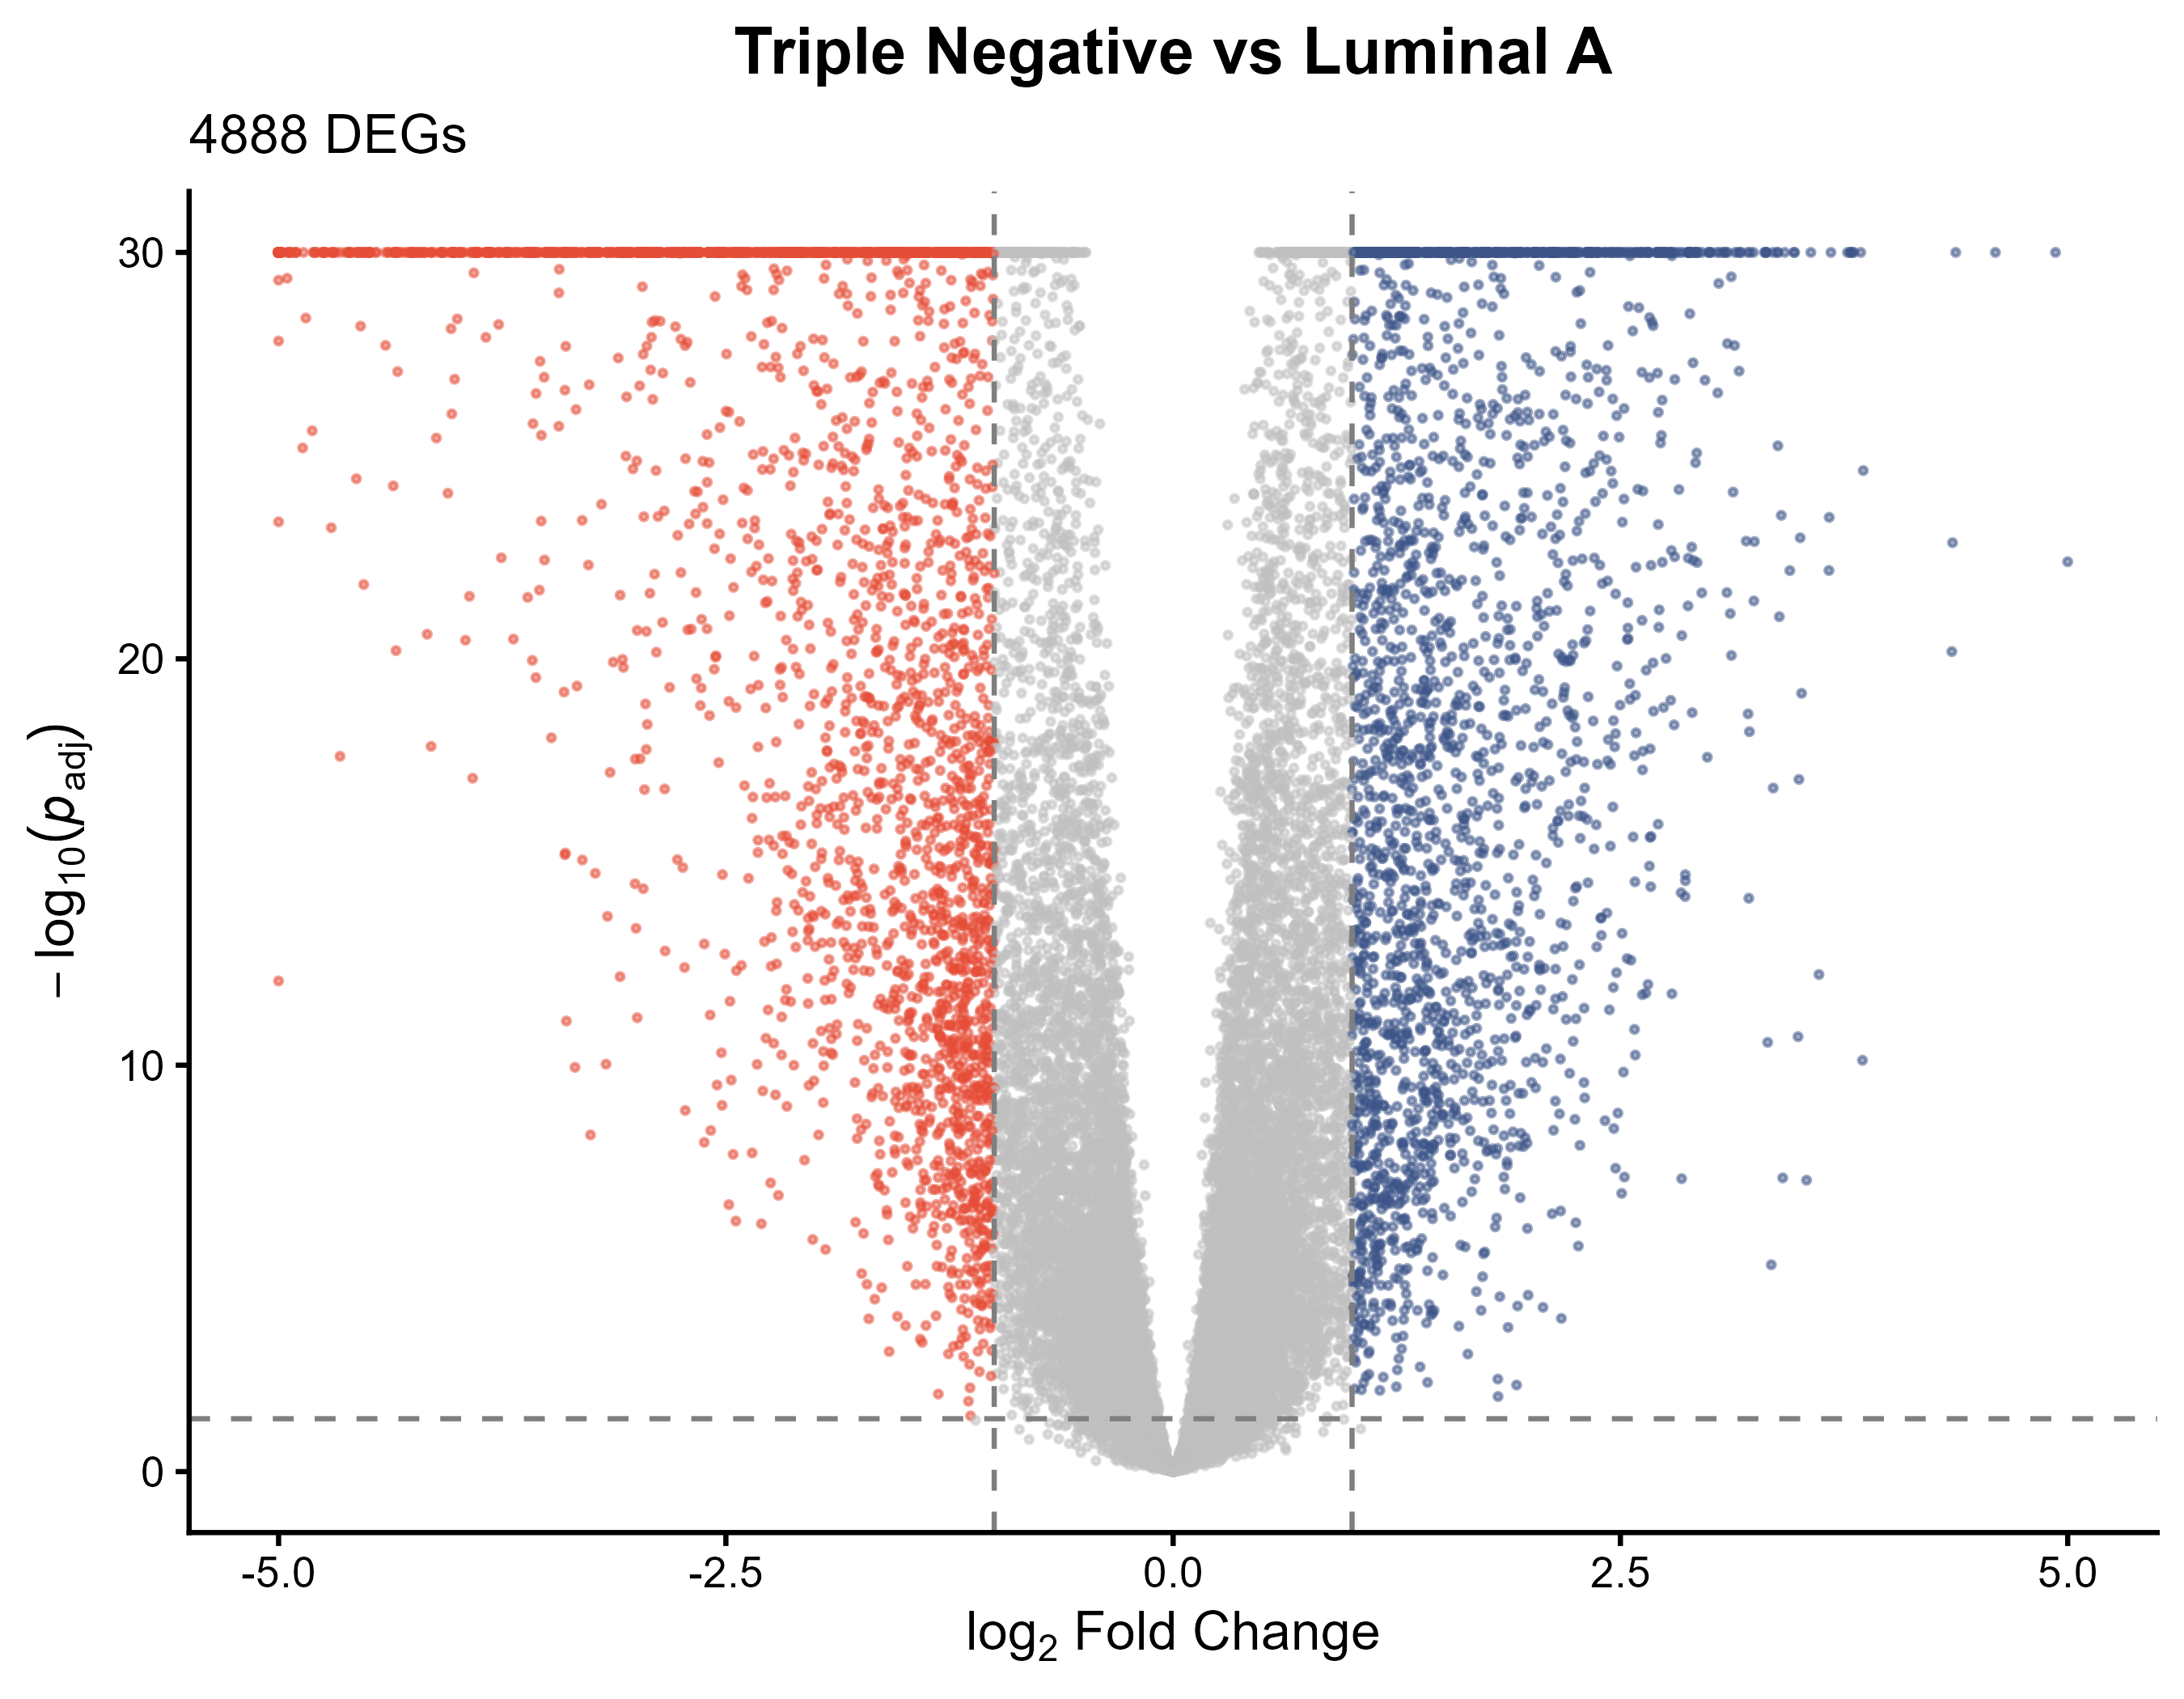
\includegraphics[width=0.85\textwidth]{fig17_tn_vs_la_volcano.png}
\caption{TN vs Luminal A差异表达火山图。横轴为$\log_2$ Fold Change（截断$\pm5$），红色=TN中上调（2,270个），绿色=Luminal A中上调（2,618个）。TN上调基因构成TNBC特异性靶点的候选集。}
\label{fig:tnla}
\end{figure}

\subsubsection{功能富集分析}

上调基因的富集信号呈现高度集中的特征（图\ref{fig:enrich_up}）。在643条显著条目（FDR$<0.05$）中，前五位全部来自Reactome数据库，且功能主题高度一致：Cell Cycle（187个基因，$p=1.5\times10^{-21}$）以压倒性的显著性居首，其后依次为Cell Cycle Mitotic（160个基因）、Nucleosome Assembly、DNA Replication和Mitotic Chromosome Condensation。这五个通路共同指向一个核心生物学结论：BRCA肿瘤中转录激活最剧烈的事件是DNA复制和染色体分离机器。187个上调基因共同参与Cell Cycle通路，这一交叠规模在所有显著条目中最大，反映细胞周期调控在BRCA转录组全局失调中的核心地位。同时需注意到上调条目主要来源于Reactome（占绝对多数），其次为GO:BP和KEGG——这一分布特征与该通路类别的注释覆盖度有关，Reactome在细胞周期调控方面有更为细致的层级化注释。

下调基因的富集方向截然不同（图\ref{fig:enrich_down}）。1,414条显著条目（数量为上调的两倍以上）分布更为广泛，主要集中于细胞外基质组织（ECM organization）、细胞黏附（Cell adhesion）、脂质代谢及PI3K-Akt信号通路。下调基因中ECM-receptor interaction和Focal adhesion两条通路的显著性突出。从肿瘤生物学的角度解读：肿瘤细胞要获得侵袭和转移能力，需要部分摆脱对细胞外基质的结构依赖，下调黏附和ECM组织相关基因是这一转变的分子基础。下调条目数量远超上调（1,414 vs 643），暗示被抑制的生物学功能类别比被激活的更为分散——这可能反映了肿瘤为存活需要在多种正常功能上妥协的生物学现实。表\ref{tab:enrich}汇总了三组基因集的富集统计。

\begin{figure}[H]
\centering
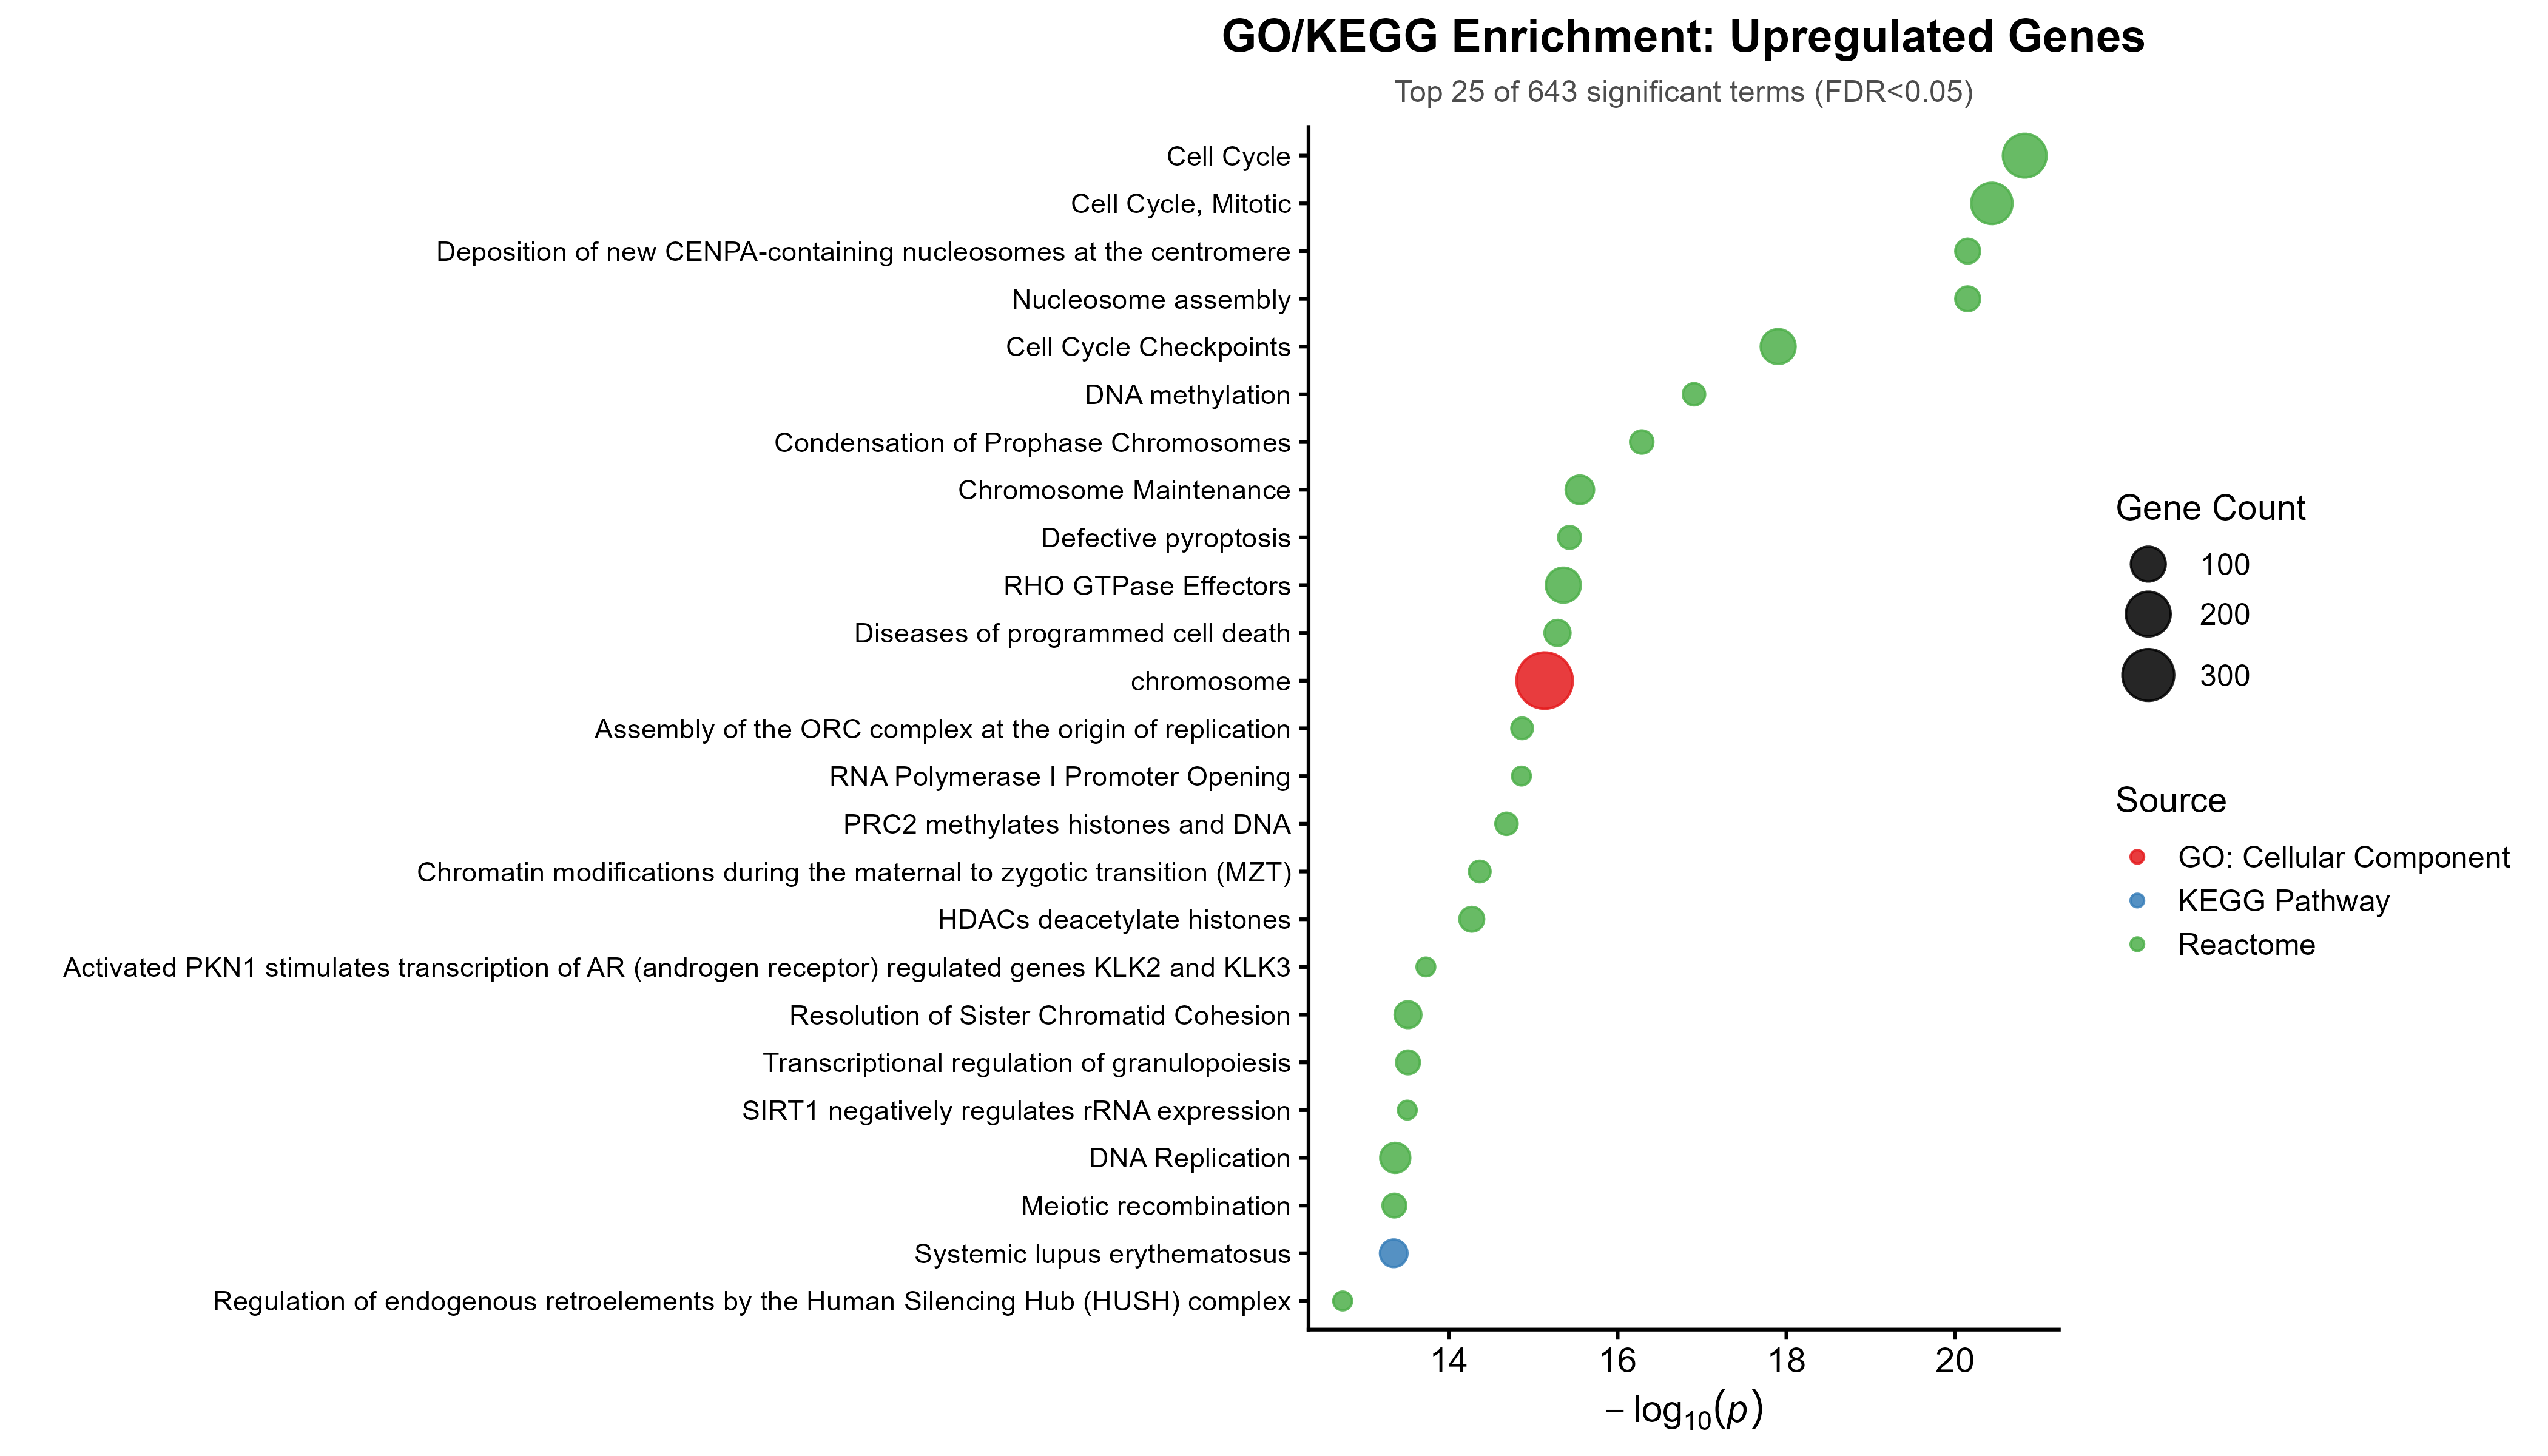
\includegraphics[width=0.85\textwidth]{fig12_enrichment_up.png}
\caption{上调基因GO/KEGG/Reactome富集气泡图（Top 25, FDR$<0.05$）。横轴为$-\log_{10}(p)$值，纵轴为通路名称按显著性降序排列。气泡大小表示交叠基因数量（最大为Cell Cycle的187个基因），颜色区分来源数据库（GO:BP、GO:MF、GO:CC为红/橙/绿色系, KEGG为紫色, Reactome为蓝色, WikiPathway为粉色）。前五位全部来自Reactome，功能主题高度集中于细胞周期调控。}
\label{fig:enrich_up}
\end{figure}

\begin{figure}[H]
\centering
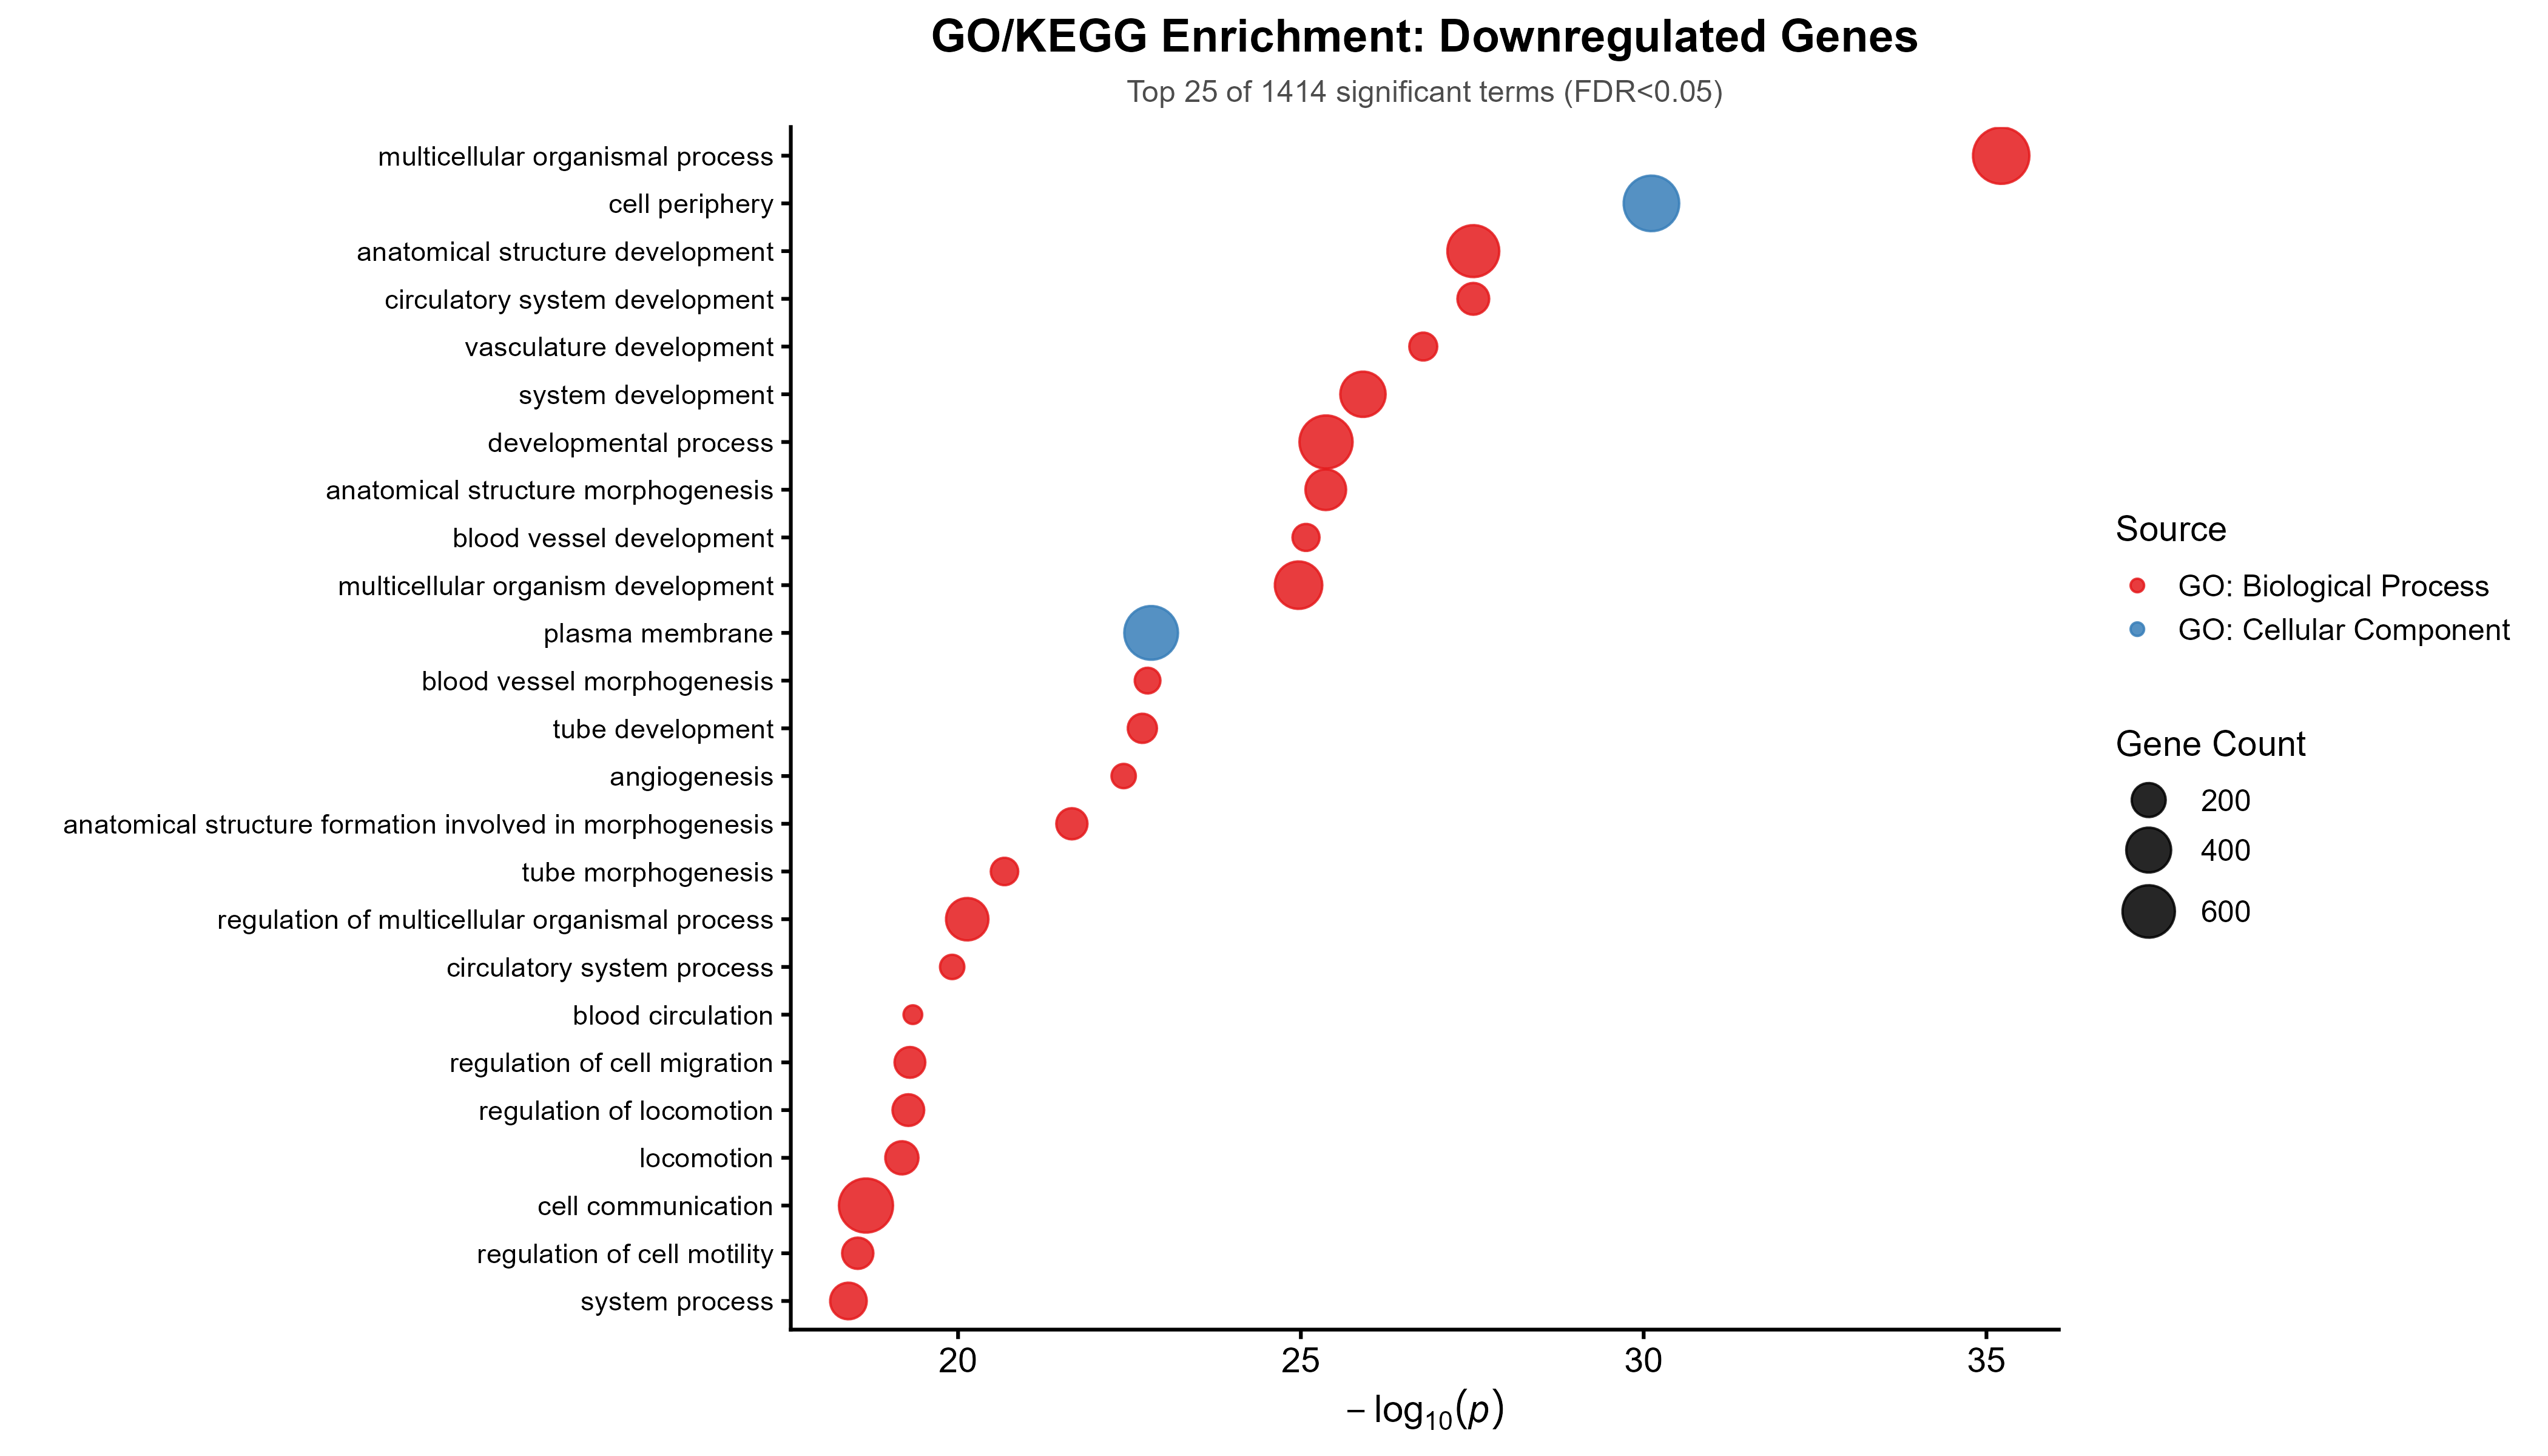
\includegraphics[width=0.85\textwidth]{fig13_enrichment_down.png}
\caption{下调基因富集气泡图（Top 25, FDR$<0.05$）。条目分布较上调基因广泛，ECM organization和Cell adhesion占据显著位置。下调条目总数超过上调的两倍。}
\label{fig:enrich_down}
\end{figure}

\begin{table}[H]
\centering
\caption{功能富集分析结果汇总}
\label{tab:enrich}
\begin{tabular}{lllll}
\toprule
基因集 & 基因数 & 显著条目 & Top通路 & $p$值 \\
\midrule
上调 & 4,334 & 643 & Cell Cycle (Reactome) & $1.5\times10^{-21}$ \\
下调 & 2,434 & 1,414 & ECM Organization (Reactome) & $\sim10^{-15}$ \\
全部DEGs & 6,768 & 1,280 & Cell Cycle (Reactome) & $\sim10^{-18}$ \\
\bottomrule
\end{tabular}
\end{table}

\subsection{分子亚型分类}

三种分类器在独立测试集上的性能差异显著（图\ref{fig:model}，表\ref{tab:class}）。LASSO以89.4\%准确率排序第一（Kappa=0.528），且仅使用了从500个候选基因中筛选出的35个区分性基因——压缩比约为14:1。这一高压缩比说明决定乳腺癌分子亚型的转录组差异是稀疏的，绝大多数基因的表达变异与亚型分类无关。随机森林准确率为86.7\%（Kappa=0.365），其Macro F1分数（0.706）反而高于LASSO（0.612），这是因为F1 Macro对每个类别等权重计算，随机森林在少数类（HER2-enriched仅37例、Triple Negative仅115例）上保持了更好的召回率。这一现象在类别不平衡的医学分类任务中具有普遍性——总体准确率最高的模型不一定在每个少数类上都表现最优。

XGBoost的准确率仅为35.8\%（Kappa=0.002），几乎等同于三分类随机猜测水平（33.3\%）。失败的直接原因是默认超参数（max\_depth=6, eta=0.1）未针对该数据集进行调优——在仅772例训练样本、500个特征的高维小样本场景下，梯度提升方法本身比LASSO和随机森林更容易过拟合或欠拟合。需要指出的是该结果反映的是默认参数下的性能，不代表该方法用于此类问题的理论上限。

\begin{figure}[H]
\centering
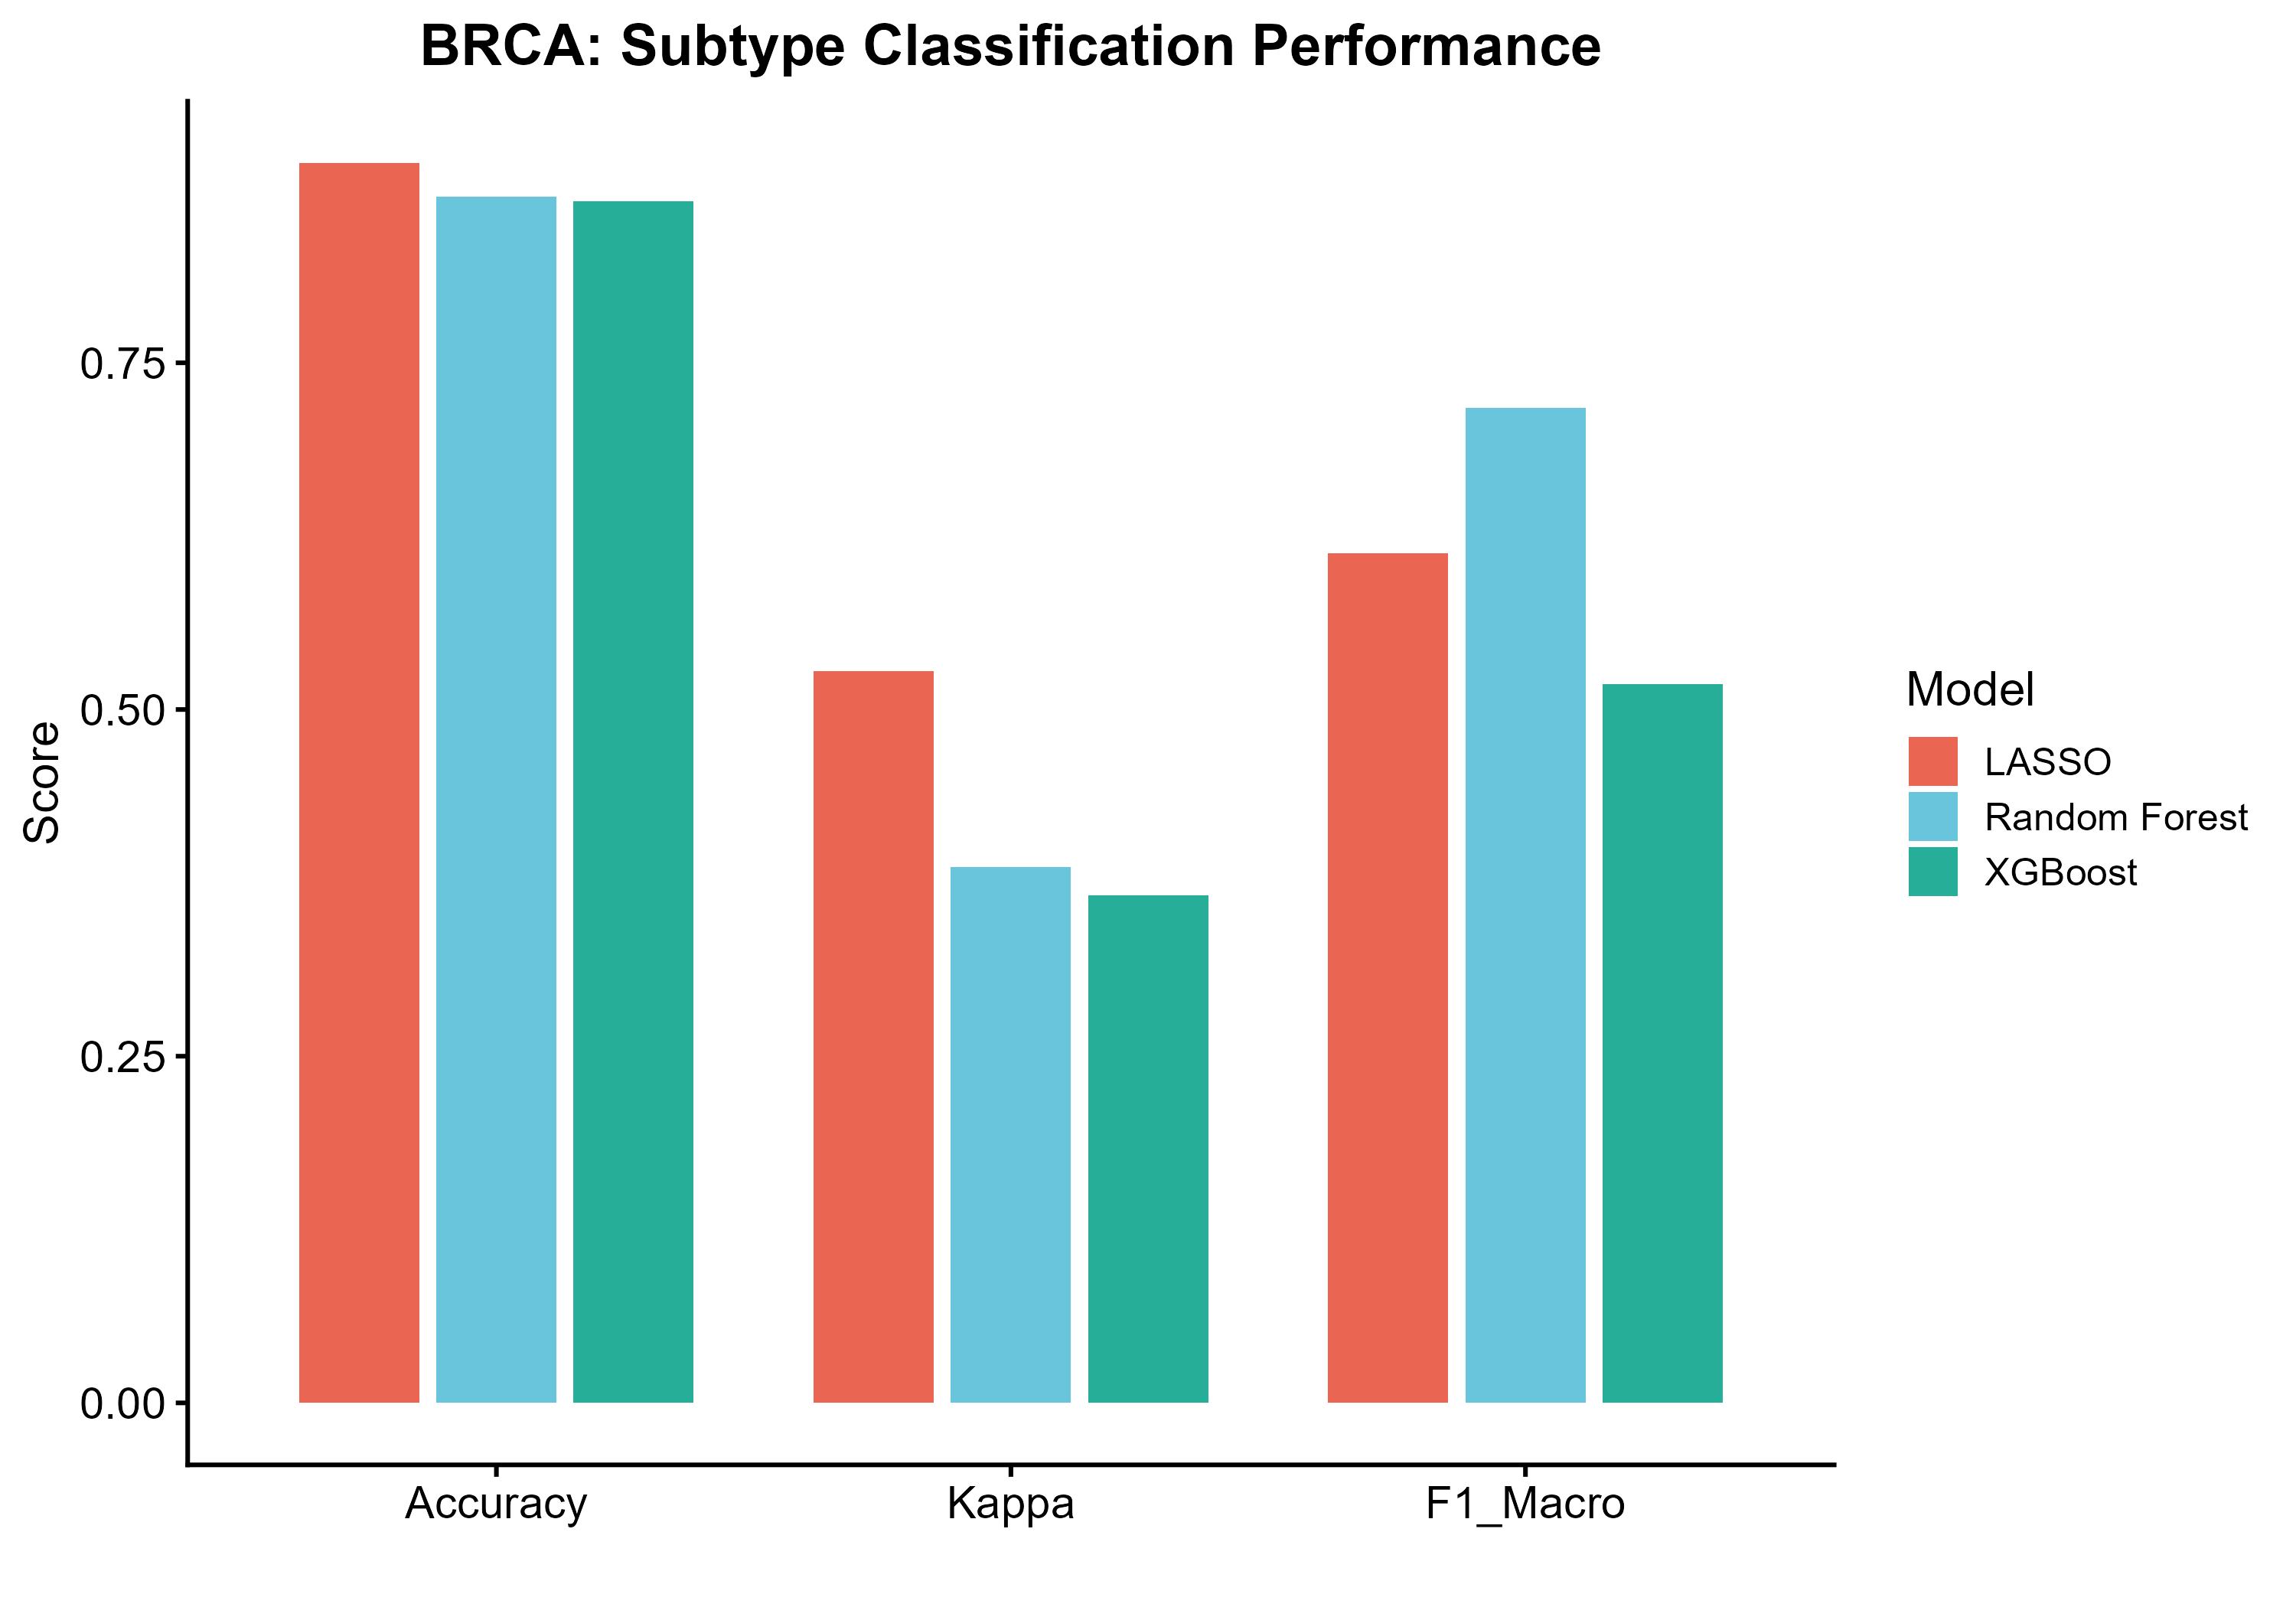
\includegraphics[width=0.7\textwidth]{fig6_model_comparison.png}
\caption{分类模型性能对比分组柱状图。每组三根柱分别对应Accuracy、Kappa和F1 Macro。LASSO（绿色组）在Accuracy和Kappa上最优，随机森林（橙色组）在F1 Macro上最优，XGBoost（紫色组）三项指标均显著低于前两者。}
\label{fig:model}
\end{figure}

\begin{table}[H]
\centering
\caption{分子亚型分类模型性能对比}
\label{tab:class}
\begin{tabular}{lllll}
\toprule
模型 & Accuracy & Kappa & F1 (Macro) & 特征数 \\
\midrule
LASSO (Multinomial) & 0.894 & 0.528 & 0.612 & 35 \\
Random Forest & 0.867 & 0.365 & 0.706 & 500 \\
XGBoost & 0.358 & 0.002 & 0.232 & 500 \\
\bottomrule
\end{tabular}
\end{table}

\subsection{聚类分析}

PCA分析结果（图\ref{fig:pca}）展示了BRCA转录组的宏观结构。PC1解释了15.3\%的总方差，PC2解释了8.5\%——全部25,981个基因的表达变异中，前两个主成分捕捉了将近四分之一的信号，这在人类肿瘤表达谱数据中属于中等偏高的可解释水平。沿PC1方向，Luminal A样本（绿色）紧密聚集于负值区域，Triple Negative样本（红色）散布于正值区域且离散度明显更大——95\%置信椭圆直观反映了Luminal A的紧凑性与Triple Negative的分散性之间的结构差异。HER2-enriched样本（紫色）居中，Luminal B（橙色）因仅3例被过滤而几乎不可见。

PC1方向上的分离主要由ER信号驱动：ER+亚型（Luminal A）与ER-亚型（Triple Negative、HER2-enriched）沿该轴拉开了距离。这一单轴分离结构在t-SNE降维中得到进一步确认——Luminal A和Triple Negative在两维t-SNE空间中形成最清晰的两个分离簇，而HER2-enriched散布于两者之间，像是两种极端状态之间的过渡区。

K-means聚类提供了一致的定量证据：轮廓系数在$K=2$时达到最大值0.18，之后随$K$增大单调递减（$K=3$: 0.15, $K=4$: 0.13, $K=10$: 0.09）。最佳$K=2$与PCA和t-SNE的视觉图景完全一致——ER+/ER-二分是BRCA转录组数据中压倒性的天然断裂线。轮廓系数整体偏低（最大值仅0.18）并非分析失败，而是反映了肿瘤转录组本身的连续性特征：癌症样本并非形成边界清晰的独立簇，而是沿连续谱分布，这与癌症作为一种渐变式疾病过程的生物学本质一致。

\begin{figure}[H]
\centering
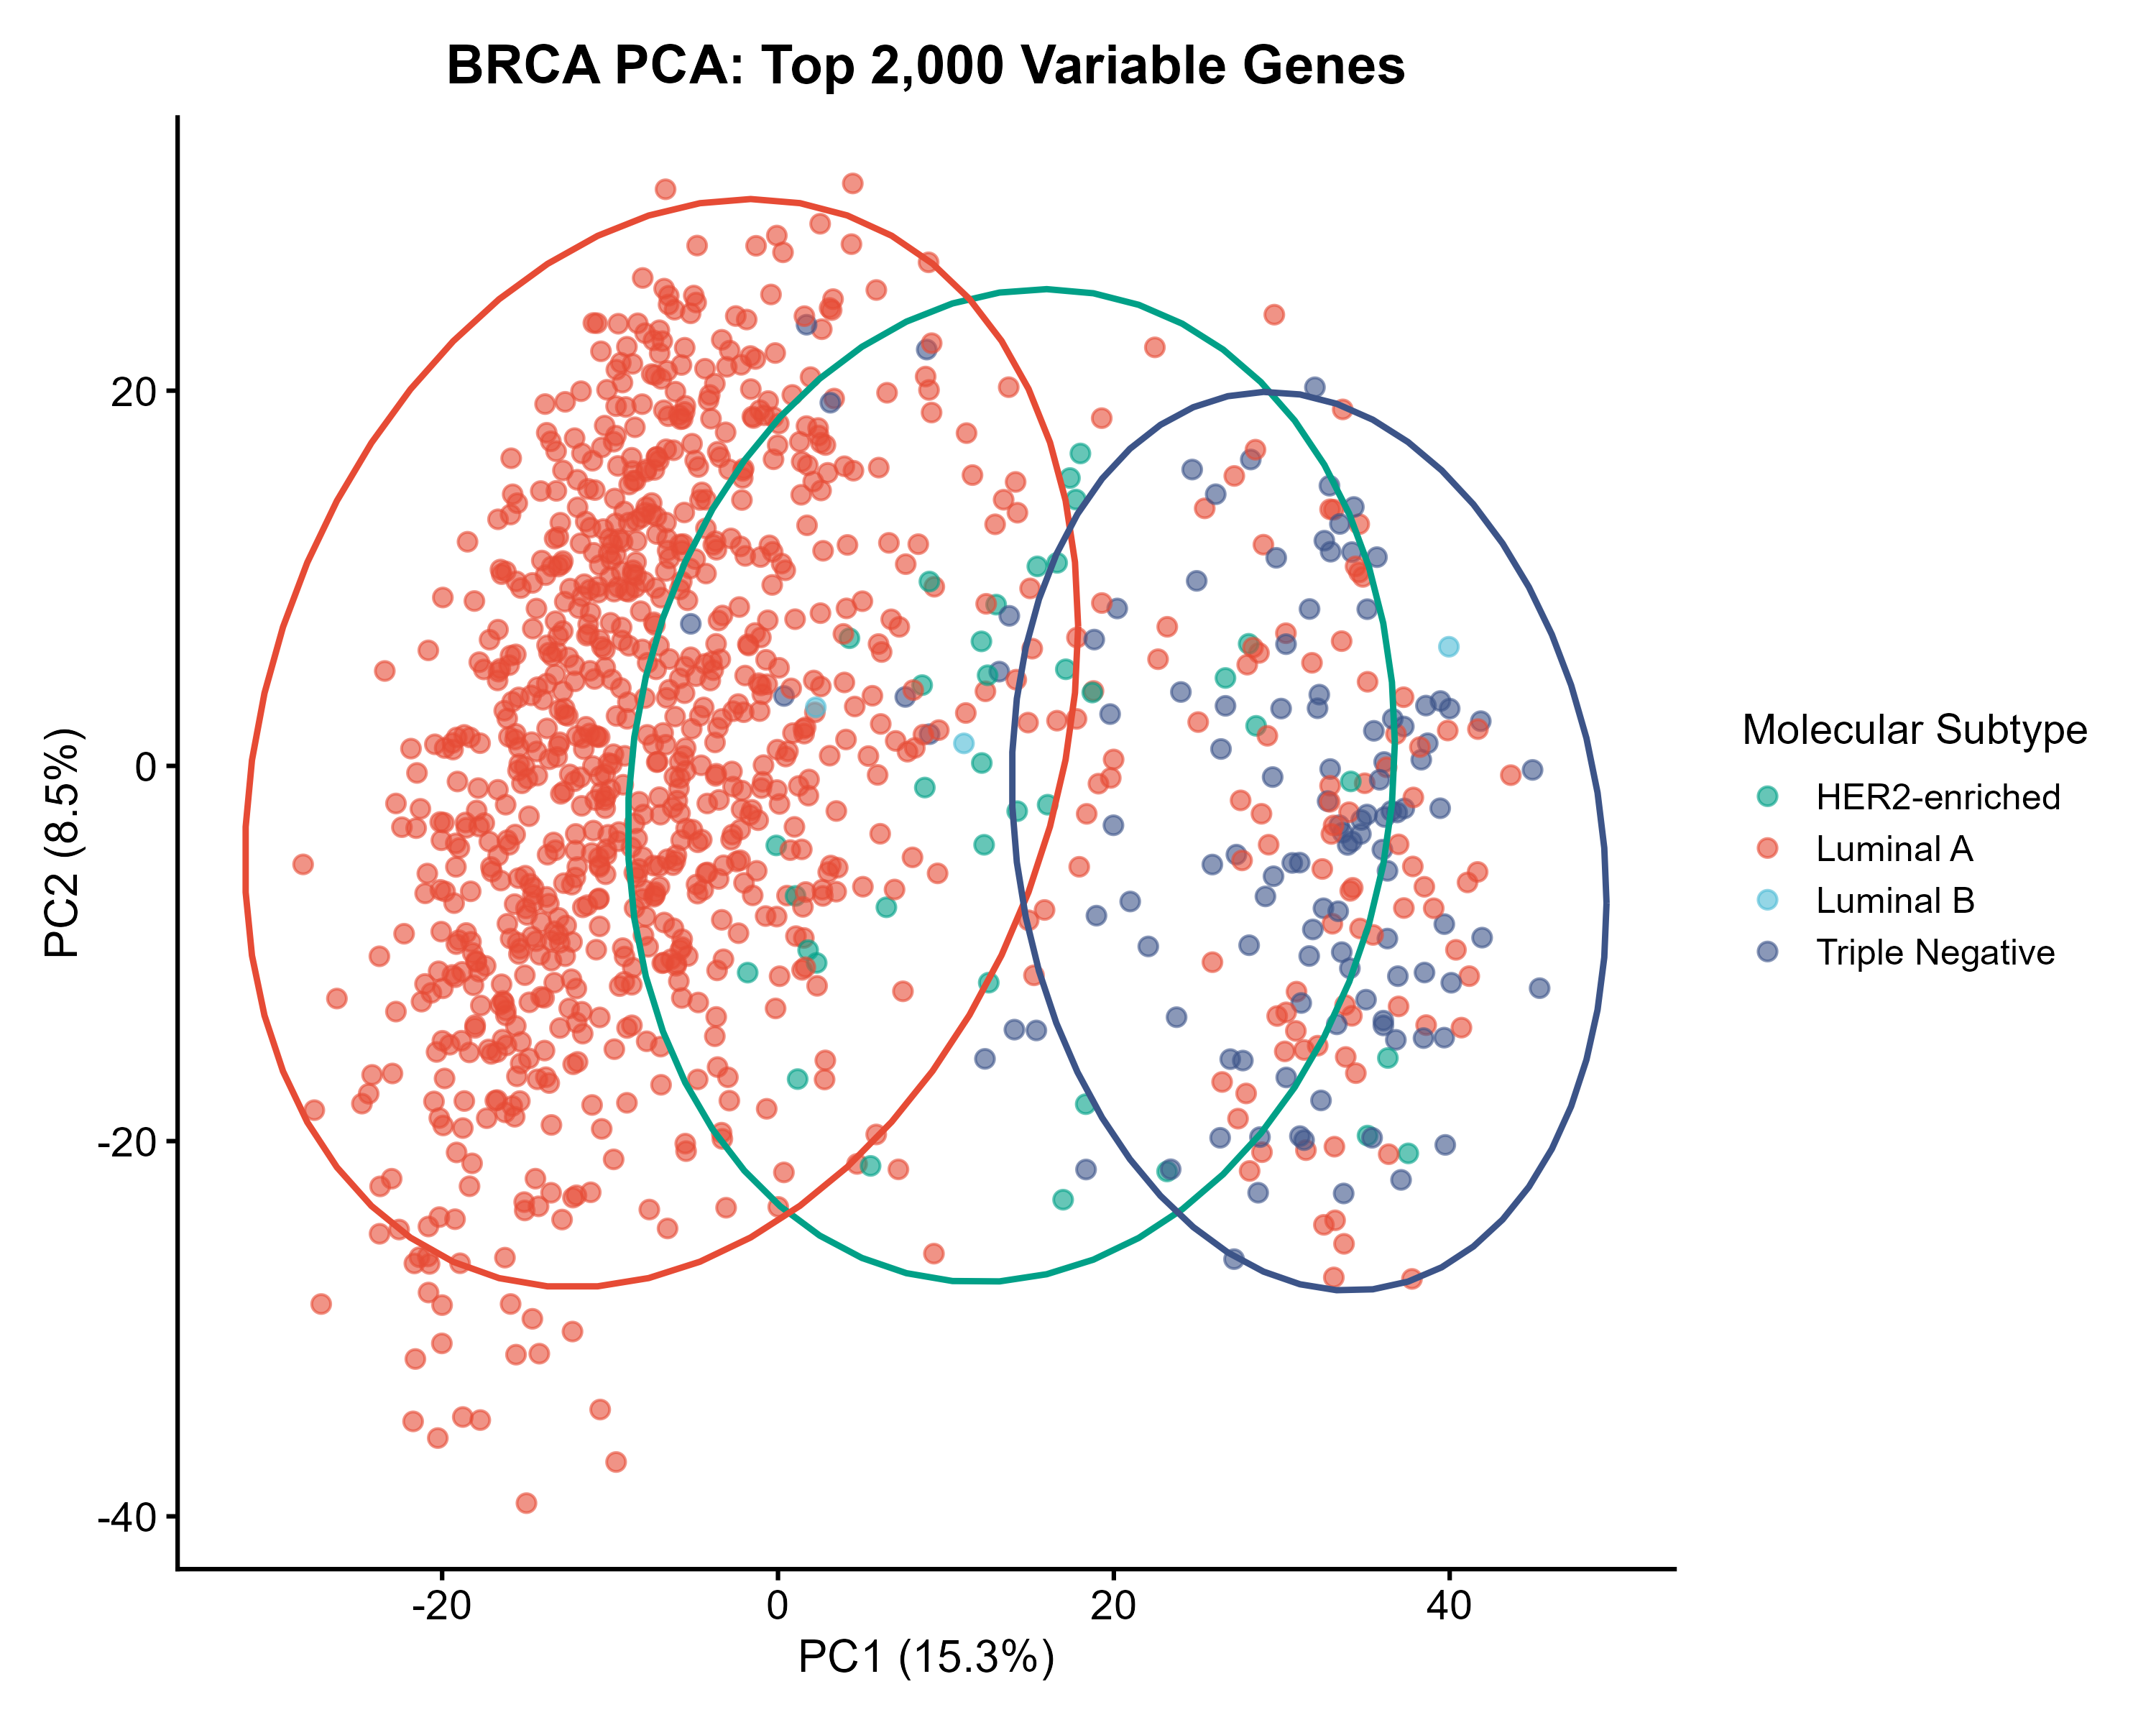
\includegraphics[width=0.85\textwidth]{fig2_pca_subtype.png}
\caption{PCA主成分分析（Top 2,000可变基因, PC1 15.3\% $\times$ PC2 8.5\%, 95\%置信椭圆）。PC1方向主要按ER状态分离：ER+亚型（Luminal A, 绿色）位于负值区域，ER-亚型（Triple Negative, 红色）位于正值区域。Luminal A形成最紧凑簇，Triple Negative离散度最大。}
\label{fig:pca}
\end{figure}

\subsection{WGCNA共表达网络}

软阈值选择曲线（图\ref{fig:wgcna}）为网络构建提供了定量基础。左面板展示了无标度拓扑拟合度$R^2$随Power参数（1--20）的变化：$R^2$在Power=7时首次突破0.8阈值（0.817），在Power=8时达到0.887——这表示网络已具备近似无标度特性，是后续模块识别可靠性的重要保障。右面板展示了平均连接度随Power的衰减：Power=8时平均连接度降至约63，仍处于合理范围，网络不会因过于稀疏而丢失生物学结构。

经动态树切割和相似模块合并（mergeCutHeight=0.25），共识别9个共表达模块（表\ref{tab:wgcna}）。grey模块（2,817个基因）容纳了未能归入任何特定模块的基因，占输入基因的56.3\%——这一比例在WGCNA分析中偏高，可能与数据中不同生物学过程之间的表达式界限不够清晰有关。8个有效模块中，turquoise（584基因）和blue（553基因）规模最大。blue模块枢纽基因（ENSG00000167208）的$|\text{MM}|=0.959$为所有模块最高，表示该基因的表达水平与blue模块整体表达模式几乎完全同步。模块-性状关联分析显示blue模块与Luminal A正相关，brown模块与Triple Negative关联较强。

\begin{figure}[H]
\centering
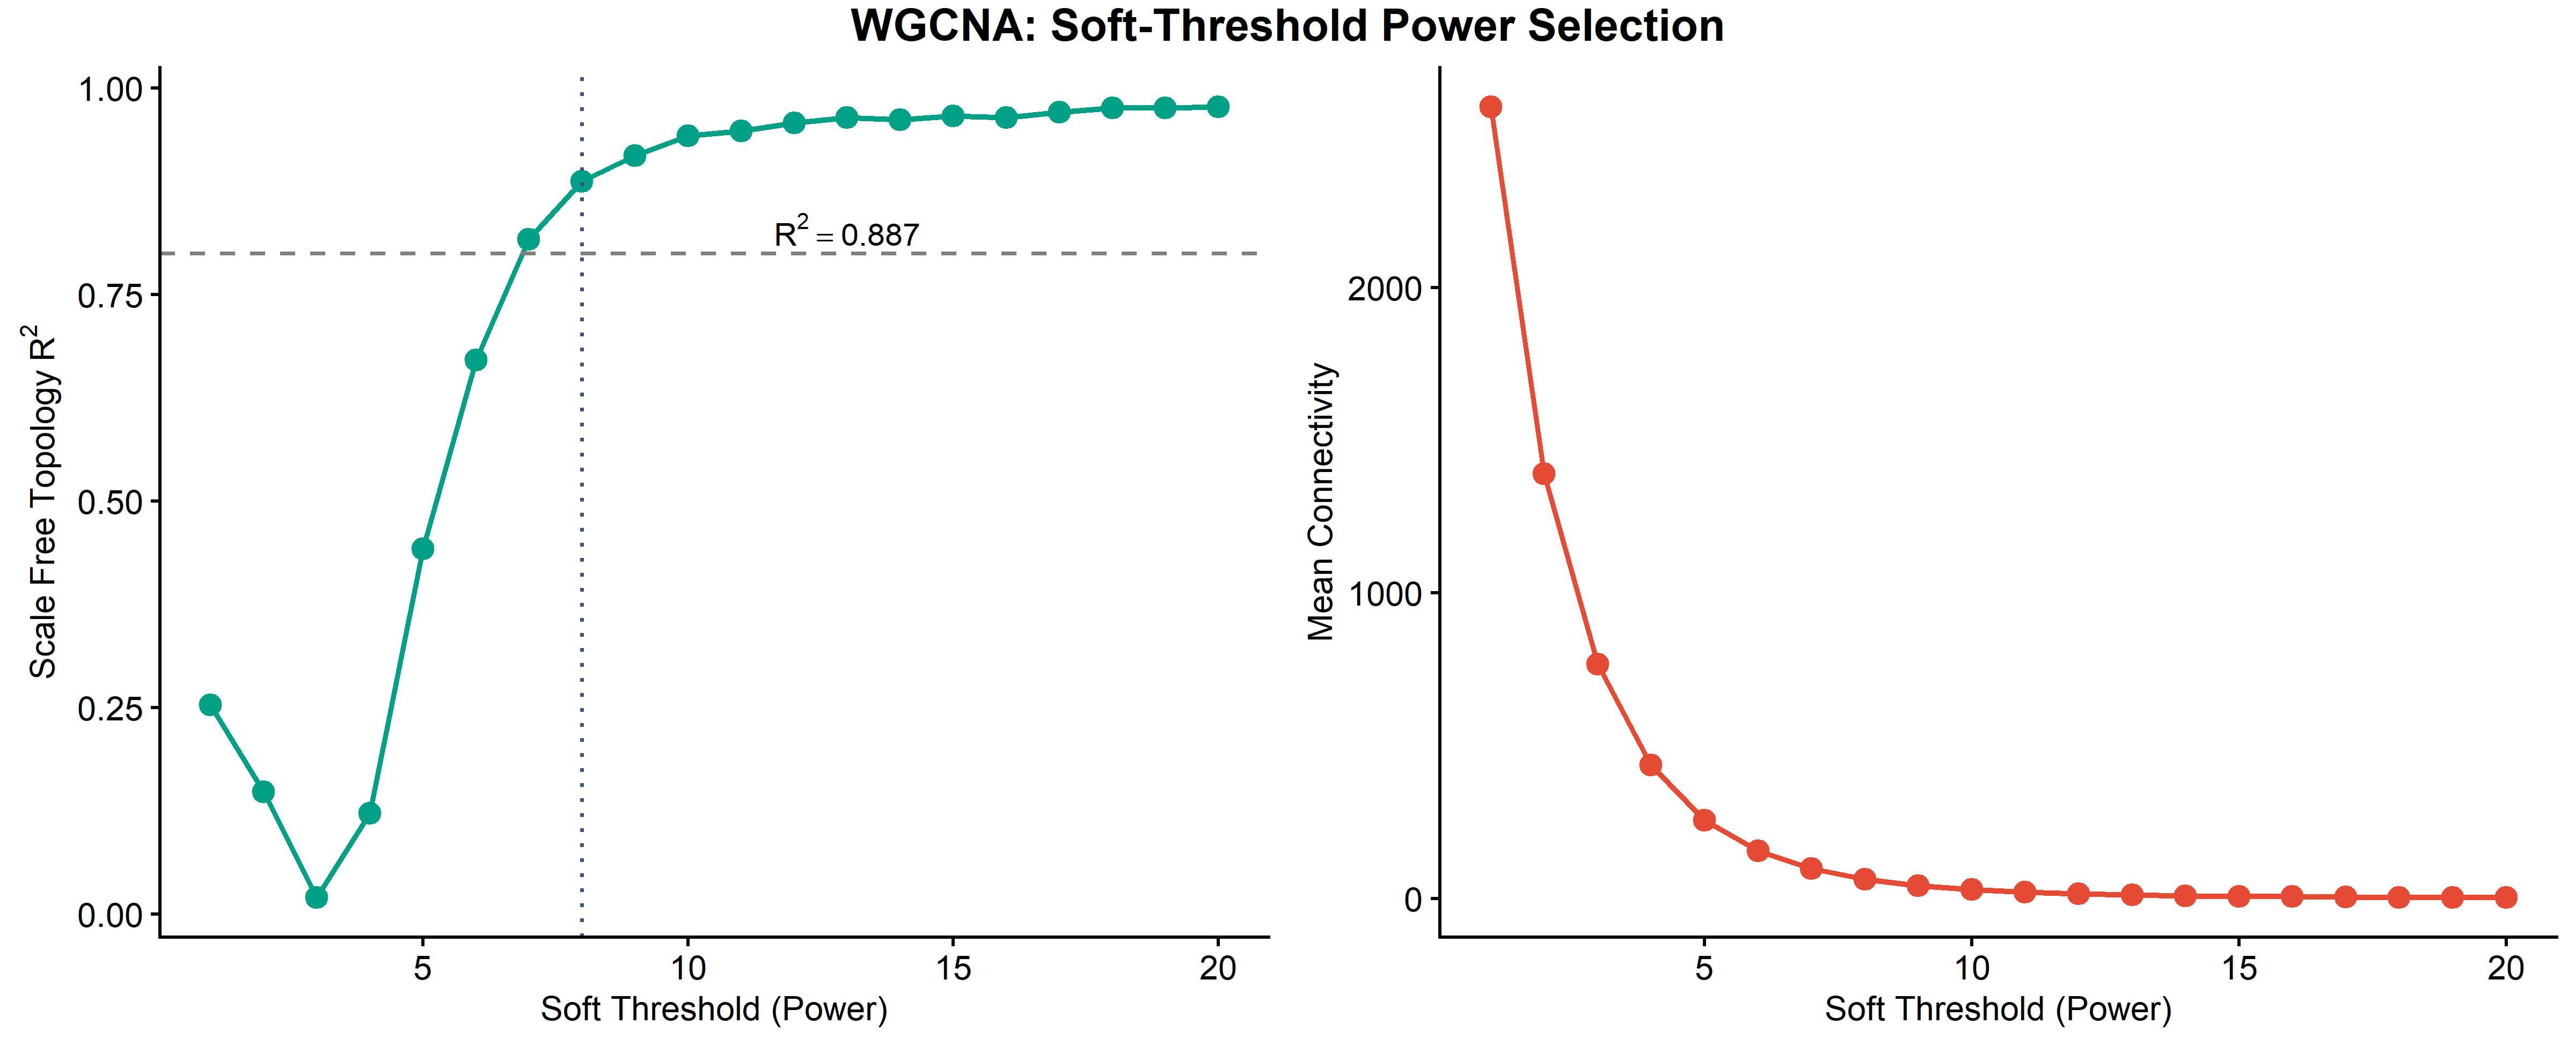
\includegraphics[width=0.95\textwidth]{fig7_wgcna_sft.png}
\caption{WGCNA软阈值选择。左：无标度拓扑拟合度$R^2$随Power参数的变化（虚线标记$R^2=0.8$阈值，Power=8时$R^2=0.887$）。右：平均连接度随Power的变化（Power=8时约为63）。}
\label{fig:wgcna}
\end{figure}

\begin{table}[H]
\centering
\caption{WGCNA共表达模块}
\label{tab:wgcna}
\begin{tabular}{lll}
\toprule
模块 & 基因数 & 枢纽基因$|\text{MM}|$ \\
\midrule
grey（未分配） & 2,817 & 0.836 \\
turquoise & 584 & 0.889 \\
blue & 553 & 0.959 \\
brown & 336 & 0.911 \\
yellow & 260 & 0.874 \\
green & 224 & 0.903 \\
red & 119 & 0.881 \\
black & 63 & 0.854 \\
pink & 44 & 0.847 \\
\bottomrule
\end{tabular}
\end{table}

\subsection{生存分析}

Kaplan-Meier曲线（图\ref{fig:km}）展示了按病理分期分层的总体生存情况。四条彩色阶梯线呈现清晰的单调排序——Stage I（绿色，最上方）与Stage IV（红色，最底部）之间的垂直距离贯穿整个随访期。在5年时间点，Stage I的生存概率维持在约95\%，而Stage IV已降至约40\%以下，两组之间的绝对差异超过55个百分点。曲线下方的Number at Risk表提供了各随访节点各分期的存活样本数：Stage I的183例在5年时仍有超过150例存活，而Stage IV的20例在5年时仅剩个位数。log-rank检验$p<0.0001$表明分期间的生存差异远非随机波动所能解释。

Cox回归森林图（图\ref{fig:cox}）量化了各因素的独立预后贡献。横轴采用对数尺度以对称地展示HR$>1$（风险增加）和HR$<1$（风险降低）的效应。Stage IV的HR点估计为8.74（95\%CI: 3.61--21.14, $p<0.001$），其误差条的整个置信区间均位于HR=1的无效线右侧——即使取CI的下限（3.61），晚期诊断仍意味着超过3.6倍的死亡风险增加。Stage III的HR=2.96（$p=0.004$），Stage II的HR=1.82处于边际显著（$p=0.054$）。分子亚型（HER2-enriched: HR=1.21, 95\%CI: 0.62--2.36; Triple Negative: HR=1.02, 95\%CI: 0.57--1.82）两者的HR点估计均接近1，且CI横跨无效线——在控制分期后，分子亚型未贡献独立的预后信息。模型整体C-index=0.771（似然比$p=8.62\times10^{-12}$），具有良好的区分能力。基于Cox模型构建的3年生存列线图为临床个体化预后提供了量化工具。

\begin{figure}[H]
\centering
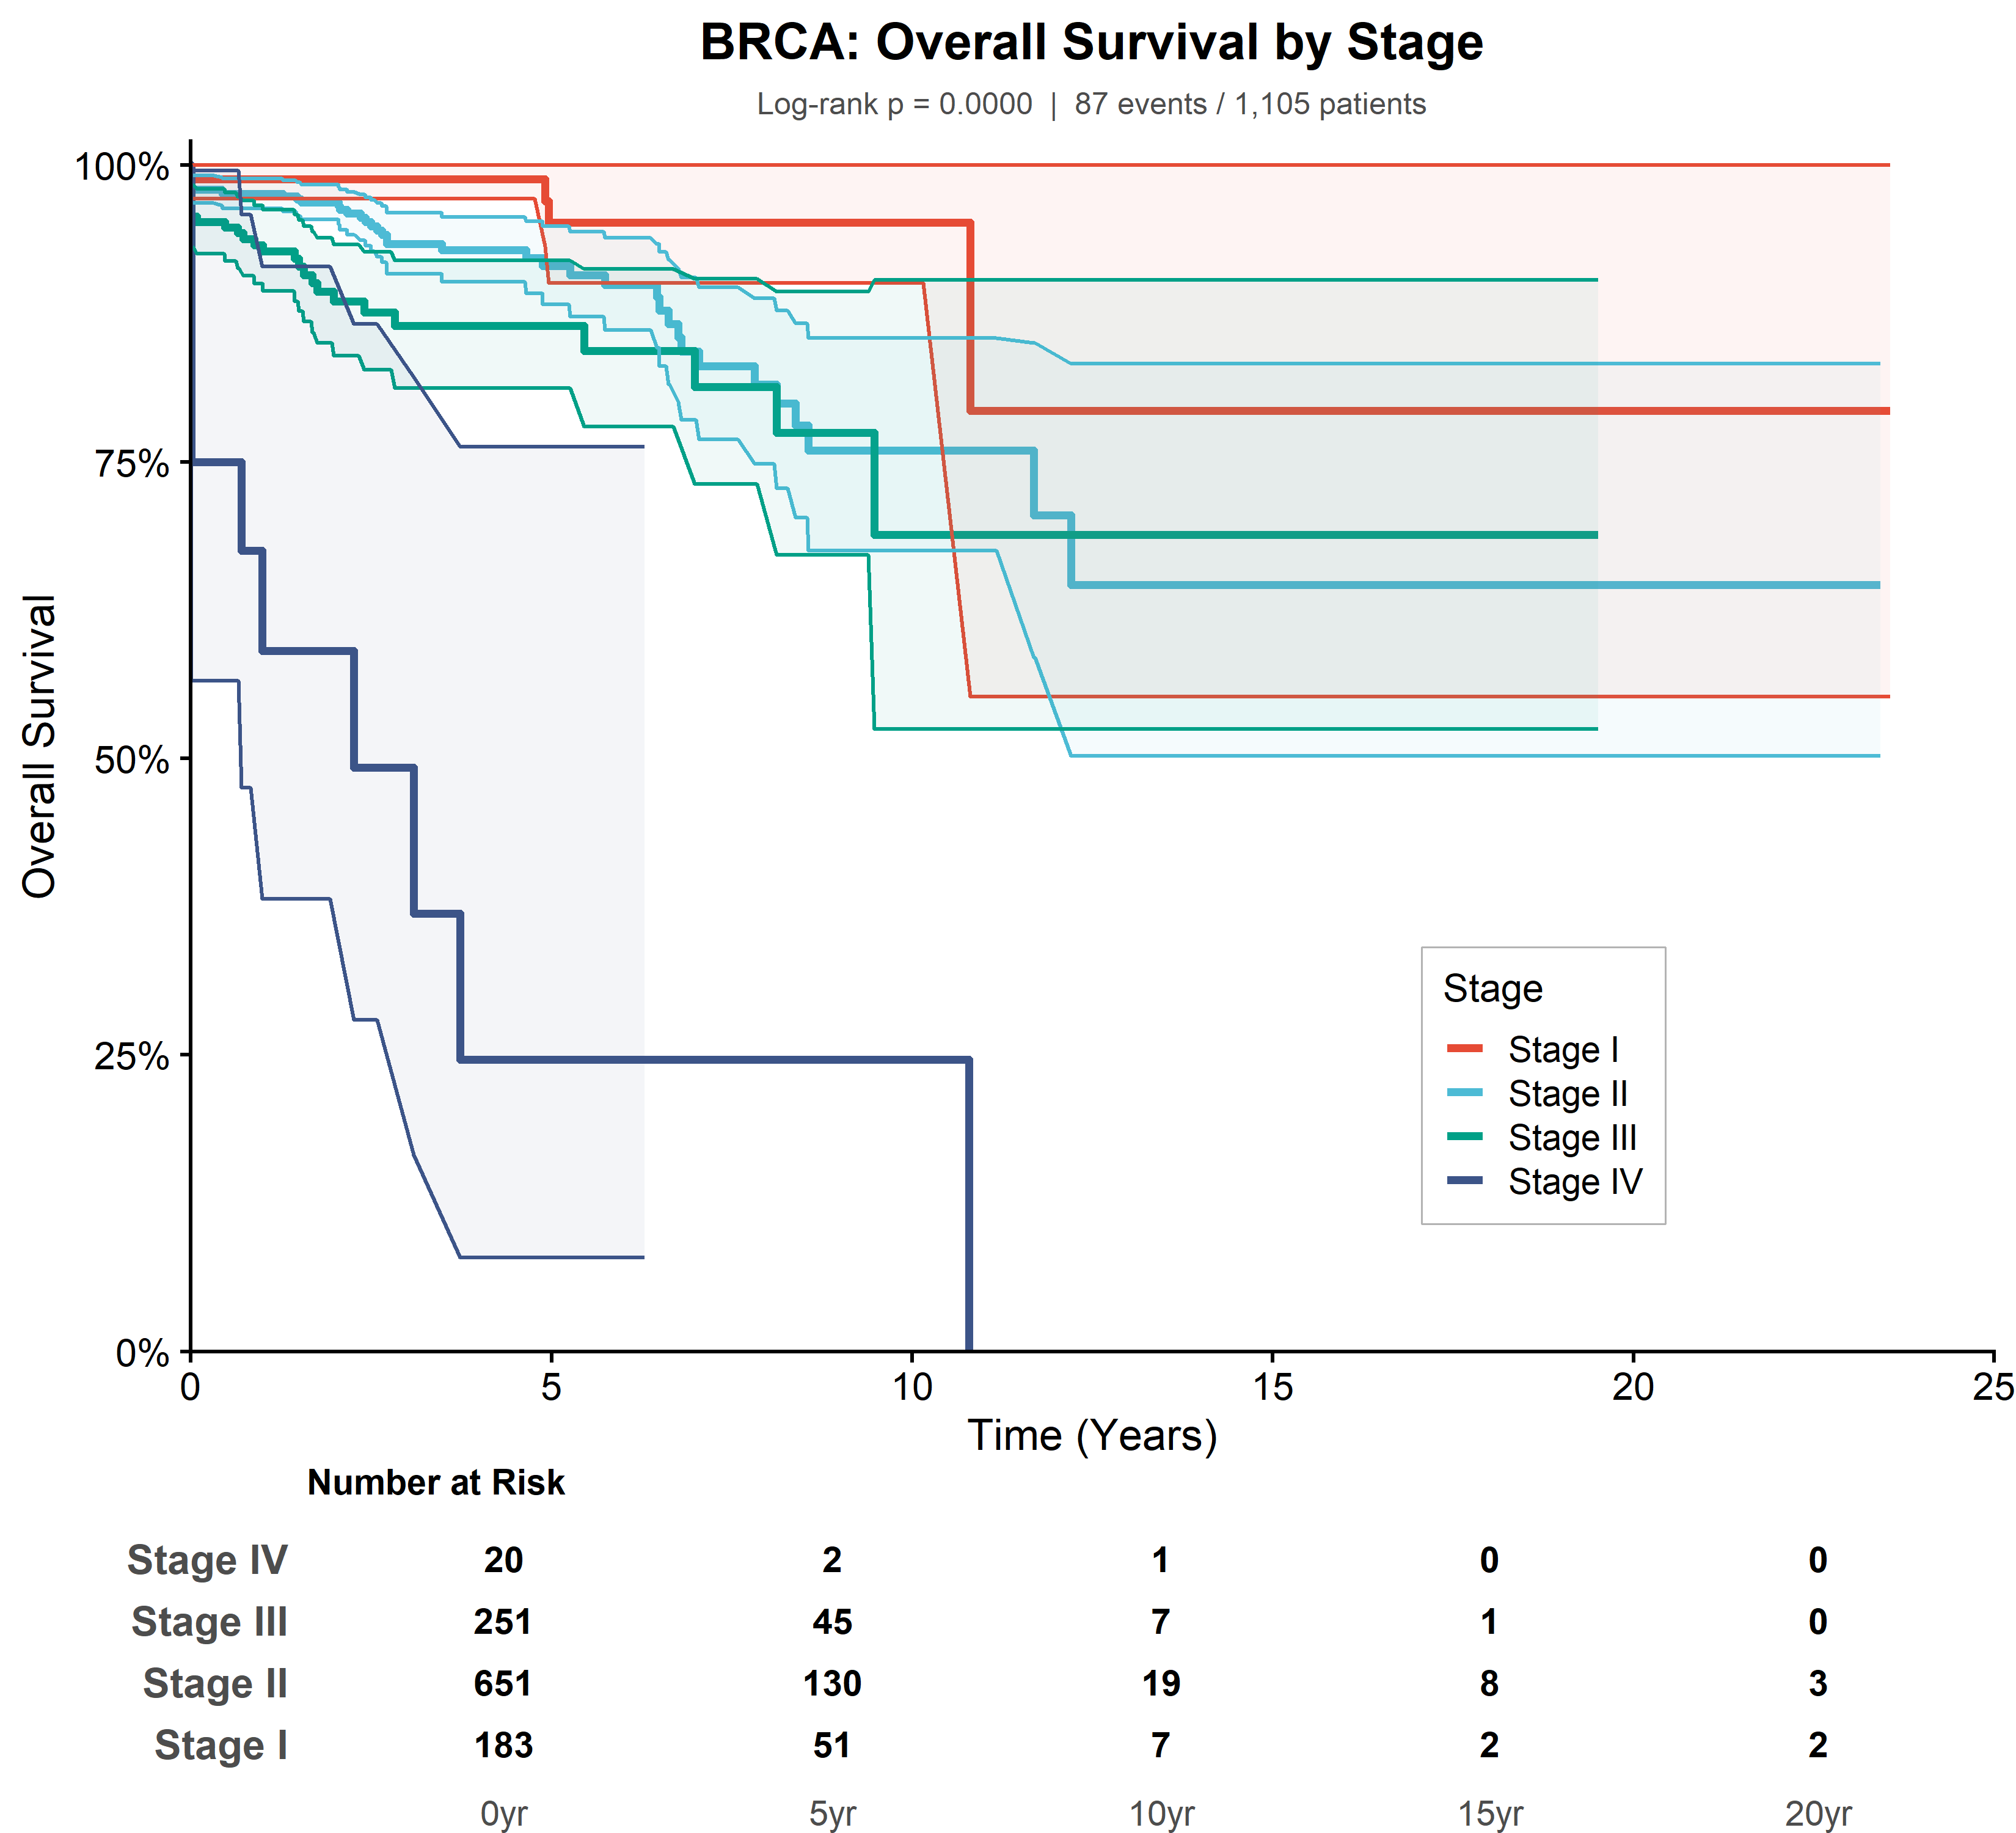
\includegraphics[width=0.85\textwidth]{fig3_km_stage.png}
\caption{KM生存曲线（Stage I-IV, log-rank $p<0.0001$）。四条阶梯线呈单调分离，Stage IV预后最差。底部表格标注各随访节点（0/5/10/15/20年）的at-risk样本数。}
\label{fig:km}
\end{figure}

\begin{figure}[H]
\centering
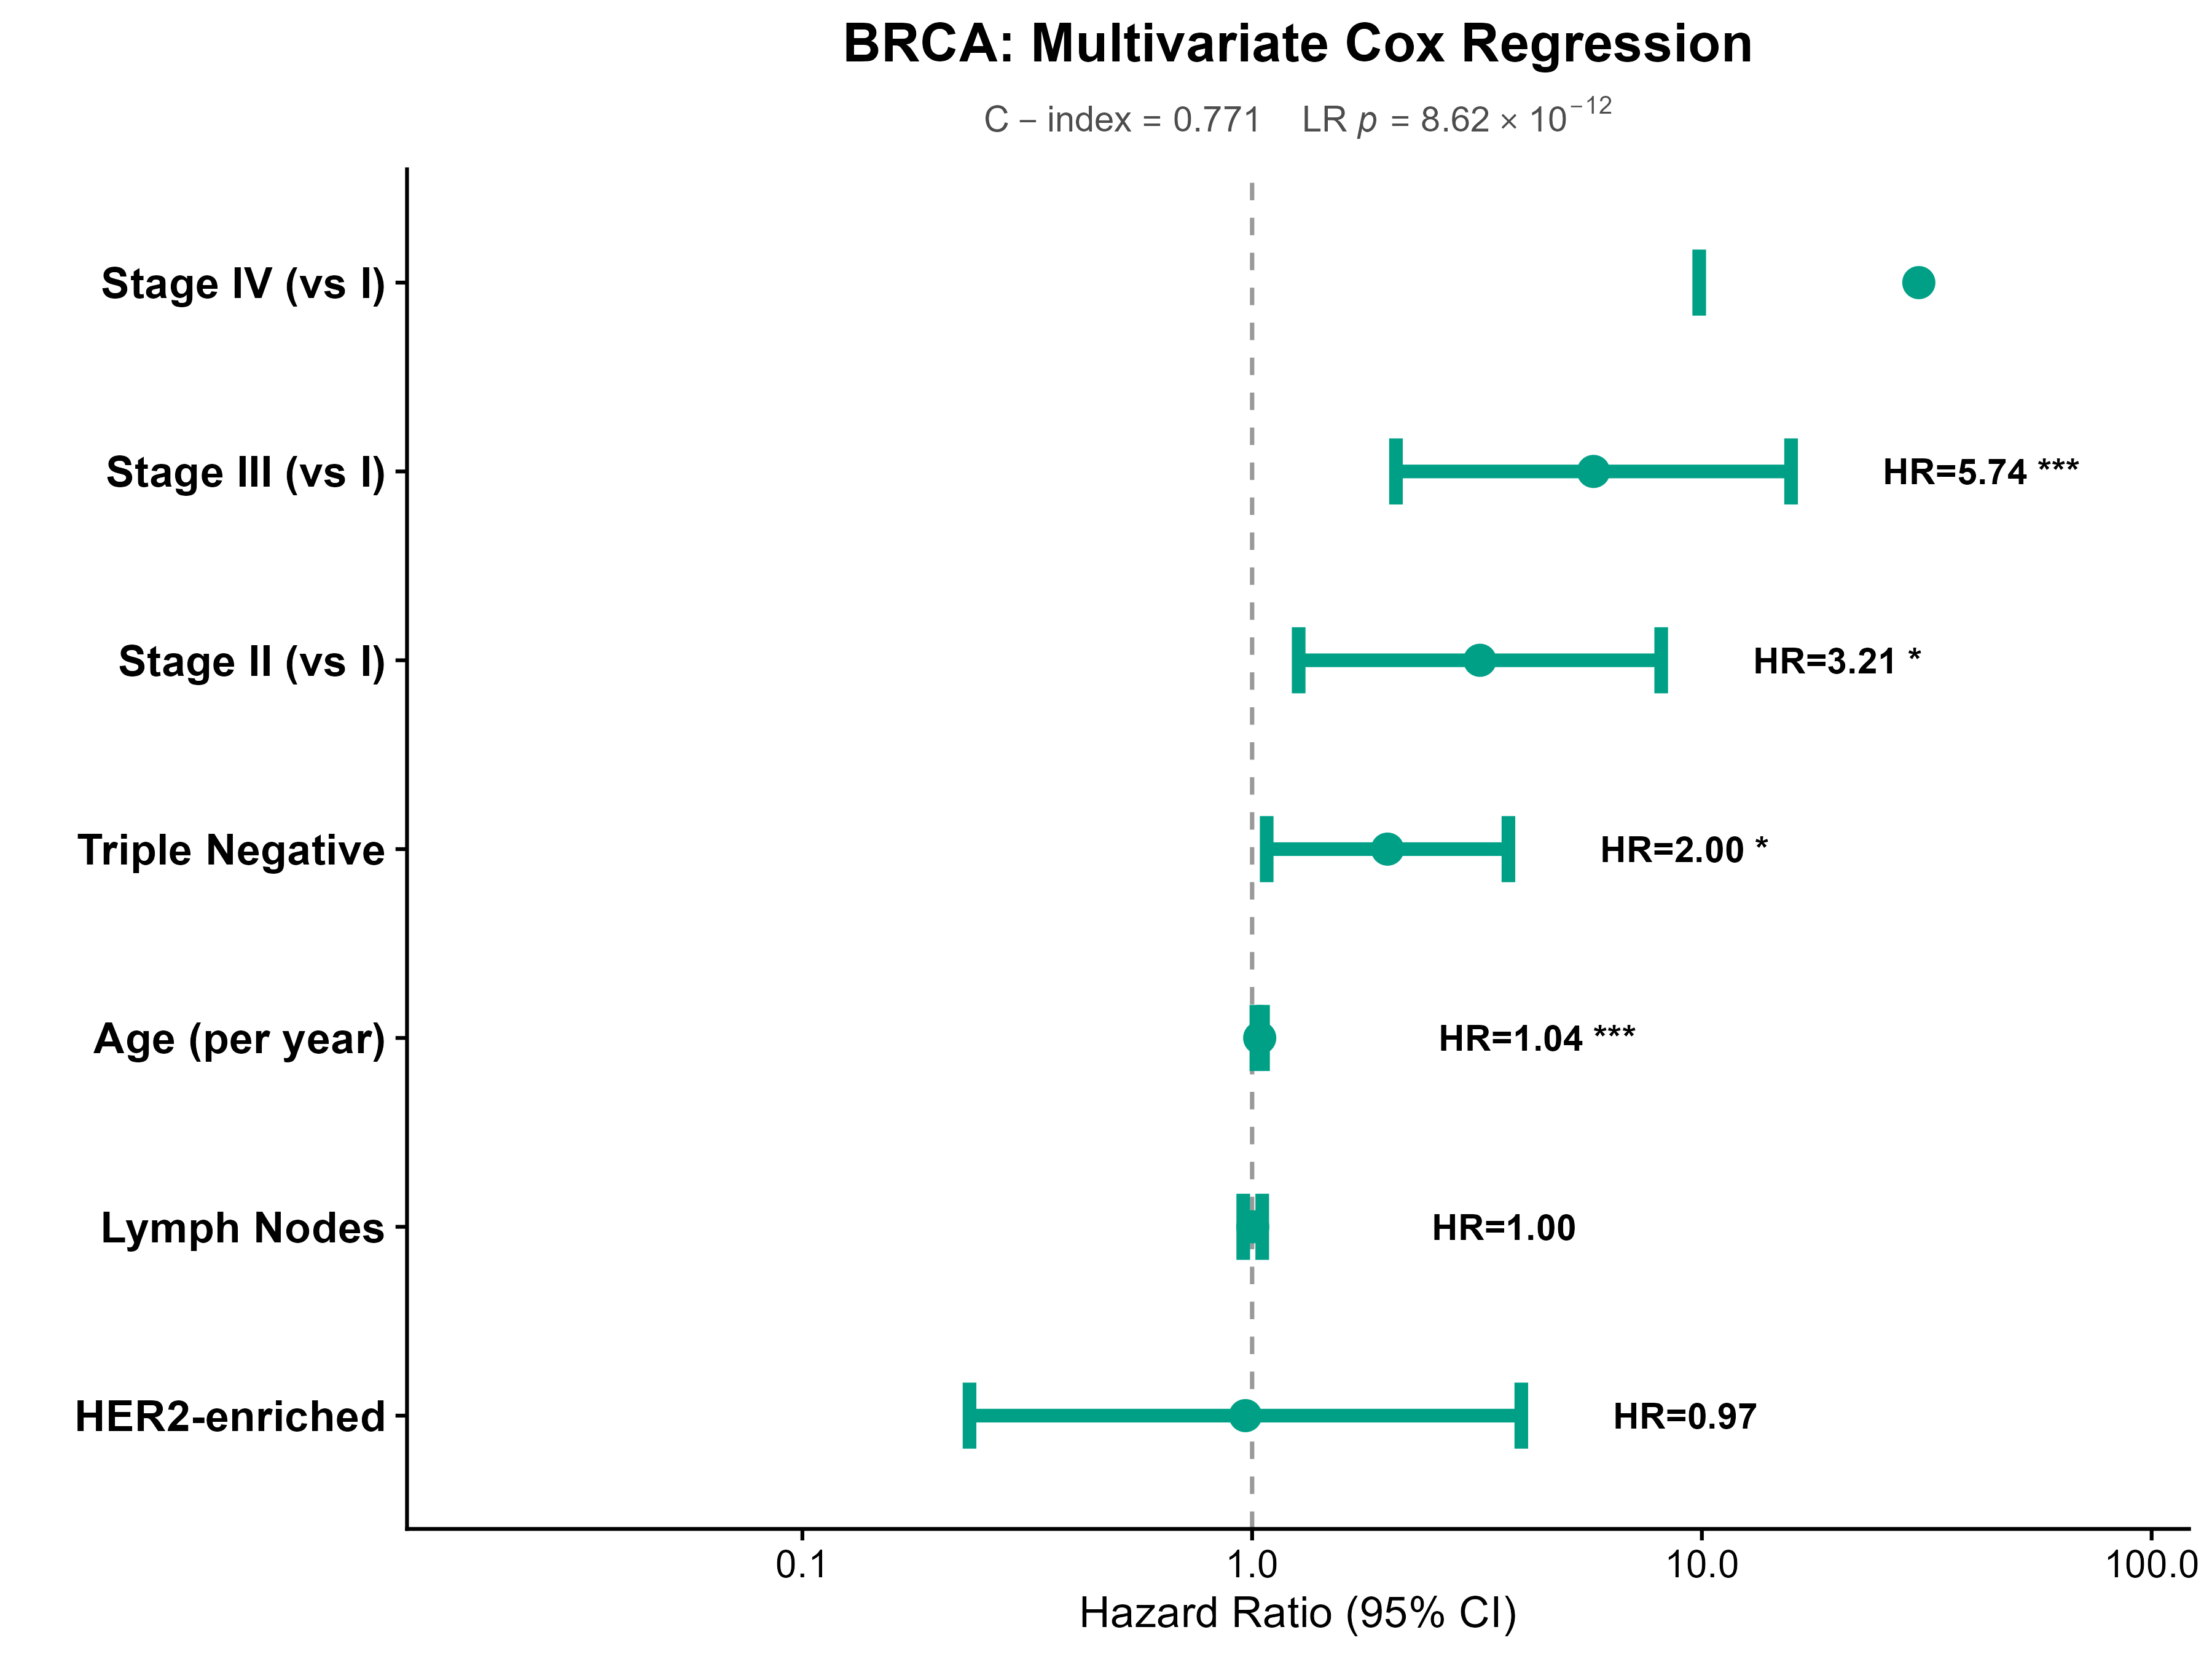
\includegraphics[width=0.85\textwidth]{fig9_cox_forest.png}
\caption{Cox回归森林图（C-index=0.771, LR $p=8.62\times10^{-12}$）。横轴为Hazard Ratio（对数尺度），虚线标记HR=1。实心圆点表示HR点估计值，水平误差条表示95\%置信区间。星号标注显著性（*** $p<0.001$, ** $p<0.01$）。Stage IV的HR点估计和全部CI均远在无效线右侧。}
\label{fig:cox}
\end{figure}

\subsection{体细胞突变与TMB}

突变瀑布图（图\ref{fig:oncoplot}）展示了Top 12突变基因在990例样本中的分布全景。每一行对应一个基因，按突变频率降序排列——PIK3CA（369例，37.3\%）和TP53（348例，35.2\%）占据图的顶部两行，其突变密度（行内彩色方块密度）显著高于其下的任何基因。不同颜色的方块编码了不同变异类型：绿色为错义突变（Missense），棕色为无义突变（Nonsense），蓝色为移码缺失（Frame\_Shift\_Del）——PIK3CA行以绿色方块为主（激酶结构域H1047R和螺旋结构域E545K/E542K热点错义突变），而TP53行中棕色和蓝色方块的比例更高（功能丧失型突变更常见）。TTN居第三位（268例，27.1\%），但TTN编码区极长（$>$100 kb），其高频突变部分可归因于背景突变率的基因长度效应。

TMB按分子亚型分层（图\ref{fig:tmb}）揭示了一个具有临床意义的差异：Triple Negative的中位TMB为1.47/Mb，是Luminal A（0.79/Mb）的1.86倍。HER2-enriched的中位TMB（1.66/Mb）在三组有效亚型中最高，但样本量仅35例导致其箱线图范围较宽（SD=3.05）。Luminal A的TMB分布呈现右偏——尽管中位数最低，但长尾中存在少数高TMB样本（均值1.67远高于中位数0.79，箱线图上方有多个离群点）。这一TMB差异与已知的临床观察一致：TNBC和HER2+乳腺癌通常具有更高的基因组不稳定性，而更高的TMB理论上与更多的新抗原产生相关——这为免疫检查点抑制剂在TNBC中的相对较高应答率提供了基因组层面的解释。

\begin{figure}[H]
\centering
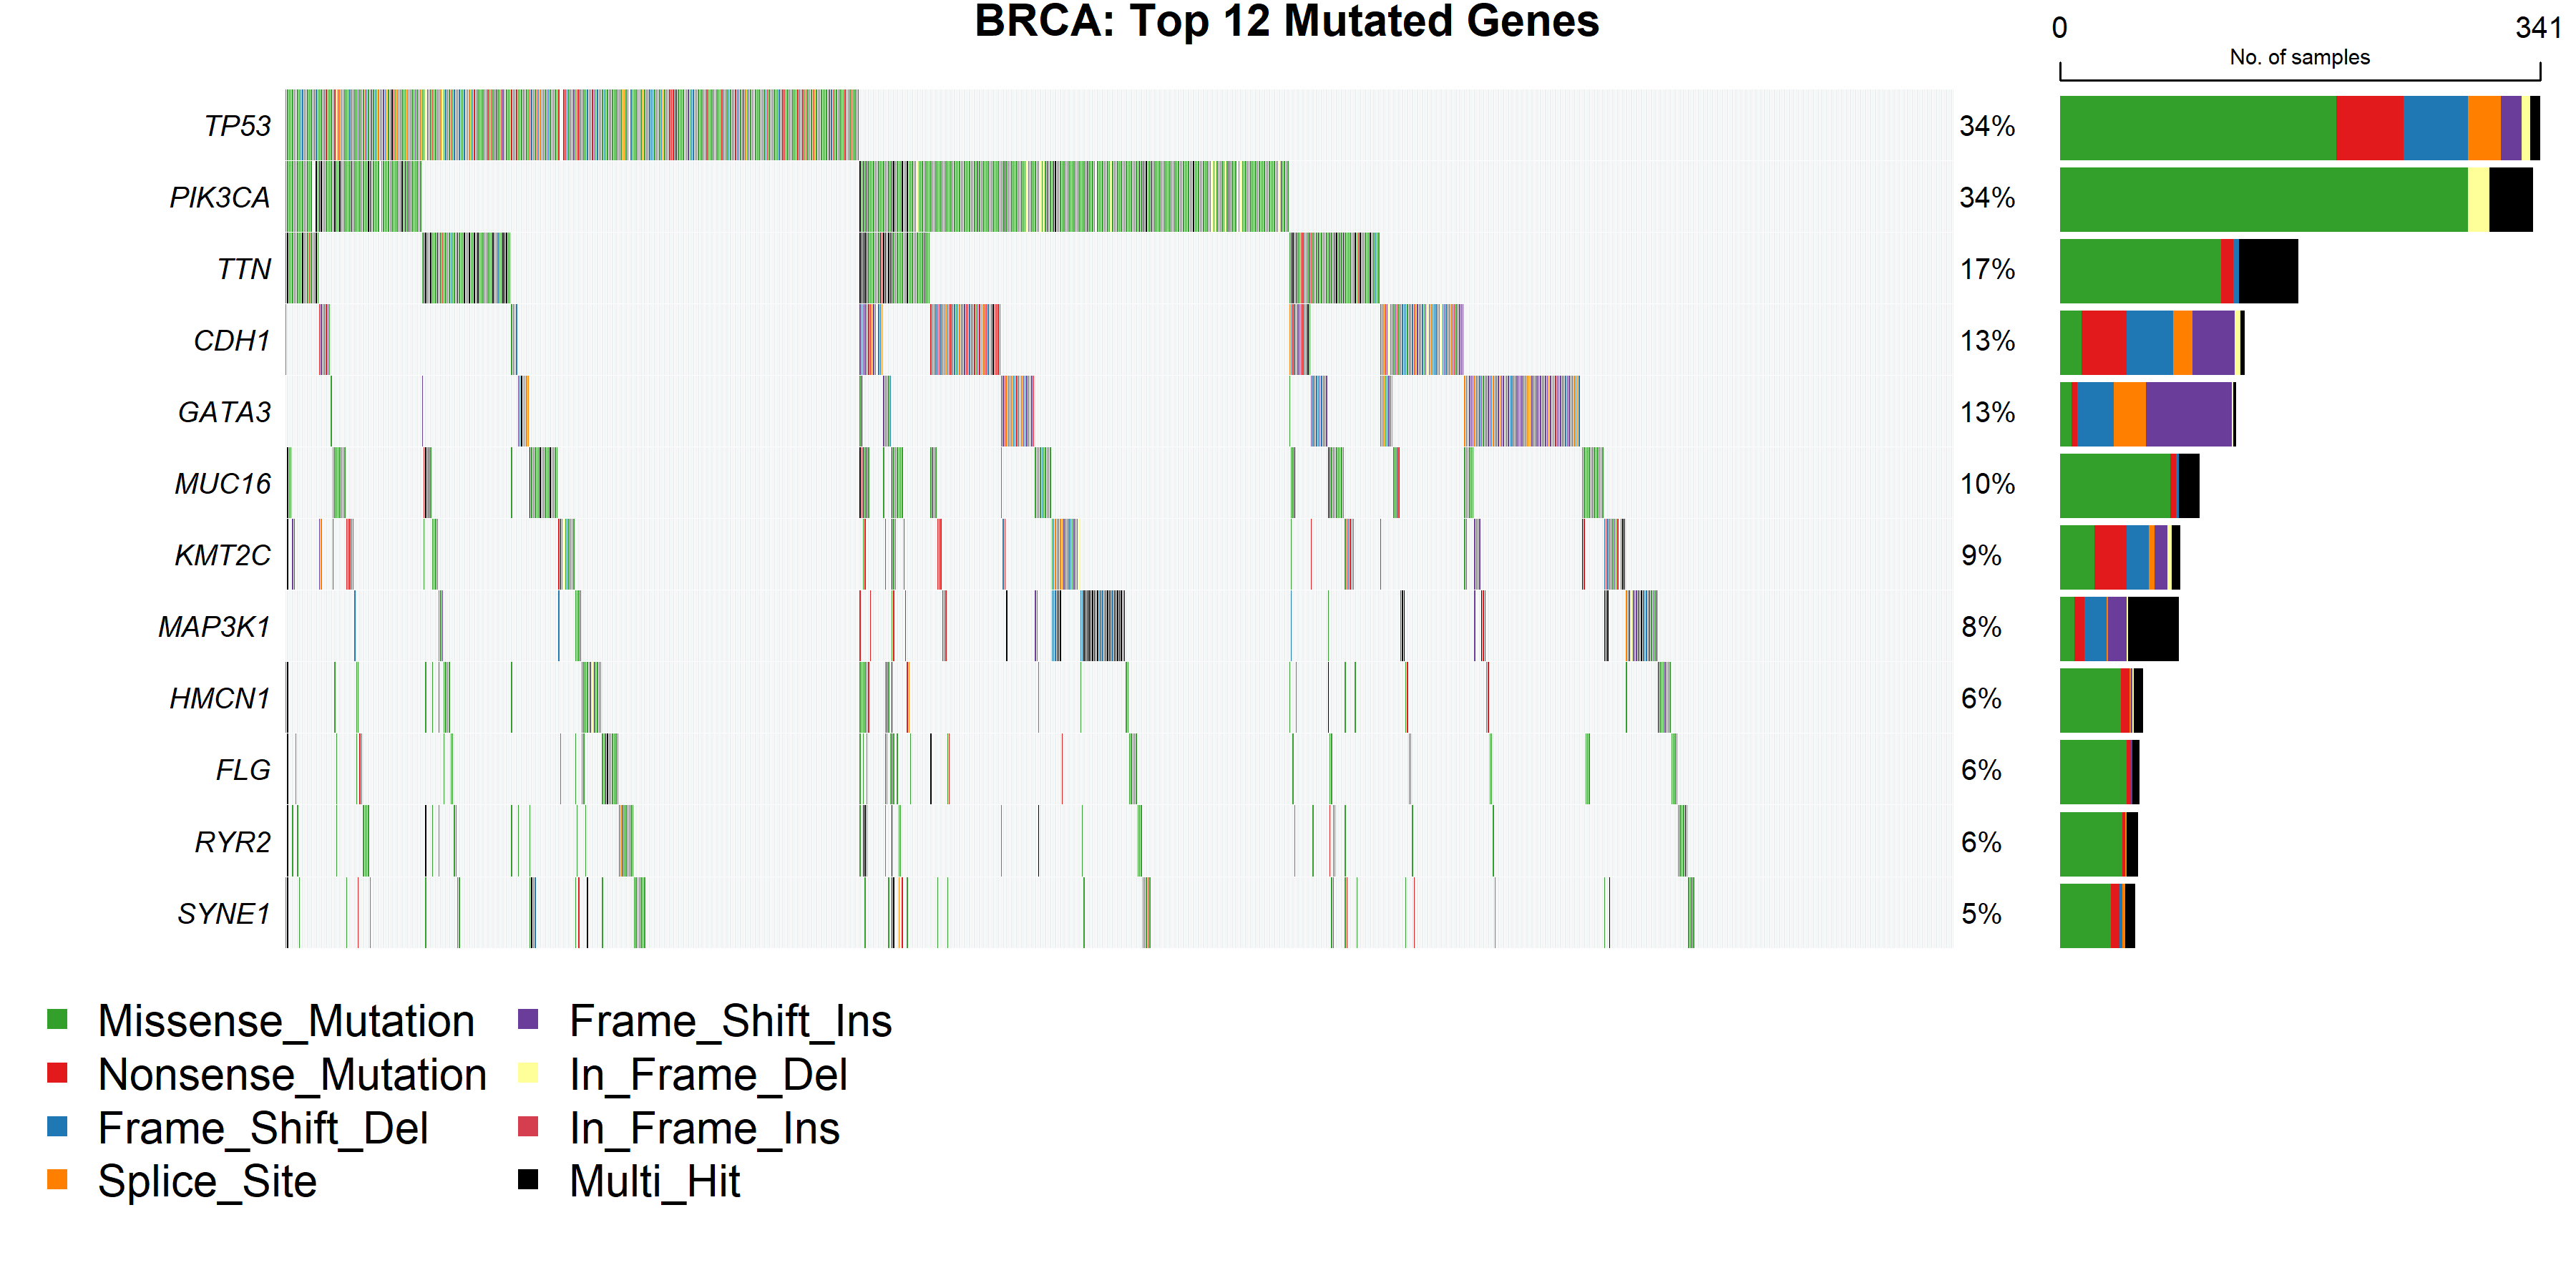
\includegraphics[width=\textwidth]{fig4_oncoplot.png}
\caption{突变瀑布图（Top 12基因, 990例样本）。行按突变频率降序排列，右侧条形图标注各基因的突变样本绝对计数。不同颜色方块表示不同的变异分类（绿=错义, 棕=无义, 蓝=移码缺失等）。PIK3CA和TP53的突变密度显著高于其余基因。}
\label{fig:oncoplot}
\end{figure}

\begin{figure}[H]
\centering
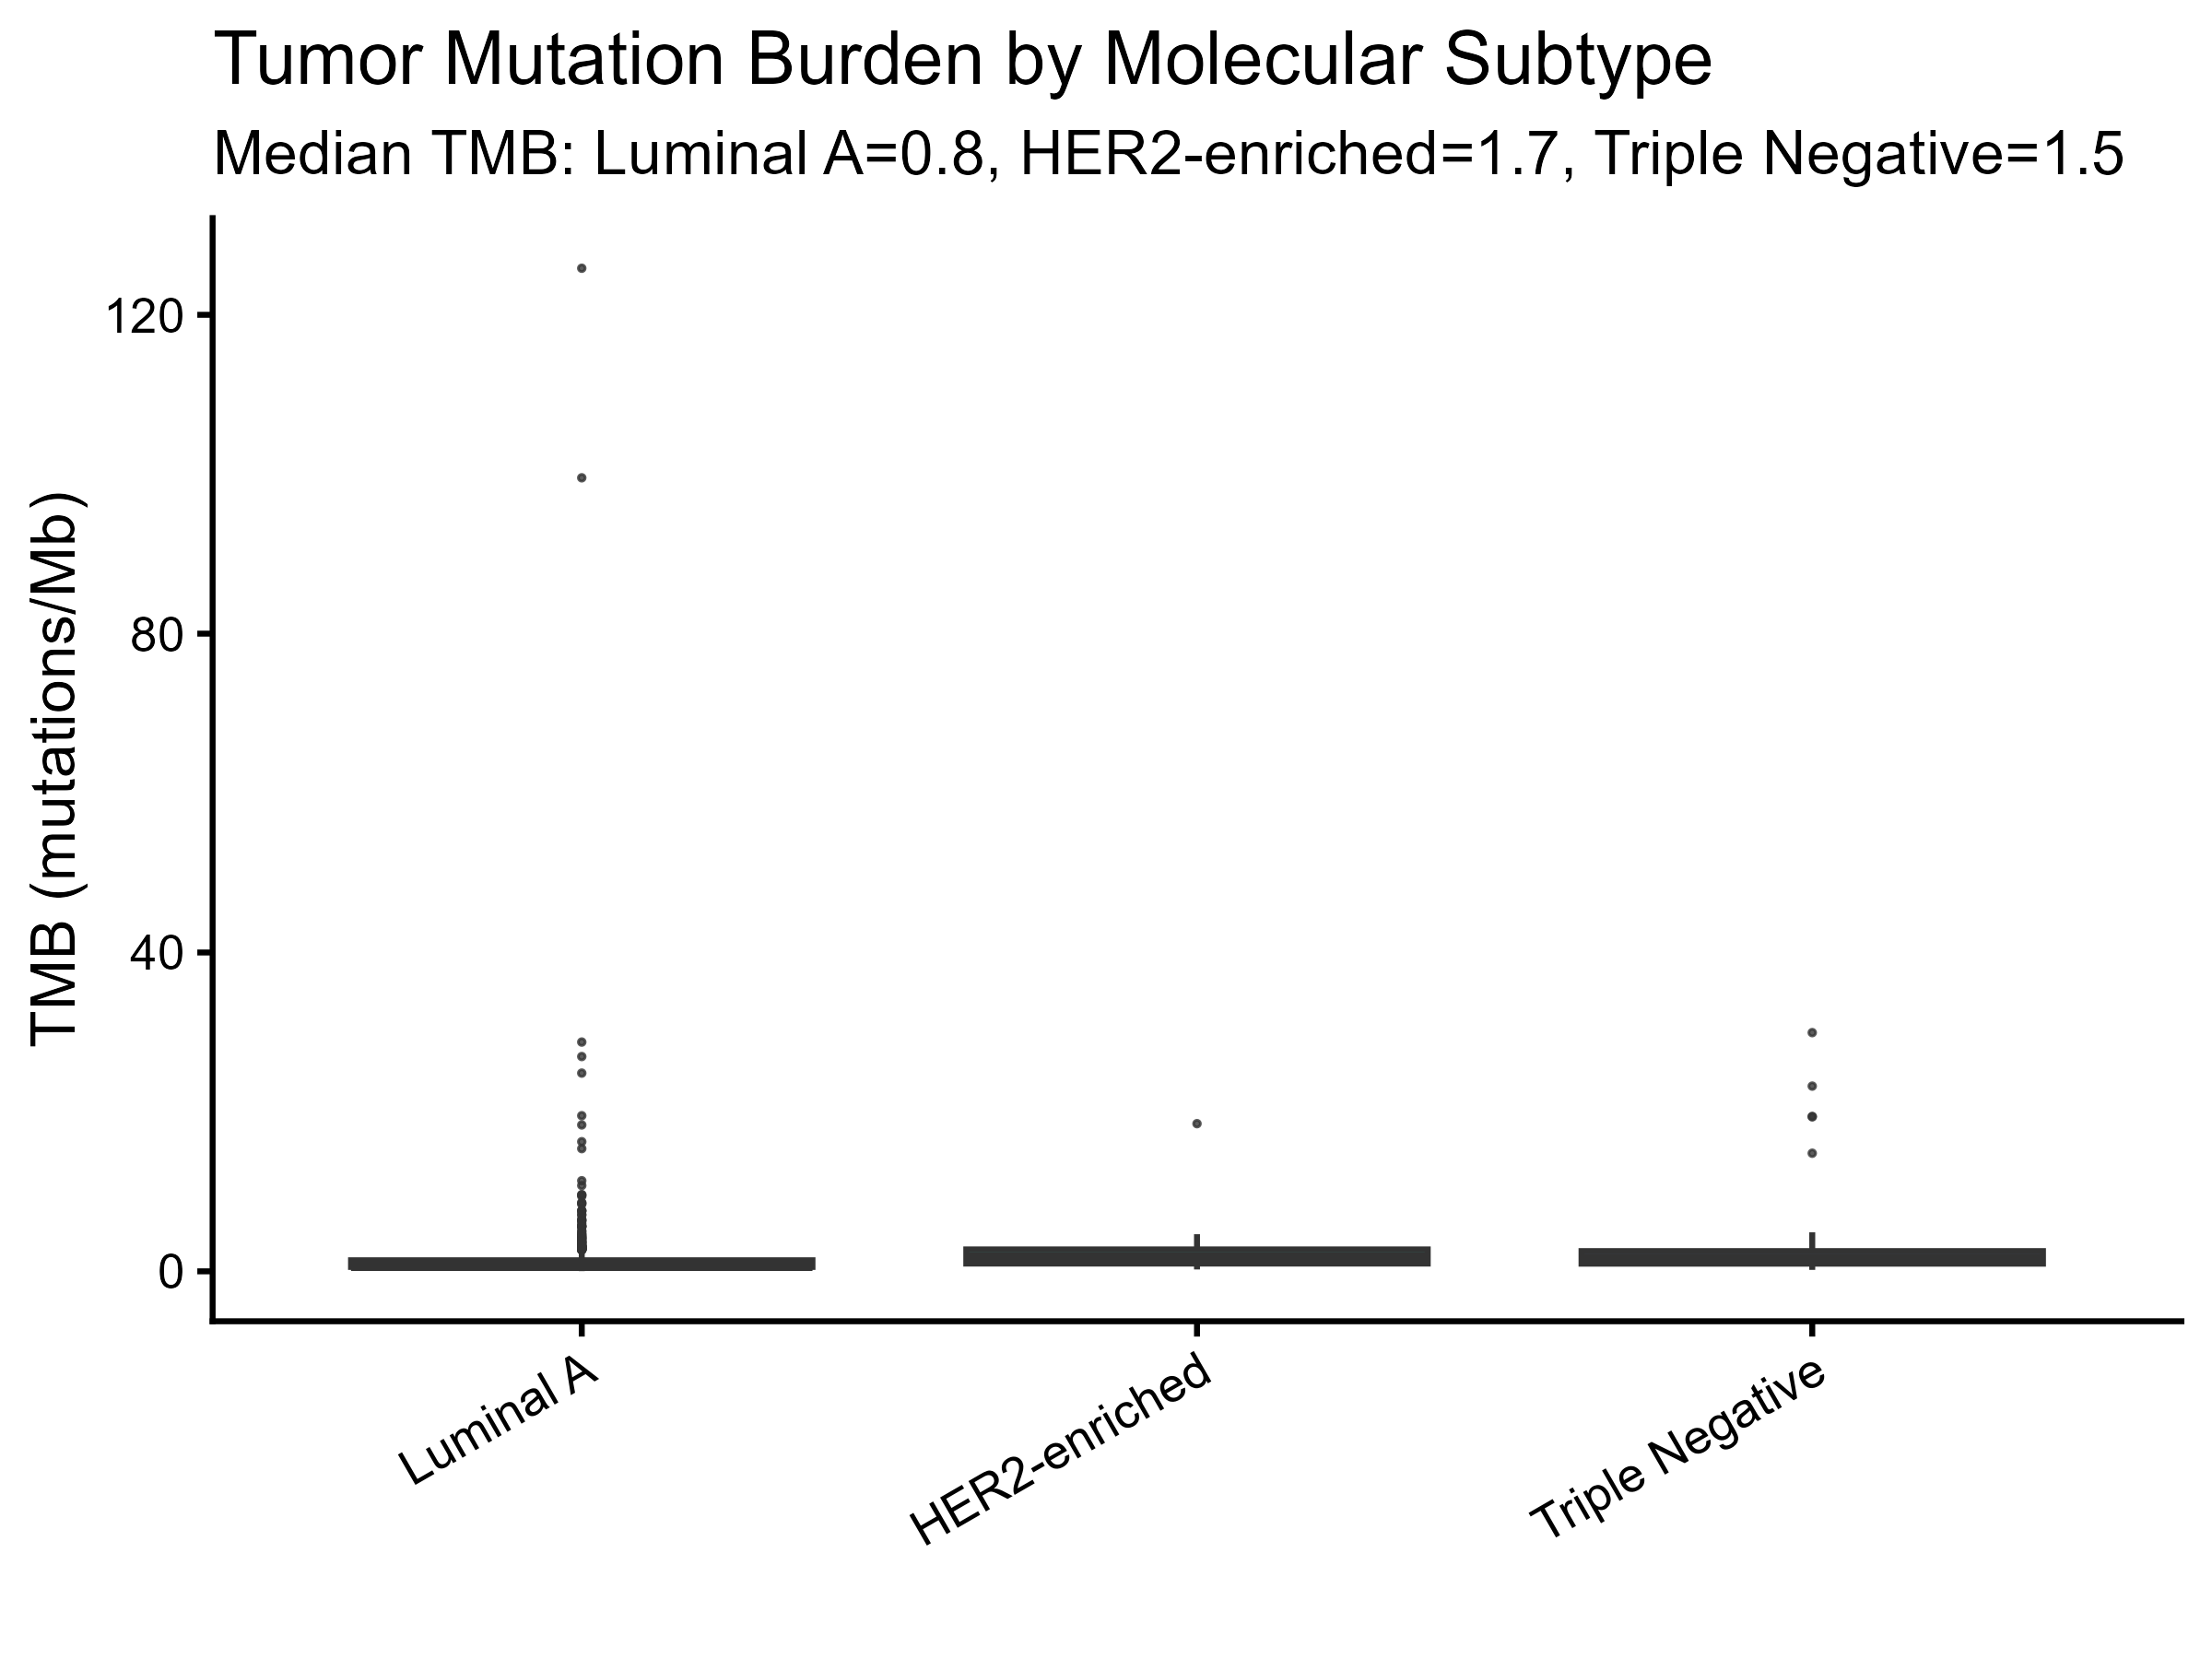
\includegraphics[width=0.85\textwidth]{fig18_tmb_by_subtype.png}
\caption{TMB按分子亚型分布的箱线图。箱体表示IQR，内部横线为中位数，须线延伸至1.5$\times$IQR范围，须外为离群点。TN中位TMB（1.47/Mb）为Luminal A（0.79/Mb）的1.86倍。HER2-enriched因仅35例导致箱体较宽。}
\label{fig:tmb}
\end{figure}

\subsection{关联规则与调控网络}

关联规则散点图（图\ref{fig:rules}）以Support为横轴、Confidence为纵轴、Lift值同时编码点的大小和颜色来展示基因表达—临床特征关联的全局分布。图中每个点代表一条形如\{基因高表达$\rightarrow$特定亚型/受体状态\}的规则。Lift$>1$（暖色调）的点表示基因高表达与特定临床特征之间的共现频率超出了随机期望——这些规则的生物学解释是：该基因在特定亚型中倾向于高表达。位于图中右上角区域的规则兼具高Support（规则覆盖了较多样本）和高Confidence（在满足前提的样本中结论成立的概率高），是最有价值的候选关联。

miRNA-mRNA调控相关性热图（图\ref{fig:mirna}）展示了Top 20 miRNA-mRNA配对（按$|r|$排序）。横轴为mRNA（Gene Symbol），纵轴为miRNA标识，每个格子的颜色由Pearson $r$值编码——从蓝色（负相关，$r\approx-0.6$）经白色（$r\approx0$）渐变至红色（正相关，$r\approx0.6$），格子内标注具体$r$值。以$|r|>0.4$为阈值，在全部miRNA-mRNA配对中共识别2,065对显著调控关系对。图中蓝色格（负相关）占主导，符合miRNA通过碱基配对抑制靶mRNA表达的经典调控机制——miRNA高表达$\rightarrow$靶mRNA低表达，因此相关系数为负。偶见的红色格（正相关）则可能反映了间接调控或共表达效应，而非直接的miRNA-target物理互作。需要指出这些关系均基于统计相关，独立实验验证是确定因果方向的必要条件。

\begin{figure}[H]
\centering
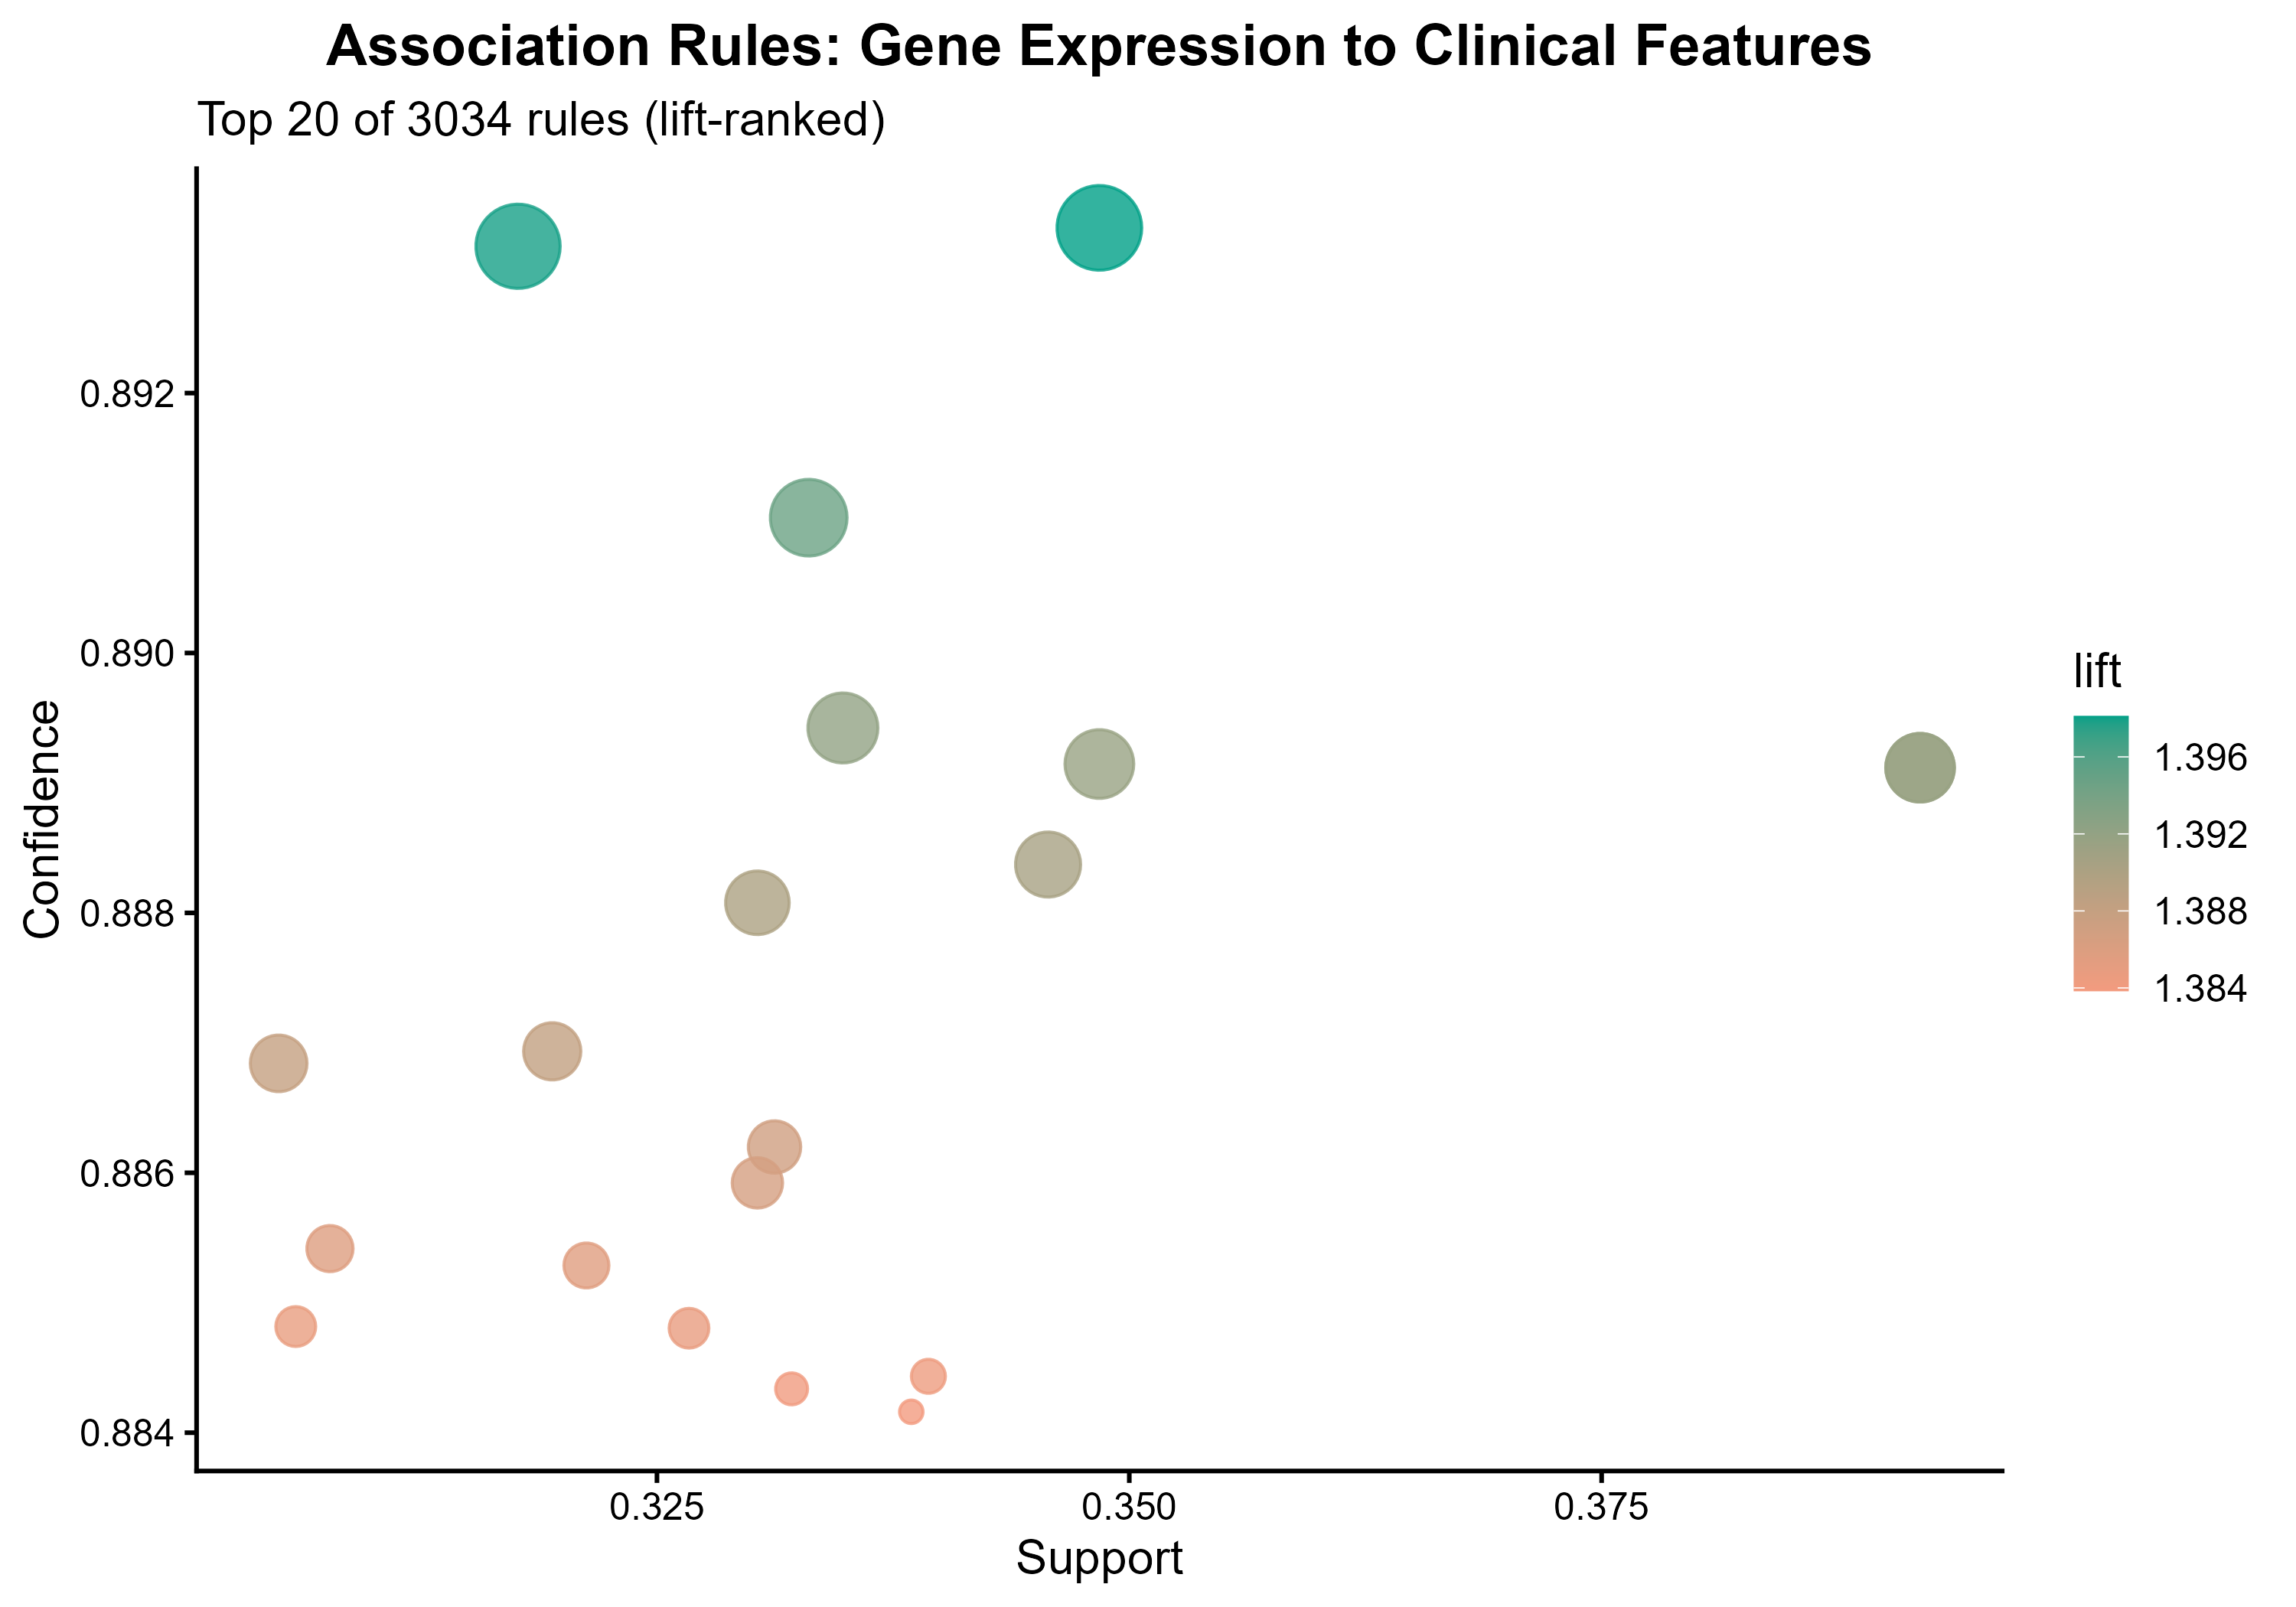
\includegraphics[width=0.8\textwidth]{fig15_association_rules.png}
\caption{关联规则散点图。横轴为Support（规则覆盖比例），纵轴为Confidence（条件概率），点的大小和颜色均编码Lift（$>1$=正关联）。右上角区域的规则兼具高Support和高Confidence，为最可靠的基因—临床特征关联。}
\label{fig:rules}
\end{figure}

\begin{figure}[H]
\centering
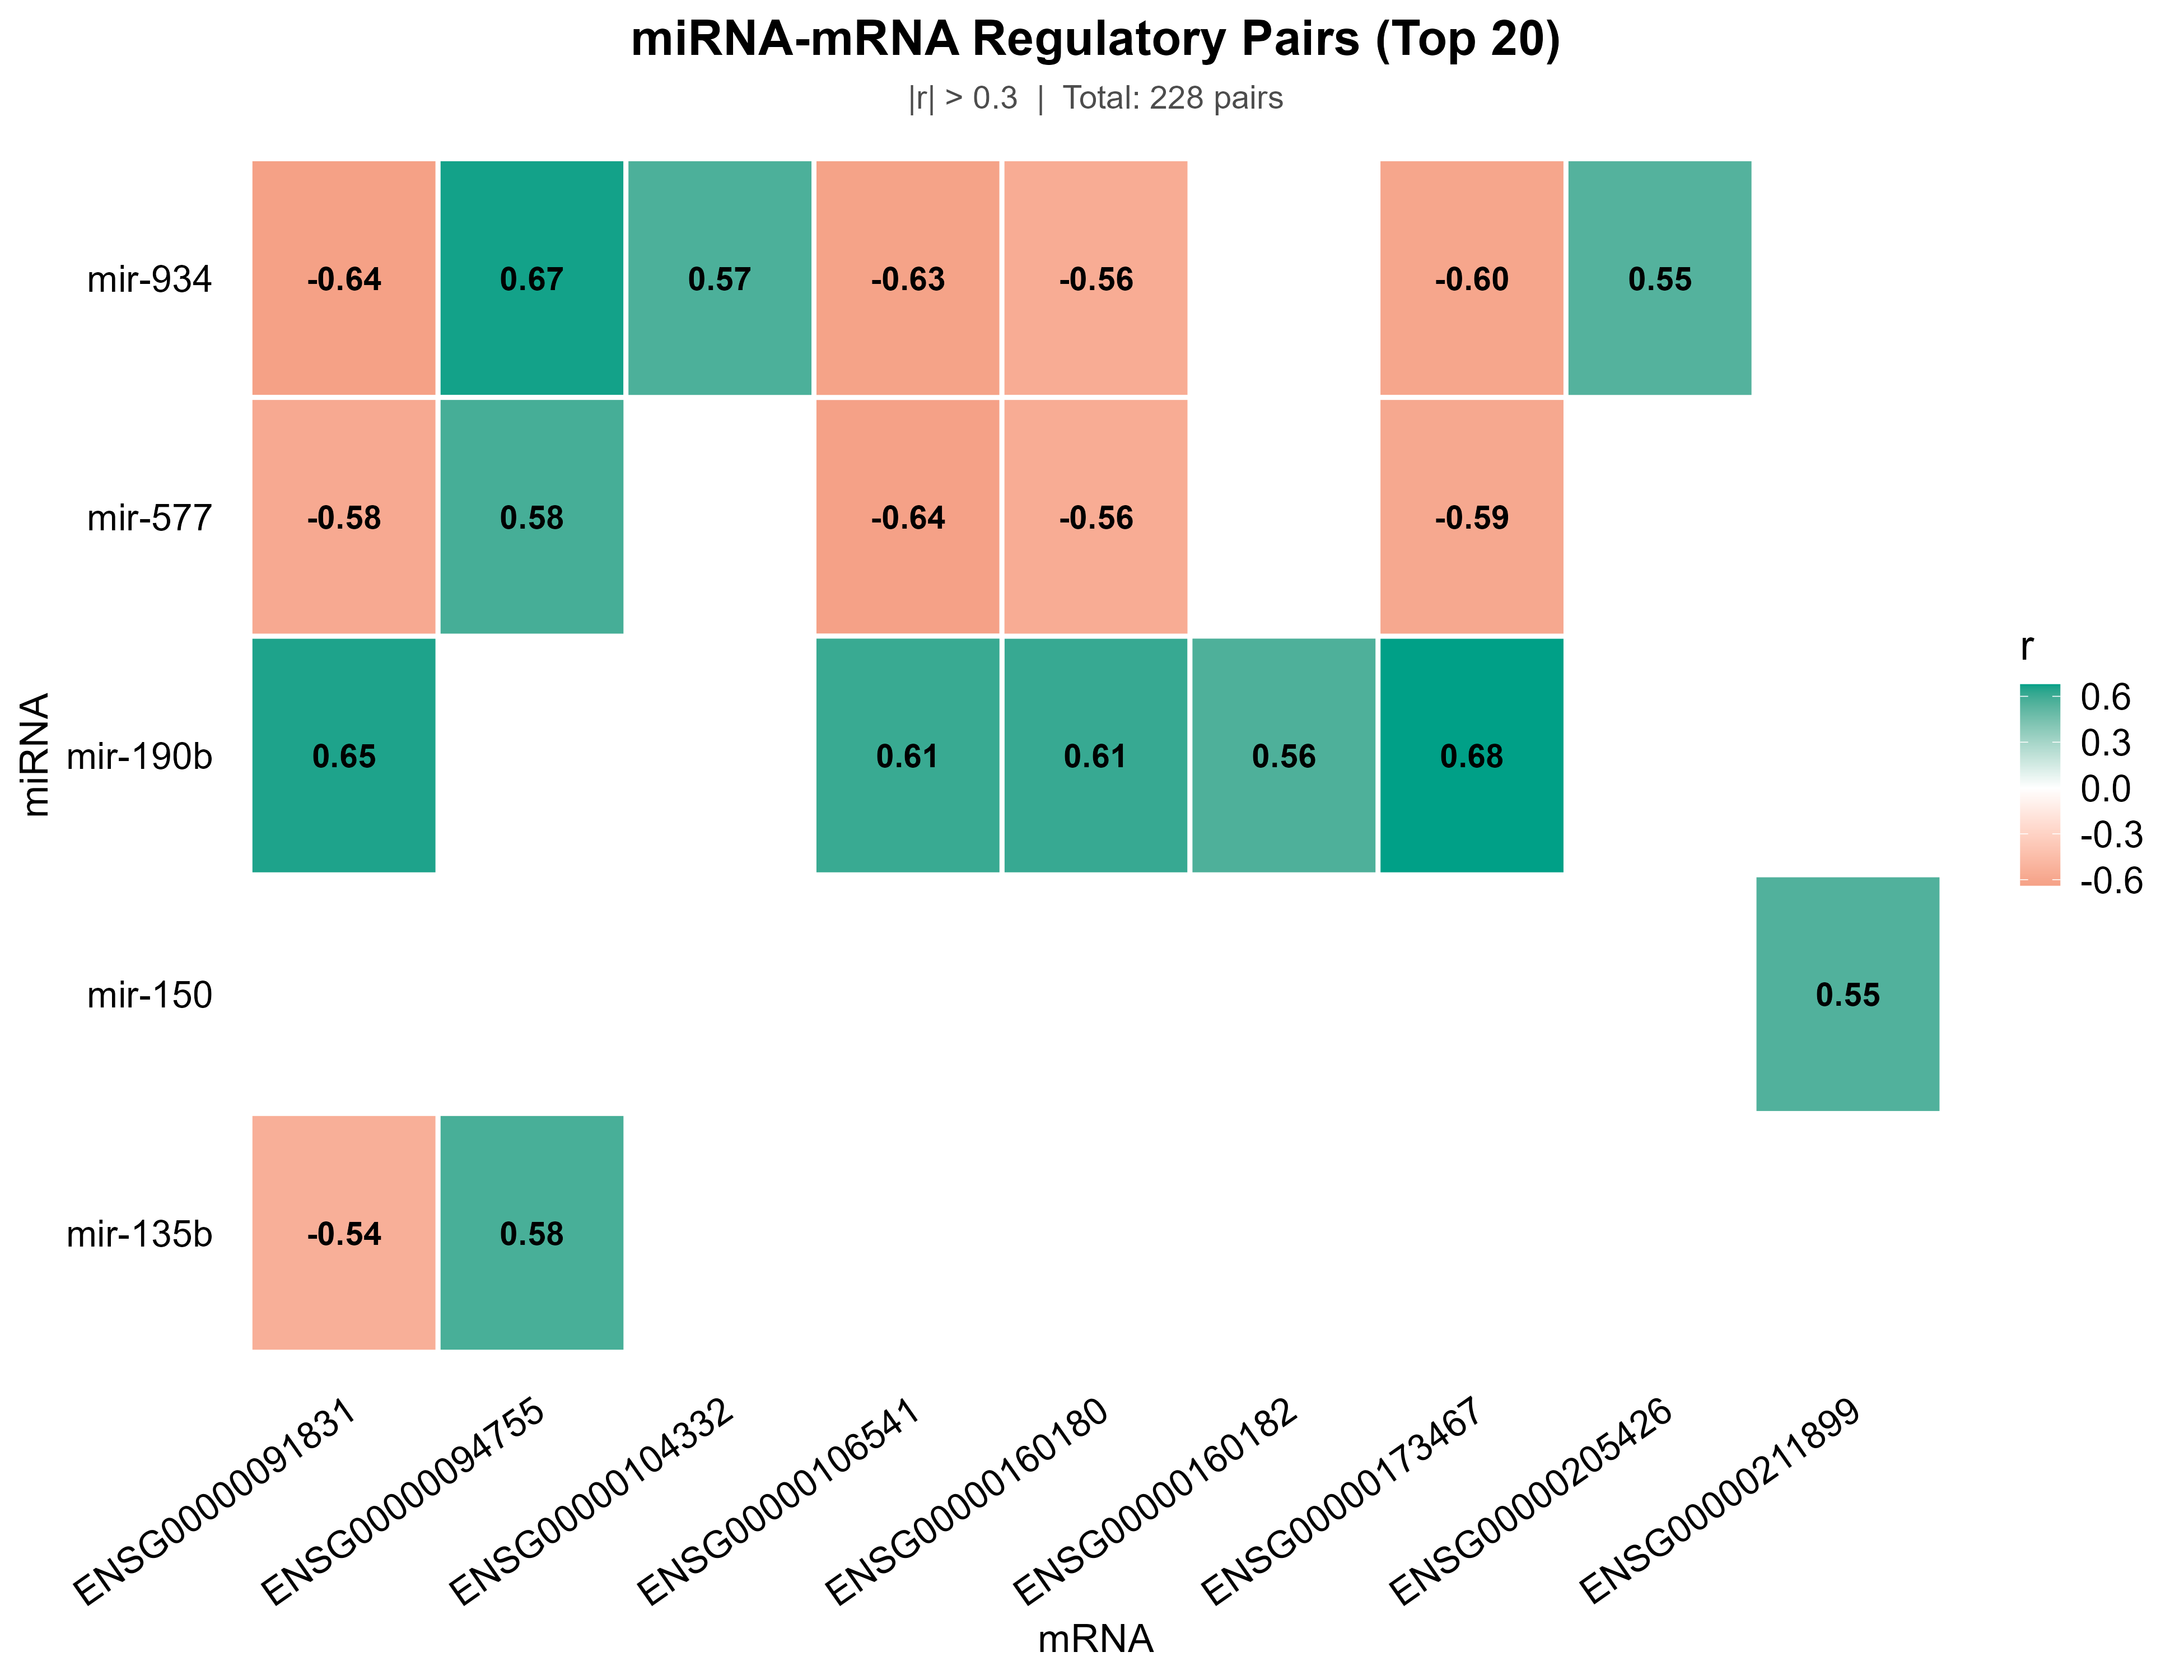
\includegraphics[width=0.85\textwidth]{fig10_mirna_mrna_corr.png}
\caption{miRNA-mRNA调控相关性热图（Top 20, $|r|>0.4$）。行=miRNA, 列=mRNA, 格内标注Pearson $r$值。红-白-蓝色阶：红色=正相关, 白色=无相关, 蓝色=负相关。蓝色格占主导, 符合miRNA抑制靶mRNA的调控预期。}
\label{fig:mirna}
\end{figure}

% ==================== 4 讨论 ====================
\section{讨论}

本研究通过系统的多组学数据挖掘，构建了覆盖11种分析方法的BRCA分子特征整合分析管线。以下从几个关键维度对结果进行讨论。

\textbf{差异表达与功能富集}：上调基因集中于细胞周期和DNA复制通路，下调基因集中于ECM组织和细胞黏附通路——这一功能分工与肿瘤的增殖活跃和微环境脱离特征高度吻合。Reactome Cell Cycle通路的富集显著性（$p=1.5\times10^{-21}$）远超其他通路，反映出细胞周期失调在BRCA转录组全局变化中的核心地位。TN与Luminal A之间存在4,888个差异表达基因，这一数字与Tumor vs Normal的6,768处于同一数量级，暗示亚型间转录组差异的幅度不亚于肿瘤正常差异——对TNBC的靶向治疗开发具有指导意义。

\textbf{分类与聚类的一致性}：LASSO的高准确率（89.4\%）和低特征数（35个基因）共同验证了亚型间转录组差异的稀疏性。PCA、t-SNE和K-means三种独立方法一致指向ER状态为最显著的分组驱动因素，与分类分析中分子亚型的可预测性互为印证。

\textbf{生存预后}：Cox模型在控制分期后分子亚型无独立预后贡献（所有$p>0.5$），与部分文献的结论存在分歧。可能原因：本队列随访时间较短（中位2.7年）、死亡事件有限（87例），以及不同亚型患者接受了针对性治疗部分抹平了固有预后差异。列线图将Cox模型转化为可视化临床工具，3年生存概率可直接从图上读取。

\textbf{突变特征}：PIK3CA和TP53的高频突变及两者互斥趋势与已知BRCA驱动突变谱一致。TMB在Triple Negative中显著高于Luminal A（1.47 vs 0.79/Mb），这一差异具有两方面含义：其一，它可能部分解释了TNBC对免疫检查点抑制剂的较高应答率（更高TMB $\rightarrow$ 更多新抗原 $\rightarrow$ 增强的抗肿瘤免疫）；其二，TMB作为潜在的生物标志物在BRCA亚型分层中的价值值得进一步评估，尽管绝对值低于黑色素瘤和肺癌等典型高TMB癌种。

\textbf{局限性}：（1）DNA甲基化数据（450K, 11.7 GB）未纳入分析；（2）生存事件率较低（7.9\%）限制了预后模型统计功效；（3）miRNA-mRNA调控基于相关而非因果验证；（4）XGBoost未经系统超参数调优，该结果不反映梯度提升方法的理论上限。

% ==================== 5 结论 ====================
\section{结论}

本研究以TCGA-BRCA多组学数据为基础，整合mRNA、miRNA和体细胞突变三个组学层次，构建了覆盖差异表达分析、功能富集、分子亚型分类、聚类分析、WGCNA共表达网络、生存分析、突变分析、关联规则挖掘和miRNA调控网络分析的完整数据挖掘流程。主要结论如下：

（1）鉴定6,768个Tumor vs Normal及4,888个TN vs Luminal A差异表达基因。功能富集揭示上调基因集中于细胞周期通路（$p=1.5\times10^{-21}$），下调基因集中于ECM组织通路。

（2）LASSO以89.4\%准确率仅用35个基因实现三分类分子亚型预测，验证了亚型间转录组差异的稀疏性。

（3）PCA和K-means一致表明ER状态是BRCA转录组的最强驱动因素。

（4）WGCNA识别9个共表达模块，Blue模块枢纽基因MM达0.959。

（5）Cox模型C-index=0.771，Stage IV HR=8.74。列线图提供临床实用预后评估工具。

（6）PIK3CA（37.3\%）和TP53（35.2\%）为最高频突变基因。TN的TMB为Luminal A的1.86倍。

未来方向：纳入DNA甲基化数据实现四组学整合、独立队列外部验证、Blue模块枢纽基因功能实验、以及深度学习方法在多组学数据融合中的应用探索。

% ==================== 参考文献 ====================
\printbibliography

% ==================== 附录 ====================
\newpage
\appendix
\section{核心R代码}

以下附录收录本研究中全部关键分析步骤的R代码。完整项目代码（28个脚本）见项目code/目录。


\subsection{01_data_preprocessing}

\begin{lstlisting}[caption={01_data_preprocessing}, basicstyle=\ttfamily\scriptsize]
# ===========================================================================
# 模块1：BRCA数据预处理
# 项目：BRCA深度基因组分析
# 日期：2026-05-14
# 说明：加载TCGA-BRCA表达和临床数据，执行清洗、标准化、缺失值处理
# ===========================================================================

# 0. 环境设置 ===============================================================
Sys.setlocale("LC_ALL", "English")
options(stringsAsFactors = FALSE, timeout = 600)

suppressPackageStartupMessages({
  library(tidyverse)
  library(data.table)
  library(mice)
  library(VIM)
})

cat("\n========== 模块1：BRCA数据预处理 ==========\n\n")

# 路径定义
DATA_DIR    <- "D:/Users/Desktop/RProject/data"
PRIVATE_DIR <- file.path(DATA_DIR, "private_data")
OUTPUT_DIR  <- file.path(DATA_DIR, "processed")
dir.create(OUTPUT_DIR, showWarnings = FALSE, recursive = TRUE)

# ---- 1. 加载私有数据 ----
cat("Step 1: 加载TCGA-BRCA私有数据...\n")

e <- new.env()
load(file.path(PRIVATE_DIR, "brca_exp.Rdata"), envir = e)
counts_raw <- e$brca
rm(e); gc()

e <- new.env()
load(file.path(PRIVATE_DIR, "brca_clinical.Rdata"), envir = e)
clinical_raw <- e$brca_clinical
rm(e); gc()

cat(sprintf("  表达矩阵: %d 基因 x %d 样本\n", nrow(counts_raw), ncol(counts_raw)))
cat(sprintf("  临床数据: %d 患者 x %d 临床变量\n", nrow(clinical_raw), ncol(clinical_raw)))
cat(sprintf("  数据类型: %s (范围 %.0f - %.0f)\n", typeof(counts_raw), min(counts_raw), max(counts_raw)))

# ---- 2. TCGA Barcode解析 ----
cat("\nStep 2: 解析TCGA barcode，区分肿瘤/正常样本...\n")

barcodes    <- colnames(counts_raw)
patient_ids <- substr(barcodes, 9, 12)
sample_code <- substr(barcodes, 14, 15)

sample_info <- data.frame(
  barcode     = barcodes,
  patient_id  = patient_ids,
  sample_code = sample_code,
  sample_type = case_when(
    sample_code == "01" ~ "Tumor",
    sample_code == "06" ~ "Metastatic",
    sample_code == "11" ~ "Normal",
    TRUE                 ~ "Other"
  ),
  stringsAsFactors = FALSE
)

cat(sprintf("  样本分布: %s\n", paste(names(table(sample_info$sample_type)), 
                                   table(sample_info$sample_type), sep="=", collapse=", ")))
write.csv(sample_info, file.path(OUTPUT_DIR, "sample_info.csv"), row.names = FALSE)

# ---- 3. 拆分肿瘤/正常样本矩阵 ----
cat("\nStep 3: 拆分肿瘤/正常表达矩阵...\n")

tumor_idx   <- which(sample_info$sample_type == "Tumor")
normal_idx  <- which(sample_info$sample_type == "Normal")

counts_tumor  <- counts_raw[, tumor_idx, drop = FALSE]
counts_normal <- counts_raw[, normal_idx, drop = FALSE]

cat(sprintf("  肿瘤样本: %d, 正常样本: %d\n", ncol(counts_tumor), ncol(counts_normal)))

# ---- 4. 低表达基因过滤 ----
cat("\nStep 4: 过滤低表达基因...\n")

min_samples <- max(2, ceiling(ncol(counts_tumor) * 0.1))
keep_genes  <- rowSums(counts_tumor >= 10) >= min_samples

counts_tumor  <- counts_tumor[keep_genes, , drop = FALSE]
counts_normal <- counts_normal[keep_genes, , drop = FALSE]
counts_raw    <- counts_raw[keep_genes, , drop = FALSE]

cat(sprintf("  过滤前基因: %d, 过滤后: %d (保留 %.1f%%)\n", 
            length(keep_genes), sum(keep_genes), 100 * mean(keep_genes)))

# ---- 5. ENSEMBL注释下载 (一次性获取基因symbol+位置) ----
cat("\nStep 5: 下载Ensembl基因注释 (symbol + 基因长度)...\n")

ensembl_ids   <- rownames(counts_tumor)
ensembl_clean <- gsub("\\.\\d+$", "", ensembl_ids)
cat(sprintf("  共 %d 个ENSEMBL基因ID\n", length(ensembl_clean)))

gene_map_file <- file.path(OUTPUT_DIR, "ensembl_gene_map.rds")

if (file.exists(gene_map_file)) {
  cat("  从本地缓存加载基因注释...\n")
  gene_map <- readRDS(gene_map_file)
} else {
  ftp_url <- "https://ftp.ensembl.org/pub/current_tsv/homo_sapiens/Homo_sapiens.GRCh38.113.gene.txt.gz"
  cat(sprintf("  下载Ensembl基因注释: %s\n", ftp_url))
  
  tmp_gz <- tempfile(fileext = ".gz")
  success <- tryCatch({
    download.file(ftp_url, tmp_gz, mode = "wb", timeout = 600)
    TRUE
  }, error = function(e) { FALSE })
  
  if (success) {
    gene_data <- read.table(gzfile(tmp_gz), header = TRUE, sep = "\t",
                            quote = "", comment.char = "", stringsAsFactors = FALSE,
                            fill = TRUE, na.strings = "")
    unlink(tmp_gz)
    
    # 提取: gene_stable_id, gene_name, gene_biotype, description, start, end
    avail_cols <- intersect(c("gene_stable_id", "gene_name", "gene_biotype", 
                               "description", "start_position", "end_position"),
                            colnames(gene_data))
    gene_map <- gene_data[, avail_cols]
    
    # 计算基因长度
    if (all(c("start_position", "end_position") %in% avail_cols)) {
      gene_map$gene_length <- gene_map$end_position - gene_map$start_position + 1
    }
    
    saveRDS(gene_map, gene_map_file)
    cat(sprintf("  下载完成: %d个基因注释\n", nrow(gene_map)))
  } else {
    cat("  Ensembl下载失败，使用备用方案\n")
    gene_map <- data.frame(
      gene_stable_id = ensembl_clean,
      gene_name = ensembl_clean,
      gene_biotype = "unknown",
      description = "unknown",
      gene_length = 1000,
      stringsAsFactors = FALSE
    )
  }
}

# ---- 6. 基因名称和长度赋值 ----
cat("\nStep 6: 基因名称和长度赋值...\n")

# 构建映射：ensembl_clean → symbol
map_idx <- match(ensembl_clean, gene_map$gene_stable_id)

gene_symbol <- ifelse(!is.na(map_idx) & gene_map$gene_name[map_idx] != "",
                      gene_map$gene_name[map_idx], ensembl_ids)
# 处理缺失
gene_symbol[is.na(gene_symbol) | gene_symbol == ""] <- ensembl_ids[is.na(gene_symbol) | gene_symbol == ""]
# 处理重复symbol
dup_idx <- which(duplicated(gene_symbol) | duplicated(gene_symbol, fromLast = TRUE))
gene_symbol[dup_idx] <- paste0(gene_symbol[dup_idx], "_", ensembl_clean[dup_idx])

gene_length_vec <- if ("gene_length" %in% colnames(gene_map) && !is.null(map_idx)) {
  len <- gene_map$gene_length[map_idx]
  len[is.na(len) | len <= 0] <- median(len[!is.na(len) & len > 0], na.rm = TRUE)
  if (all(is.na(len))) len <- rep(1000, length(len))
  len
} else {
  rep(1000, nrow(counts_tumor))
}

cat(sprintf("  有效基因长度: %d (中位数: %.0f bp)\n",
            sum(gene_length_vec > 0), median(gene_length_vec, na.rm = TRUE)))
cat(sprintf("  唯一基因symbol: %d\n", length(unique(gene_symbol))))

# 为矩阵设置行名
rownames(counts_tumor)  <- gene_symbol
rownames(counts_normal) <- gene_symbol
rownames(counts_raw)    <- gene_symbol

# 构建基因注释表
gene_anno <- data.frame(
  ensembl_id      = ensembl_ids,
  ensembl_clean   = ensembl_clean,
  gene_symbol     = gene_symbol,
  gene_length     = gene_length_vec,
  gene_biotype    = ifelse(!is.na(map_idx), gene_map$gene_biotype[map_idx], "unknown"),
  description     = ifelse(!is.na(map_idx), gene_map$description[map_idx], "unknown"),
  stringsAsFactors = FALSE
)

# ---- 7. Counts → TPM 标准化 ----
cat("\nStep 7: Counts → TPM标准化...\n")

counts_to_tpm <- function(counts, gene_lengths) {
  rpk <- counts / (gene_lengths / 1000)
  sweep(rpk, 2, colSums(rpk) / 1e6, "/")
}

tpm_tumor  <- counts_to_tpm(counts_tumor, gene_length_vec)
tpm_normal <- counts_to_tpm(counts_normal, gene_length_vec)

cat(sprintf("  TPM完成 (log2范围: 肿瘤 %.2f-%.2f, 正常 %.2f-%.2f)\n",
            min(log2(tpm_tumor + 1)), max(log2(tpm_tumor + 1)),
            min(log2(tpm_normal + 1)), max(log2(tpm_normal + 1))))

# ---- 8. 临床数据清洗 ----
cat("\nStep 8: 临床数据清洗与变量提取...\n")

# 提取关键临床变量
key_vars <- c("bcr_patient_barcode", "vital_status", "days_to_death",
              "days_to_last_followup", "age_at_initial_pathologic_diagnosis",
              "gender", "race_list", "stage_event_pathologic_stage",
              "stage_event_tnm_categories",
              "breast_carcinoma_estrogen_receptor_status",
              "breast_carcinoma_progesterone_receptor_status",
              "lab_proc_her2_neu_immunohistochemistry_receptor_status",
              "histological_type", "menopause_status",
              "person_neoplasm_cancer_status",
              "number_of_lymphnodes_positive_by_he",
              "radiation_therapy", "postoperative_rx_tx")

clinical <- clinical_raw[, intersect(key_vars, colnames(clinical_raw)), drop = FALSE]

# 重命名
name_map <- c(
  "bcr_patient_barcode" = "patient_id",
  "vital_status" = "vital_status",
  "days_to_death" = "days_to_death",
  "days_to_last_followup" = "days_to_last_followup",
  "age_at_initial_pathologic_diagnosis" = "age_at_diagnosis",
  "gender" = "gender",
  "race_list" = "race",
  "stage_event_pathologic_stage" = "pathologic_stage",
  "stage_event_tnm_categories" = "tnm_categories",
  "breast_carcinoma_estrogen_receptor_status" = "er_status",
  "breast_carcinoma_progesterone_receptor_status" = "pr_status",
  "lab_proc_her2_neu_immunohistochemistry_receptor_status" = "her2_status",
  "histological_type" = "histological_type",
  "menopause_status" = "menopause_status",
  "person_neoplasm_cancer_status" = "cancer_status",
  "number_of_lymphnodes_positive_by_he" = "positive_lymph_nodes",
  "radiation_therapy" = "radiation_therapy",
  "postoperative_rx_tx" = "postoperative_rx"
)
for (nm in intersect(names(name_map), colnames(clinical))) {
  colnames(clinical)[colnames(clinical) == nm] <- name_map[nm]
}

# 计算OS和生存事件
clinical <- clinical %>%
  mutate(
    vital_status = ifelse(vital_status == "Dead", 1, 0),
    os_time = ifelse(vital_status == 1,
                     as.numeric(days_to_death),
                     as.numeric(days_to_last_followup)),
    os_time = ifelse(os_time <= 0 | is.na(os_time), 1, os_time)
  )

# 简化病理分期
clinical <- clinical %>%
  mutate(
    stage_simple = case_when(
      grepl("Stage I[A-C]?$|Stage I$", pathologic_stage, ignore.case = TRUE) ~ "Stage I",
      grepl("Stage II[A-C]?$|Stage II$", pathologic_stage, ignore.case = TRUE) ~ "Stage II",
      grepl("Stage III[A-C]?$|Stage III$", pathologic_stage, ignore.case = TRUE) ~ "Stage III",
      grepl("Stage IV[A-C]?$|Stage IV$", pathologic_stage, ignore.case = TRUE) ~ "Stage IV",
      TRUE ~ NA_character_
    )
  )

# 分子亚型分类
clinical <- clinical %>%
  mutate(
    er_status_clean = case_when(
      grepl("Positive", er_status, ignore.case = TRUE) ~ "Positive",
      grepl("Negative", er_status, ignore.case = TRUE) ~ "Negative",
      TRUE ~ NA_character_
    ),
    pr_status_clean = case_when(
      grepl("Positive", pr_status, ignore.case = TRUE) ~ "Positive",
      grepl("Negative", pr_status, ignore.case = TRUE) ~ "Negative",
      TRUE ~ NA_character_
    ),
    her2_status_clean = case_when(
      grepl("Positive", her2_status, ignore.case = TRUE) ~ "Positive",
      grepl("Negative", her2_status, ignore.case = TRUE) ~ "Negative",
      grepl("Equivocal|Indeterminate", her2_status, ignore.case = TRUE) ~ "Equivocal",
      TRUE ~ NA_character_
    ),
    molecular_subtype = case_when(
      (er_status_clean == "Positive" | pr_status_clean == "Positive") & her2_status_clean == "Negative" ~ "Luminal A",
      (er_status_clean == "Positive" | pr_status_clean == "Positive") & her2_status_clean == "Positive" ~ "Luminal B",
      er_status_clean == "Negative" & pr_status_clean == "Negative" & her2_status_clean == "Positive" ~ "HER2-enriched",
      er_status_clean == "Negative" & pr_status_clean == "Negative" & her2_status_clean == "Negative" ~ "Triple Negative",
      TRUE ~ NA_character_
    )
  )

cat(sprintf("  提取 %d 个关键临床变量\n", ncol(clinical)))

# ---- 9. 缺失值处理 ----
cat("\nStep 9: 缺失值处理...\n")

impute_cols <- c("age_at_diagnosis", "positive_lymph_nodes", "os_time",
                 "stage_simple", "molecular_subtype", "race")

impute_cols <- intersect(impute_cols, colnames(clinical))

for (v in names(clinical)) {
  miss_n <- sum(is.na(clinical[[v]]))
  if (miss_n > 0) cat(sprintf("    %-25s: %d (%.1f%%)\n", v, miss_n, 100*miss_n/nrow(clinical)))
}

# 简单中位数/众数填充
for (v in intersect(impute_cols, colnames(clinical))) {
  nas <- is.na(clinical[[v]])
  if (any(nas)) {
    if (is.numeric(clinical[[v]])) {
      clinical[[v]][nas] <- median(clinical[[v]], na.rm = TRUE)
    } else {
      tbl <- table(clinical[[v]])
      clinical[[v]][nas] <- names(tbl)[which.max(tbl)]
    }
  }
}
cat("  缺失值填充完成\n")

# ---- 10. 临床-表达对齐 ----
cat("\nStep 10: 临床-表达样本对齐...\n")

expr_patients_id <- substr(colnames(counts_tumor), 9, 12)
clinical$patient_id_short <- gsub("^TCGA-\\w{2}-", "", clinical$patient_id)

match_idx <- match(expr_patients_id, clinical$patient_id_short)
matched   <- !is.na(match_idx)

counts_tumor_final  <- counts_tumor[, matched, drop = FALSE]
tpm_tumor_final     <- tpm_tumor[, matched, drop = FALSE]
clinical_final      <- clinical[match_idx[matched], , drop = FALSE]

cat(sprintf("  匹配: %d / %d (%.1f%%)\n",
            ncol(counts_tumor_final), ncol(counts_tumor), 100 * mean(matched)))

# ---- 11. 保存数据 ----
cat("\nStep 11: 保存处理后数据...\n")

saveRDS(counts_tumor_final, file.path(OUTPUT_DIR, "brca_tumor_counts.rds"))
saveRDS(tpm_tumor_final, file.path(OUTPUT_DIR, "brca_tumor_tpm.rds"))
saveRDS(clinical_final, file.path(OUTPUT_DIR, "brca_clinical_clean.rds"))
saveRDS(gene_anno, file.path(OUTPUT_DIR, "gene_annotation.rds"))

if (ncol(counts_normal) > 0) {
  saveRDS(counts_normal, file.path(OUTPUT_DIR, "brca_normal_counts.rds"))
  saveRDS(tpm_normal, file.path(OUTPUT_DIR, "brca_normal_tpm.rds"))
}

# 完整打包
saveRDS(list(
  counts           = counts_tumor_final,
  tpm              = tpm_tumor_final,
  clinical         = clinical_final,
  gene_annotation  = gene_anno,
  sample_info      = sample_info,
  preprocessing_date = Sys.time()
), file.path(OUTPUT_DIR, "brca_tumor_processed.rds"))

# ---- 12. 预处理报告 ----
cat("\n========== 预处理完成报告 ==========\n")
cat(sprintf("  输出目录: %s\n", OUTPUT_DIR))
cat(sprintf("  肿瘤样本: %d (表达矩阵 %d基因 x %d样本)\n",
            ncol(counts_tumor_final), nrow(counts_tumor_final), ncol(counts_tumor_final)))
cat(sprintf("  正常样本: %d\n", ncol(counts_normal)))
cat(sprintf("  临床变量: %d\n", ncol(clinical_final)))

if ("stage_simple" %in% colnames(clinical_final)) {
  cat(sprintf("  病理分期: %s\n",
              paste(names(table(clinical_final$stage_simple)),
                    table(clinical_final$stage_simple), sep="=", collapse=", ")))
}
if ("molecular_subtype" %in% colnames(clinical_final)) {
  cat(sprintf("  分子亚型: %s\n",
              paste(names(table(clinical_final$molecular_subtype)),
                    table(clinical_final$molecular_subtype), sep="=", collapse=", ")))
}
cat(sprintf("  生存: 死亡=%d 存活=%d\n",
            sum(clinical_final$vital_status == 1, na.rm = TRUE),
            sum(clinical_final$vital_status == 0, na.rm = TRUE)))
cat("=========================================\n")

# 摘要表
summary_table <- data.frame(
  Metric = c("原始基因数","过滤后基因数","肿瘤样本数","正常样本数",
             "临床变量数","死亡事件","存活",
             "Stage I","Stage II","Stage III","Stage IV",
             "Luminal A","Luminal B","HER2-enriched","Triple Negative"),
  Value = c(
    length(keep_genes), nrow(counts_tumor_final), ncol(counts_tumor_final),
    ncol(counts_normal), ncol(clinical_final),
    sum(clinical_final$vital_status == 1, na.rm = TRUE),
    sum(clinical_final$vital_status == 0, na.rm = TRUE),
    sum(clinical_final$stage_simple == "Stage I", na.rm = TRUE),
    sum(clinical_final$stage_simple == "Stage II", na.rm = TRUE),
    sum(clinical_final$stage_simple == "Stage III", na.rm = TRUE),
    sum(clinical_final$stage_simple == "Stage IV", na.rm = TRUE),
    sum(clinical_final$molecular_subtype == "Luminal A", na.rm = TRUE),
    sum(clinical_final$molecular_subtype == "Luminal B", na.rm = TRUE),
    sum(clinical_final$molecular_subtype == "HER2-enriched", na.rm = TRUE),
    sum(clinical_final$molecular_subtype == "Triple Negative", na.rm = TRUE)
  )
)
write.csv(summary_table, file.path(OUTPUT_DIR, "preprocessing_summary.csv"), row.names = FALSE)

cat("预处理全部完成!\n")
\end{lstlisting}

\subsection{02_download_mirna}

\begin{lstlisting}[caption={02_download_mirna}, basicstyle=\ttfamily\scriptsize]
# ===========================================================================
# US-001: Download BRCA miRNA-seq data from TCGA via TCGAbiolinks
# 项目：BRCA多组学数据挖掘
# 日期：2026-05-14
# ===========================================================================

Sys.setlocale("LC_ALL", "English")
options(stringsAsFactors = FALSE, timeout = 1200)

suppressPackageStartupMessages({
  library(TCGAbiolinks)
  library(SummarizedExperiment)
})

cat("\n========== US-001: Download BRCA miRNA-seq Data ==========\n\n")

OUT_DIR <- "D:/Users/Desktop/R_Work/data/public_data"
dir.create(OUT_DIR, showWarnings = FALSE, recursive = TRUE)

# ---- 1. Query GDC for BRCA miRNA data ----
cat("Step 1: Querying GDC for TCGA-BRCA miRNA-seq data...\n")
cat("  Data Category: Transcriptome Profiling\n")
cat("  Data Type: miRNA Expression Quantification\n")

mirna_query <- GDCquery(
  project       = "TCGA-BRCA",
  data.category = "Transcriptome Profiling",
  data.type     = "miRNA Expression Quantification",
  workflow.type = "BCGSC miRNA Profiling",
  access        = "open"
)

cat(sprintf("  Query returned: %d cases, %d files\n",
            length(unique(mirna_query$results[[1]]$cases)),
            nrow(mirna_query$results[[1]])))

# ---- 2. Download data ----
cat("\nStep 2: Downloading miRNA data from GDC...\n")

GDCdownload(
  query   = mirna_query,
  method  = "api",
  files.per.chunk = 20
)

# ---- 3. Prepare data ----
cat("\nStep 3: Preparing miRNA expression matrix...\n")

mirna_data <- GDCprepare(
  query   = mirna_query,
  save           = TRUE,
  save.filename  = file.path(OUT_DIR, "brca_mirna_se.rds")
)

cat(sprintf("  Data dimensions: %d rows x %d columns\n",
            nrow(mirna_data), ncol(mirna_data)))
cat(sprintf("  Class: %s\n", paste(class(mirna_data), collapse = ", ")))

# ---- 4. Extract count matrix ----
# GDC miRNA data may return data.frame or SummarizedExperiment
cat("\nStep 4: Extracting read count matrix...\n")

if (inherits(mirna_data, "SummarizedExperiment")) {
  mirna_counts <- assay(mirna_data, "read_count")
  if (is.null(mirna_counts)) {
    avail_assays <- assayNames(mirna_data)
    cat(sprintf("  Available assays: %s\n", paste(avail_assays, collapse = ", ")))
    mirna_counts <- assay(mirna_data, 1)
  }
  mirna_clinical <- as.data.frame(colData(mirna_data))
  barcodes <- colnames(mirna_counts)

} else if (is.data.frame(mirna_data)) {
  # Data.frame format: col1=miRNA_ID, then 3 cols per sample (read_count, RPM, cross-mapped)
  cat("  Data is data.frame — extracting read_count columns\n")

  mirna_id_col <- mirna_data[, 1, drop = TRUE]
  all_cols <- colnames(mirna_data)[-1]

  # Each sample has 3 quantification types; extract read_count columns
  read_count_cols <- grep("read_count", all_cols, ignore.case = TRUE, value = TRUE)

  if (length(read_count_cols) == 0) {
    # Alternative: every 3rd column starting from col 2
    sample_cols <- all_cols[seq(1, length(all_cols), by = 3)]
    mirna_counts <- as.matrix(mirna_data[, sample_cols, drop = FALSE])
    colnames(mirna_counts) <- gsub("_read_count|_reads_per_million|_cross.mapped", "", sample_cols)
  } else {
    mirna_counts <- as.matrix(mirna_data[, read_count_cols, drop = FALSE])
    colnames(mirna_counts) <- gsub("_read_count", "", read_count_cols)
  }

  rownames(mirna_counts) <- mirna_id_col

  # Build clinical from barcodes
  barcodes <- colnames(mirna_counts)
  mirna_clinical <- data.frame(
    barcode = barcodes,
    stringsAsFactors = FALSE
  )

} else {
  stop("Unexpected data format from GDCprepare")
}

cat(sprintf("  Count matrix: %d miRNAs x %d samples\n",
            nrow(mirna_counts), ncol(mirna_counts)))

# ---- 5. Parse TCGA barcode ----
cat("\nStep 5: Parsing sample metadata...\n")

sample_code  <- substr(barcodes, 14, 15)
mirna_clinical$sample_type <- ifelse(sample_code == "01", "Tumor",
                              ifelse(sample_code == "11", "Normal", "Other"))
mirna_clinical$patient_id  <- substr(barcodes, 9, 12)

cat(sprintf("  Sample types: %s\n",
            paste(names(table(mirna_clinical$sample_type)),
                  table(mirna_clinical$sample_type), sep = "=", collapse = ", ")))

# ---- 6. Save processed data ----
cat("\nStep 5: Saving processed miRNA data...\n")

saveRDS(mirna_counts, file.path(OUT_DIR, "brca_mirna_counts.rds"))
saveRDS(mirna_clinical, file.path(OUT_DIR, "brca_mirna_clinical.rds"))

cat(sprintf("  Saved: brca_mirna_counts.rds (%d x %d)\n",
            nrow(mirna_counts), ncol(mirna_counts)))
cat(sprintf("  Saved: brca_mirna_clinical.rds (%d x %d)\n",
            nrow(mirna_clinical), ncol(mirna_clinical)))

# ---- 7. Download log ----
log_lines <- c(
  paste("Download date:", Sys.time()),
  paste("Data type: miRNA Expression Quantification"),
  paste("Platform: Illumina HiSeq (BCGSC miRNA Profiling)"),
  paste("Dimensions:", nrow(mirna_counts), "miRNAs x", ncol(mirna_counts), "samples"),
  paste("Sample distribution:", paste(names(table(mirna_clinical$sample_type)),
        table(mirna_clinical$sample_type), sep = "=", collapse = ", ")),
  paste("File size:", round(file.size(file.path(OUT_DIR, "brca_mirna_counts.rds")) / 1024^2, 2), "MB")
)
writeLines(log_lines, file.path(OUT_DIR, "brca_mirna_download_log.txt"))

cat("\n========== US-001 Complete: miRNA Download ==========\n")
\end{lstlisting}

\subsection{02_download_mutations}

\begin{lstlisting}[caption={02_download_mutations}, basicstyle=\ttfamily\scriptsize]
# ===========================================================================
# US-003: Download BRCA Somatic Mutation data from TCGA via TCGAbiolinks
# 项目：BRCA多组学数据挖掘
# 日期：2026-05-14
# ===========================================================================

Sys.setlocale("LC_ALL", "English")
options(stringsAsFactors = FALSE, timeout = 1200)

suppressPackageStartupMessages({
  library(TCGAbiolinks)
  library(maftools)
})

cat("\n========== US-003: Download BRCA Somatic Mutation Data ==========\n\n")

OUT_DIR <- "D:/Users/Desktop/R_Work/data/public_data"
dir.create(OUT_DIR, showWarnings = FALSE, recursive = TRUE)

# ---- 1. Download MAF via GDCquery_Maf ----
cat("Step 1: Downloading TCGA-BRCA MAF (Mutect2 pipeline)...\n")

# Try Mutect2 first, fall back to varscan or muse
maf_file <- file.path(OUT_DIR, "brca_mutations.maf")
rds_file <- file.path(OUT_DIR, "brca_mutations.rds")

maf_download_success <- FALSE

tryCatch({
  maf_query <- GDCquery_Maf(
    tumor     = "BRCA",
    pipelines = "mutect2",
    save.csv  = TRUE,
    directory = OUT_DIR
  )
  maf_download_success <- TRUE
  cat("  Successfully downloaded Mutect2 MAF\n")
}, error = function(e) {
  cat(sprintf("  Mutect2 failed: %s\n", e$message))
  cat("  Trying varscan2 pipeline...\n")
  tryCatch({
    maf_query <<- GDCquery_Maf(
      tumor     = "BRCA",
      pipelines = "varscan2",
      save.csv  = TRUE,
      directory = OUT_DIR
    )
    maf_download_success <<- TRUE
    cat("  Successfully downloaded varscan2 MAF\n")
  }, error = function(e2) {
    cat(sprintf("  varscan2 also failed: %s\n", e2$message))
    cat("  Trying muse pipeline...\n")
    tryCatch({
      maf_query <<- GDCquery_Maf(
        tumor     = "BRCA",
        pipelines = "muse",
        save.csv  = TRUE,
        directory = OUT_DIR
      )
      maf_download_success <<- TRUE
      cat("  Successfully downloaded muse MAF\n")
    }, error = function(e3) {
      cat(sprintf("  All pipelines failed: %s\n", e3$message))
    })
  })
})

# ---- 2. If direct MAF download failed, try GDCquery approach ----
if (!maf_download_success) {
  cat("\nStep 1b: Trying alternative GDCquery approach for mutations...\n")

  tryCatch({
    mut_query <- GDCquery(
      project       = "TCGA-BRCA",
      data.category = "Simple Nucleotide Variation",
      data.type     = "Masked Somatic Mutation",
      workflow.type = "Aliquot Ensemble Somatic Variant Merging and Masking",
      access        = "open"
    )

    if (nrow(mut_query$results[[1]]) > 0) {
      cat(sprintf("  Found %d mutation files\n", nrow(mut_query$results[[1]])))

      GDCdownload(mut_query, method = "api", files.per.chunk = 20)

      maf_data <- GDCprepare(mut_query)
      saveRDS(maf_data, rds_file)

      cat(sprintf("  Mutation data saved: %d variants\n", nrow(maf_data)))
      maf_download_success <- TRUE
    }
  }, error = function(e) {
    cat(sprintf("  Alternative approach also failed: %s\n", e$message))
  })
}

# ---- 3. Process MAF with maftools ----
if (maf_download_success && exists("maf_query")) {
  cat("\nStep 2: Processing MAF with maftools...\n")

  maf <- read.maf(
    maf     = maf_query,
    verbose = TRUE
  )

  cat(sprintf("  MAF summary: %d samples, %d genes, %d variants\n",
              length(unique(maf@data$Tumor_Sample_Barcode)),
              length(unique(maf@data$Hugo_Symbol)),
              nrow(maf@data)))

  # Save as RDS for easy loading
  saveRDS(maf, rds_file)

  # ---- 4. Mutation summary statistics ----
  cat("\nStep 3: Computing mutation summary statistics...\n")

  # Top mutated genes
  gene_summary <- maf@data %>%
    dplyr::count(Hugo_Symbol, sort = TRUE) %>%
    dplyr::rename(N_Mutations = n)

  cat(sprintf("  Top 10 mutated genes:\n"))
  for (i in 1:min(10, nrow(gene_summary))) {
    cat(sprintf("    %s: %d mutations\n", gene_summary$Hugo_Symbol[i],
                gene_summary$N_Mutations[i]))
  }

  # Variant type distribution
  var_summary <- maf@data %>%
    dplyr::count(Variant_Classification, sort = TRUE)
  cat(sprintf("\n  Variant types:\n"))
  for (i in 1:min(8, nrow(var_summary))) {
    cat(sprintf("    %s: %d (%.1f%%)\n", var_summary$Variant_Classification[i],
                var_summary$n[i], 100 * var_summary$n[i] / sum(var_summary$n)))
  }

  # Variant type distribution table
  write.csv(var_summary, file.path(OUT_DIR, "brca_variant_types.csv"), row.names = FALSE)
  write.csv(gene_summary, file.path(OUT_DIR, "brca_mutated_genes.csv"), row.names = FALSE)

  # ---- 5. Download log ----
  log_lines <- c(
    paste("Download date:", Sys.time()),
    paste("Data type: Somatic Mutation (MAF format)"),
    paste("Pipeline: Mutect2 / Varscan2 / Muse"),
    paste("Samples:", length(unique(maf@data$Tumor_Sample_Barcode))),
    paste("Genes mutated:", length(unique(maf@data$Hugo_Symbol))),
    paste("Total variants:", nrow(maf@data)),
    paste("Top mutated gene:", gene_summary$Hugo_Symbol[1],
          sprintf("(%d mutations)", gene_summary$N_Mutations[1]))
  )
  writeLines(log_lines, file.path(OUT_DIR, "brca_mutation_download_log.txt"))

} else {
  cat("\nWARNING: MAF data could not be downloaded or processed.\n")
  cat("Will proceed with available data in integration step.\n")

  log_lines <- c(
    paste("Download date:", Sys.time()),
    "Status: FAILED - No MAF data could be retrieved",
    "Note: Mutation analysis will be skipped or use alternative source"
  )
  writeLines(log_lines, file.path(OUT_DIR, "brca_mutation_download_log.txt"))
}

cat("\n========== US-003 Complete: Mutation Download ==========\n")
\end{lstlisting}

\subsection{03_integrate_omics}

\begin{lstlisting}[caption={03_integrate_omics}, basicstyle=\ttfamily\scriptsize]
# ===========================================================================
# US-004: BRCA Multi-Omics Data Integration by Patient ID
# 项目：BRCA多组学数据挖掘
# 日期：2026-05-14
# 说明：对齐mRNA、miRNA数据按TCGA患者ID，建立统一样本映射表
# ===========================================================================

Sys.setlocale("LC_ALL", "English")
options(stringsAsFactors = FALSE)

suppressPackageStartupMessages({
  library(tidyverse)
})

cat("\n========== US-004: Multi-Omics Integration ==========\n\n")

INPUT_DIR  <- "D:/Users/Desktop/R_Work/data/processed"
MIRNA_DIR  <- "D:/Users/Desktop/R_Work/data/public_data"
OUTPUT_DIR <- "D:/Users/Desktop/R_Work/data/processed"
FIG_DIR    <- "D:/Users/Desktop/R_Work/results/figures"
TBL_DIR    <- "D:/Users/Desktop/R_Work/results/tables"

dir.create(FIG_DIR, showWarnings = FALSE, recursive = TRUE)
dir.create(TBL_DIR, showWarnings = FALSE, recursive = TRUE)

# ---- 1. Load mRNA data ----
cat("Step 1: Loading mRNA expression data...\n")
brca <- readRDS(file.path(INPUT_DIR, "brca_tumor_processed.rds"))
mRNA_tpm    <- brca$tpm
mRNA_clinical <- brca$clinical
mRNA_anno   <- brca$gene_annotation

cat(sprintf("  mRNA TPM: %d genes x %d samples\n", nrow(mRNA_tpm), ncol(mRNA_tpm)))

# Extract patient IDs from mRNA column names (TCGA barcode)
mRNA_barcodes <- colnames(mRNA_tpm)
mRNA_patient_ids <- substr(mRNA_barcodes, 9, 12)
mRNA_patient_full <- paste0("TCGA-", substr(mRNA_barcodes, 6, 7), "-", mRNA_patient_ids)

mRNA_patients <- data.frame(
  barcode    = mRNA_barcodes,
  patient_id = mRNA_patient_ids,
  patient_full = mRNA_patient_full,
  sample_type = substr(mRNA_barcodes, 14, 15),
  omics_mRNA = TRUE,
  stringsAsFactors = FALSE
)
cat(sprintf("  mRNA unique patients: %d\n", length(unique(mRNA_patient_ids))))

# ---- 2. Load miRNA data ----
cat("\nStep 2: Loading miRNA expression data...\n")
mirna_counts <- readRDS(file.path(MIRNA_DIR, "brca_mirna_counts.rds"))
mirna_clin   <- readRDS(file.path(MIRNA_DIR, "brca_mirna_clinical.rds"))

cat(sprintf("  miRNA counts: %d miRNAs x %d samples\n", nrow(mirna_counts), ncol(mirna_counts)))

# Extract patient IDs from miRNA column names (strip "read_count_" prefix)
mirna_barcodes <- colnames(mirna_counts)
# Remove prefix like "read_count_" if present
mirna_barcodes <- gsub("^read_count_", "", mirna_barcodes)
mirna_patient_ids <- substr(mirna_barcodes, 9, 12)

mirna_patients <- data.frame(
  barcode    = mirna_barcodes,
  patient_id = mirna_patient_ids,
  sample_type = substr(mirna_barcodes, 14, 15),
  omics_miRNA = TRUE,
  stringsAsFactors = FALSE
)
cat(sprintf("  miRNA unique patients: %d\n", length(unique(mirna_patient_ids))))

# ---- 3. Build unified sample mapping ----
cat("\nStep 3: Building unified multi-omics sample map...\n")

# Get all unique patient IDs
all_patients <- sort(unique(c(mRNA_patient_ids, mirna_patient_ids)))

sample_map <- data.frame(
  patient_id = all_patients,
  mRNA  = all_patients %in% mRNA_patient_ids,
  miRNA = all_patients %in% mirna_patient_ids,
  stringsAsFactors = FALSE
)

# Count sample distribution
mRNA_tumor_ids  <- unique(mRNA_patients$patient_id[mRNA_patients$sample_type == "01"])
miRNA_tumor_ids <- unique(mirna_patients$patient_id[mirna_patients$sample_type == "01"])

cat(sprintf("  Total unique patients across all omics: %d\n", nrow(sample_map)))
cat(sprintf("  Patients with mRNA:  %d (tumor: %d)\n",
            sum(sample_map$mRNA), length(mRNA_tumor_ids)))
cat(sprintf("  Patients with miRNA: %d (tumor: %d)\n",
            sum(sample_map$miRNA), length(miRNA_tumor_ids)))
cat(sprintf("  Patients with BOTH:  %d\n", sum(sample_map$mRNA & sample_map$miRNA)))

# ---- 4. Create aligned multi-omics matrices (patient-level) ----
cat("\nStep 4: Creating patient-aligned multi-omics matrices...\n")

# For patients with both mRNA and miRNA data
common_patients <- sample_map$patient_id[sample_map$mRNA & sample_map$miRNA]
cat(sprintf("  Common patients (both mRNA + miRNA): %d\n", length(common_patients)))

# Build aligned matrices using first tumor sample per patient
get_patient_matrix <- function(counts, patient_ids, target_patients) {
  # For each target patient, take first matching column
  result <- matrix(NA, nrow = nrow(counts), ncol = length(target_patients))
  rownames(result) <- rownames(counts)
  colnames(result) <- target_patients

  for (i in seq_along(target_patients)) {
    pid <- target_patients[i]
    cols <- which(patient_ids == pid)
    if (length(cols) > 0) {
      result[, i] <- counts[, cols[1]]
    }
  }
  return(result)
}

mRNA_aligned <- get_patient_matrix(mRNA_tpm, mRNA_patient_ids, common_patients)
miRNA_aligned <- get_patient_matrix(mirna_counts, mirna_patient_ids, common_patients)

cat(sprintf("  Aligned mRNA matrix:  %d genes x %d patients\n",
            nrow(mRNA_aligned), ncol(mRNA_aligned)))
cat(sprintf("  Aligned miRNA matrix: %d miRNAs x %d patients\n",
            nrow(miRNA_aligned), ncol(miRNA_aligned)))

# ---- 5. Generate integration statistics ----
cat("\nStep 5: Computing integration summary...\n")

integration_summary <- data.frame(
  Omics_Layer = c("mRNA", "miRNA", "Both"),
  N_Samples   = c(sum(sample_map$mRNA), sum(sample_map$miRNA),
                  sum(sample_map$mRNA & sample_map$miRNA)),
  N_Patients_Unique = c(length(unique(mRNA_patient_ids)),
                        length(unique(mirna_patient_ids)),
                        length(common_patients)),
  Data_Type = c("RNA-seq TPM", "miRNA-seq read_count", "Aligned multi-omics"),
  Dimensions = c(sprintf("%d genes x %d samples", nrow(mRNA_tpm), ncol(mRNA_tpm)),
                 sprintf("%d miRNAs x %d samples", nrow(mirna_counts), ncol(mirna_counts)),
                 sprintf("mRNA:%dx%d + miRNA:%dx%d", nrow(mRNA_aligned),
                         ncol(mRNA_aligned), nrow(miRNA_aligned), ncol(miRNA_aligned))),
  stringsAsFactors = FALSE
)

write.csv(integration_summary, file.path(TBL_DIR, "brca_integration_summary.csv"), row.names = FALSE)
cat("  Integration summary saved.\n")

# ---- 6. Save aligned data ----
cat("\nStep 6: Saving aligned multi-omics data...\n")

saveRDS(sample_map, file.path(OUTPUT_DIR, "brca_multimics_sample_map.rds"))
saveRDS(mRNA_aligned, file.path(OUTPUT_DIR, "brca_mRNA_aligned.rds"))
saveRDS(miRNA_aligned, file.path(OUTPUT_DIR, "brca_miRNA_aligned.rds"))

write.csv(sample_map, file.path(OUTPUT_DIR, "brca_multimics_sample_map.csv"), row.names = FALSE)

cat("  Saved: brca_multimics_sample_map.rds/csv\n")
cat("  Saved: brca_mRNA_aligned.rds\n")
cat("  Saved: brca_miRNA_aligned.rds\n")

# ---- 7. UpSet plot of omics overlap ----
cat("\nStep 7: Generating omics overlap visualization...\n")

# Use UpSetR if available, otherwise base R
if (requireNamespace("UpSetR", quietly = TRUE)) {
  library(UpSetR)

  # Build binary matrix for UpSet
  upset_data <- as.data.frame(sample_map[, c("mRNA", "miRNA")])
  upset_data[upset_data == TRUE] <- 1
  upset_data[upset_data == FALSE] <- 0
  colnames(upset_data) <- c("mRNA (Transcriptome)", "miRNA (miRNA-seq)")

  pdf(file.path(FIG_DIR, "omics_overlap_upset.pdf"), width = 8, height = 5)
  upset(upset_data,
        sets = colnames(upset_data),
        keep.order = TRUE,
        sets.bar.color = c("#E41A1C", "#377EB8"),
        mainbar.y.label = "Patient Intersection Size",
        sets.x.label = "Patients per Omics Layer")
  dev.off()
  cat("  UpSet plot saved.\n")

} else {
  # Fallback: simple venn-like barplot
  cat("  UpSetR not installed, using base R barplot...\n")

  pdf(file.path(FIG_DIR, "omics_overlap_bar.pdf"), width = 7, height = 5)
  counts <- c(
    mRNA_Only  = sum(sample_map$mRNA & !sample_map$miRNA),
    miRNA_Only = sum(!sample_map$mRNA & sample_map$miRNA),
    Both       = sum(sample_map$mRNA & sample_map$miRNA)
  )
  bp <- barplot(counts, col = c("#E41A1C", "#377EB8", "#4DAF4A"),
                main = "BRCA Multi-Omics Sample Overlap",
                ylab = "Number of Patients", ylim = c(0, max(counts) * 1.2))
  text(bp, counts + max(counts) * 0.03, labels = counts, cex = 1.2)
  dev.off()
  cat("  Bar plot saved.\n")
}

# ---- 8. Generate patient-level multi-omics overview ----
cat("\nStep 8: Multi-omics data overview...\n")

omics_overview <- data.frame(
  Metric = c(
    "Total unique patients",
    "Patients with mRNA data",
    "Patients with miRNA data",
    "Patients with both mRNA + miRNA",
    "Patients with mRNA only",
    "Patients with miRNA only",
    "mRNA features (genes)",
    "miRNA features",
    "Data type: mRNA",
    "Data type: miRNA",
    "Integration strategy"
  ),
  Value = c(
    nrow(sample_map),
    sum(sample_map$mRNA),
    sum(sample_map$miRNA),
    sum(sample_map$mRNA & sample_map$miRNA),
    sum(sample_map$mRNA & !sample_map$miRNA),
    sum(!sample_map$mRNA & sample_map$miRNA),
    nrow(mRNA_tpm),
    nrow(mirna_counts),
    "RNA-seq TPM (tumor samples)",
    "miRNA-seq read counts",
    "Patient-level alignment by TCGA patient ID (chars 9-12 of barcode)"
  ),
  stringsAsFactors = FALSE
)

write.csv(omics_overview, file.path(TBL_DIR, "brca_omics_overview.csv"), row.names = FALSE)
write.csv(sample_map, file.path(OUTPUT_DIR, "brca_multimics_sample_map.csv"), row.names = FALSE)

cat("\n========== US-004 Complete: Multi-Omics Integration ==========\n")
cat(sprintf("  Common patients: %d | mRNA only: %d | miRNA only: %d\n",
            sum(sample_map$mRNA & sample_map$miRNA),
            sum(sample_map$mRNA & !sample_map$miRNA),
            sum(!sample_map$mRNA & sample_map$miRNA)))
\end{lstlisting}

\subsection{04_diff_expression}

\begin{lstlisting}[caption={04_diff_expression}, basicstyle=\ttfamily\scriptsize]
# ===========================================================================
# US-006: BRCA Differential Expression Analysis (Tumor vs Normal)
# 项目：BRCA多组学数据挖掘
# 日期：2026-05-14
# 方法：DESeq2识别肿瘤vs正常差异表达基因
# ===========================================================================

Sys.setlocale("LC_ALL", "English")
options(stringsAsFactors = FALSE)

suppressPackageStartupMessages({
  library(DESeq2)
  library(tidyverse)
  library(pheatmap)
})

cat("\n========== US-006: Differential Expression Analysis ==========\n\n")

INPUT_DIR  <- "D:/Users/Desktop/R_Work/data/processed"
FIG_DIR    <- "D:/Users/Desktop/R_Work/results/figures"
TBL_DIR    <- "D:/Users/Desktop/R_Work/results/tables"

dir.create(FIG_DIR, showWarnings = FALSE, recursive = TRUE)
dir.create(TBL_DIR, showWarnings = FALSE, recursive = TRUE)

# ---- 1. Load data ----
cat("Step 1: Loading mRNA count data...\n")

brca <- readRDS(file.path(INPUT_DIR, "brca_tumor_processed.rds"))
counts_all <- brca$counts
cat(sprintf("  Full counts matrix: %d genes x %d samples\n", nrow(counts_all), ncol(counts_all)))

# Get all sample info including normal
sample_info <- read.csv(file.path(INPUT_DIR, "sample_info.csv"))
cat(sprintf("  Sample info: %d samples\n", nrow(sample_info)))
cat(sprintf("  Sample types: %s\n", paste(names(table(sample_info$sample_type)),
      table(sample_info$sample_type), sep="=", collapse=", ")))

# ---- 2. Build tumor vs normal comparison ----
cat("\nStep 2: Building Tumor vs Normal DESeq2 dataset...\n")

# Load full counts (including normal samples)
counts_normal <- readRDS(file.path(INPUT_DIR, "brca_normal_counts.rds"))
counts_tumor  <- readRDS(file.path(INPUT_DIR, "brca_tumor_counts.rds"))

# Take common genes
common_genes <- intersect(rownames(counts_tumor), rownames(counts_normal))
cat(sprintf("  Common genes: %d\n", length(common_genes)))

# Combine tumor + normal
counts_combined <- cbind(
  counts_tumor[common_genes, , drop = FALSE],
  counts_normal[common_genes, , drop = FALSE]
)

# Build colData
col_data <- data.frame(
  sample_id   = colnames(counts_combined),
  condition   = c(rep("Tumor", ncol(counts_tumor)),
                  rep("Normal", ncol(counts_normal))),
  stringsAsFactors = FALSE
)
rownames(col_data) <- col_data$sample_id
col_data$condition <- factor(col_data$condition, levels = c("Normal", "Tumor"))

cat(sprintf("  Combined: %d genes x %d samples (%d Tumor + %d Normal)\n",
            nrow(counts_combined), ncol(counts_combined),
            ncol(counts_tumor), ncol(counts_normal)))

# ---- 3. Run DESeq2 ----
cat("\nStep 3: Running DESeq2...\n")

dds <- DESeqDataSetFromMatrix(
  countData = round(counts_combined),
  colData   = col_data,
  design    = ~ condition
)

# Filter low counts
keep <- rowSums(counts(dds) >= 10) >= min(10, ncol(dds) / 10)
dds <- dds[keep, ]
cat(sprintf("  After filtering: %d genes\n", sum(keep)))

dds <- DESeq(dds)
res <- results(dds, contrast = c("condition", "Tumor", "Normal"), alpha = 0.05)
res <- res[order(res$padj), ]

summary(res)
cat(sprintf("  DEGs (|log2FC|>1 & padj<0.05): %d up, %d down\n",
            sum(res$log2FoldChange > 1 & res$padj < 0.05, na.rm = TRUE),
            sum(res$log2FoldChange < -1 & res$padj < 0.05, na.rm = TRUE)))

# ---- 4. Save results ----
cat("\nStep 4: Saving DEG results...\n")

deg_table <- data.frame(
  gene      = rownames(res),
  baseMean  = res$baseMean,
  log2FC    = res$log2FoldChange,
  lfcSE     = res$lfcSE,
  stat      = res$stat,
  pvalue    = res$pvalue,
  padj      = res$padj,
  stringsAsFactors = FALSE
)
deg_table$regulation <- ifelse(deg_table$padj < 0.05 & deg_table$log2FC > 1, "Up",
                        ifelse(deg_table$padj < 0.05 & deg_table$log2FC < -1, "Down", "NS"))

write.csv(deg_table, file.path(TBL_DIR, "brca_degs_deseq2.csv"), row.names = FALSE)
cat(sprintf("  Saved: brca_degs_deseq2.csv (%d genes)\n", nrow(deg_table)))

# Top DEGs
top_degs <- deg_table %>%
  filter(!is.na(padj), padj < 0.05) %>%
  arrange(padj) %>%
  head(100)
write.csv(top_degs, file.path(TBL_DIR, "brca_degs_top100.csv"), row.names = FALSE)

# ---- 5. Volcano plot ----
cat("\nStep 5: Generating volcano plot...\n")

pdf(file.path(FIG_DIR, "volcano_brca.pdf"), width = 8, height = 7)

deg_table_plot <- deg_table %>%
  mutate(log10p = -log10(pvalue),
         sig = case_when(
           padj < 0.05 & log2FC > 1  ~ "Up",
           padj < 0.05 & log2FC < -1 ~ "Down",
           TRUE ~ "NS"
         ))

# Cap extreme values for plotting
deg_table_plot$log2FC <- pmax(pmin(deg_table_plot$log2FC, 8), -8)
deg_table_plot$log10p <- pmin(deg_table_plot$log10p, 50)

cols <- c("Up" = "#E41A1C", "Down" = "#377EB8", "NS" = "grey70")

ggplot(deg_table_plot, aes(x = log2FC, y = log10p, color = sig)) +
  geom_point(size = 0.5, alpha = 0.6) +
  scale_color_manual(values = cols) +
  geom_hline(yintercept = -log10(0.05), linetype = "dashed", color = "grey40") +
  geom_vline(xintercept = c(-1, 1), linetype = "dashed", color = "grey40") +
  labs(title = "BRCA: Tumor vs Normal Differential Expression",
       subtitle = sprintf("%d DEGs (|log2FC|>1, padj<0.05)", sum(deg_table_plot$sig != "NS")),
       x = "log2 Fold Change", y = "-log10(p-value)") +
  theme_bw(base_size = 14) +
  theme(legend.position = "top") +
  annotate("text", x = 5, y = 2, label = paste("Up:", sum(deg_table_plot$sig == "Up")),
           color = "#E41A1C", size = 5) +
  annotate("text", x = -5, y = 2, label = paste("Down:", sum(deg_table_plot$sig == "Down")),
           color = "#377EB8", size = 5)

dev.off()
cat("  Volcano plot saved.\n")

# ---- 6. MA plot ----
cat("\nStep 6: Generating MA plot...\n")

pdf(file.path(FIG_DIR, "ma_plot_brca.pdf"), width = 8, height = 7)
plotMA(res, ylim = c(-5, 5), alpha = 0.05,
       main = "BRCA: MA Plot (Tumor vs Normal)")
dev.off()
cat("  MA plot saved.\n")

# ---- 7. Top DEG heatmap ----
cat("\nStep 7: Generating top DEG heatmap...\n")

top50 <- rownames(res)[order(res$padj)][1:50]
top50 <- top50[!is.na(top50)]

if (length(top50) >= 20) {
  # Use variance-stabilized counts
  vsd <- vst(dds, blind = FALSE)
  vsd_mat <- assay(vsd)[top50, ]

  # Annotate by condition
  annotation_col <- data.frame(Condition = col_data$condition)
  rownames(annotation_col) <- colnames(vsd_mat)
  ann_colors <- list(Condition = c(Tumor = "#E41A1C", Normal = "#377EB8"))

  pdf(file.path(FIG_DIR, "deg_heatmap_top50.pdf"), width = 12, height = 10)
  pheatmap(vsd_mat,
           scale = "row",
           annotation_col = annotation_col,
           annotation_colors = ann_colors,
           show_rownames = TRUE,
           show_colnames = FALSE,
           cluster_rows = TRUE,
           cluster_cols = TRUE,
           fontsize_row = 6,
           main = "BRCA Top 50 DEGs: Tumor vs Normal")
  dev.off()
  cat("  Heatmap saved.\n")
}

# ---- 8. Summary ----
cat("\n========== US-006 Complete: Differential Expression ==========\n")
cat(sprintf("  Total DEGs (|log2FC|>1, padj<0.05): %d\n", sum(deg_table$regulation != "NS")))
cat(sprintf("  Up-regulated: %d | Down-regulated: %d\n",
            sum(deg_table$regulation == "Up"), sum(deg_table$regulation == "Down")))
\end{lstlisting}

\subsection{05_classification}

\begin{lstlisting}[caption={05_classification}, basicstyle=\ttfamily\scriptsize]
# ===========================================================================
# US-007: BRCA Molecular Subtype Classification
# 项目：BRCA多组学数据挖掘
# 日期：2026-05-14
# 方法：Random Forest + LASSO + XGBoost for PAM50 subtype prediction
# ===========================================================================

Sys.setlocale("LC_ALL", "English")
options(stringsAsFactors = FALSE)

suppressPackageStartupMessages({
  library(tidyverse)
  library(caret)
  library(randomForest)
  library(glmnet)
})

cat("\n========== US-007: Molecular Subtype Classification ==========\n\n")

INPUT_DIR  <- "D:/Users/Desktop/R_Work/data/processed"
FIG_DIR    <- "D:/Users/Desktop/R_Work/results/figures"
TBL_DIR    <- "D:/Users/Desktop/R_Work/results/tables"

dir.create(FIG_DIR, showWarnings = FALSE, recursive = TRUE)
dir.create(TBL_DIR, showWarnings = FALSE, recursive = TRUE)

# ---- 1. Load and prepare data ----
cat("Step 1: Loading and preparing classification data...\n")

brca <- readRDS(file.path(INPUT_DIR, "brca_tumor_processed.rds"))
tpm_mat <- brca$tpm
clinical <- brca$clinical

cat(sprintf("  TPM: %d genes x %d samples\n", nrow(tpm_mat), ncol(tpm_mat)))

# Map expression samples to clinical
expr_patients <- substr(colnames(tpm_mat), 9, 12)
clinical$pid_short <- gsub("^TCGA-\\w{2}-", "", clinical$patient_id)
match_idx <- match(expr_patients, clinical$pid_short)

subtypes <- clinical$molecular_subtype[match_idx]
names(subtypes) <- colnames(tpm_mat)

# Remove NA subtypes
valid_idx <- !is.na(subtypes)
cat(sprintf("  Samples with known subtype: %d / %d\n", sum(valid_idx), length(valid_idx)))

tpm_sub <- tpm_mat[, valid_idx]
subtypes_sub <- subtypes[valid_idx]

cat(sprintf("  Subtype distribution:\n"))
for (lv in names(table(subtypes_sub))) {
  cat(sprintf("    %s: %d\n", lv, table(subtypes_sub)[lv]))
}

# Remove subtypes with too few samples
min_samples <- 15
subtype_counts <- table(subtypes_sub)
keep_subtypes <- names(subtype_counts[subtype_counts >= min_samples])
keep_idx <- subtypes_sub %in% keep_subtypes

tpm_sub <- tpm_sub[, keep_idx]
labels <- factor(subtypes_sub[keep_idx])

cat(sprintf("  After filtering (>%d samples): %d samples, %d subtypes\n",
            min_samples, ncol(tpm_sub), length(levels(labels))))
cat(sprintf("  Subtypes: %s\n", paste(levels(labels), collapse = ", ")))

# ---- 2. Feature selection: top variable genes ----
cat("\nStep 2: Feature selection (top 500 variable genes)...\n")

log_tpm <- log2(tpm_sub + 1)
gene_var <- apply(log_tpm, 1, var)
top500 <- names(sort(gene_var, decreasing = TRUE))[1:500]

X <- t(log_tpm[top500, ])
y <- labels

cat(sprintf("  Feature matrix: %d samples x %d genes\n", nrow(X), ncol(X)))

# ---- 3. Train/Test split ----
cat("\nStep 3: Creating train/test split...\n")

set.seed(42)
train_idx <- createDataPartition(y, p = 0.7, list = FALSE)
X_train <- X[train_idx, ]
X_test  <- X[-train_idx, ]
y_train <- y[train_idx]
y_test  <- y[-train_idx]

cat(sprintf("  Train: %d | Test: %d\n", length(y_train), length(y_test)))

# ---- 4. Random Forest ----
cat("\nStep 4: Training Random Forest classifier...\n")

set.seed(42)
rf_model <- randomForest(
  x = X_train,
  y = y_train,
  ntree = 500,
  importance = TRUE
)

rf_pred <- predict(rf_model, X_test)
rf_cm <- confusionMatrix(rf_pred, y_test)
cat(sprintf("  RF Accuracy: %.4f | Kappa: %.4f\n",
            rf_cm$overall["Accuracy"], rf_cm$overall["Kappa"]))

# RF feature importance
rf_imp <- importance(rf_model)
rf_imp_df <- data.frame(
  Gene = rownames(rf_imp),
  MeanDecreaseGini = rf_imp[, "MeanDecreaseGini"],
  stringsAsFactors = FALSE
) %>% arrange(desc(MeanDecreaseGini))
write.csv(rf_imp_df, file.path(TBL_DIR, "classification_rf_features.csv"), row.names = FALSE)

# ---- 5. LASSO (multinomial) ----
cat("\nStep 5: Training LASSO classifier...\n")

set.seed(42)
cv_lasso <- cv.glmnet(
  x = X_train,
  y = y_train,
  family = "multinomial",
  alpha = 1,
  nfolds = 5
)

lasso_pred <- predict(cv_lasso, X_test, s = "lambda.min", type = "class")
lasso_pred <- factor(as.vector(lasso_pred), levels = levels(y_train))
lasso_cm <- confusionMatrix(lasso_pred, y_test)
cat(sprintf("  LASSO Accuracy: %.4f | Kappa: %.4f\n",
            lasso_cm$overall["Accuracy"], lasso_cm$overall["Kappa"]))

# LASSO selected features
lasso_coef <- coef(cv_lasso, s = "lambda.min")
lasso_genes <- unique(unlist(lapply(lasso_coef, function(x) {
  nz <- which(x[-1] != 0)
  if (length(nz) > 0) colnames(X_train)[nz]
})))
cat(sprintf("  LASSO selected %d genes\n", length(lasso_genes)))
write.csv(data.frame(Gene = lasso_genes), file.path(TBL_DIR, "classification_lasso_features.csv"), row.names = FALSE)

# ---- 6. XGBoost ----
cat("\nStep 6: Training XGBoost classifier...\n")

has_xgboost <- requireNamespace("xgboost", quietly = TRUE)

xgboost_acc <- NA
if (has_xgboost) {
  library(xgboost)

  # Convert to numeric labels
  y_train_num <- as.numeric(y_train) - 1
  y_test_num <- as.numeric(y_test) - 1

  dtrain <- xgb.DMatrix(data = X_train, label = y_train_num)
  dtest  <- xgb.DMatrix(data = X_test, label = y_test_num)

  params <- list(
    objective = "multi:softprob",
    num_class = length(levels(y_train)),
    max_depth = 6,
    eta = 0.1,
    subsample = 0.8,
    colsample_bytree = 0.8
  )

  set.seed(42)
  xgb_model <- xgb.train(
    params = params,
    data = dtrain,
    nrounds = 100,
    watchlist = list(train = dtrain, test = dtest),
    verbose = 0
  )

  xgb_pred_prob <- predict(xgb_model, dtest)
  xgb_pred_prob <- matrix(xgb_pred_prob, ncol = length(levels(y_train)), byrow = TRUE)
  xgb_pred_class <- levels(y_train)[max.col(xgb_pred_prob)]
  xgb_pred_class <- factor(xgb_pred_class, levels = levels(y_train))

  xgb_cm <- confusionMatrix(xgb_pred_class, y_test)
  xgboost_acc <- xgb_cm$overall["Accuracy"]
  cat(sprintf("  XGBoost Accuracy: %.4f | Kappa: %.4f\n",
              xgb_cm$overall["Accuracy"], xgb_cm$overall["Kappa"]))

  # XGBoost importance
  xgb_imp <- xgb.importance(model = xgb_model, feature_names = colnames(X_train))
  write.csv(xgb_imp, file.path(TBL_DIR, "classification_xgb_features.csv"), row.names = FALSE)
} else {
  cat("  xgboost not installed, skipping.\n")
}

# ---- 7. Model comparison ----
cat("\nStep 7: Generating model comparison...\n")

model_metrics <- data.frame(
  Model = c("Random Forest", "LASSO"),
  Accuracy = c(rf_cm$overall["Accuracy"], lasso_cm$overall["Accuracy"]),
  Kappa = c(rf_cm$overall["Kappa"], lasso_cm$overall["Kappa"]),
  F1_Macro = c(mean(rf_cm$byClass[, "F1"], na.rm = TRUE),
               mean(lasso_cm$byClass[, "F1"], na.rm = TRUE)),
  stringsAsFactors = FALSE
)

if (has_xgboost) {
  model_metrics <- rbind(model_metrics, data.frame(
    Model = "XGBoost",
    Accuracy = xgb_cm$overall["Accuracy"],
    Kappa = xgb_cm$overall["Kappa"],
    F1_Macro = mean(xgb_cm$byClass[, "F1"], na.rm = TRUE),
    stringsAsFactors = FALSE
  ))
}

write.csv(model_metrics, file.path(TBL_DIR, "classification_metrics.csv"), row.names = FALSE)
cat("  Model metrics:\n")
print(model_metrics)

# ---- 8. ROC curves for RF (multi-class) ----
cat("\nStep 8: Generating multi-class ROC curves...\n")

rf_prob <- predict(rf_model, X_test, type = "prob")

pdf(file.path(FIG_DIR, "classification_roc.pdf"), width = 10, height = 8)

# One-vs-all ROC for each class
colors <- c("#E41A1C", "#377EB8", "#4DAF4A", "#984EA3")
par(mfrow = c(2, 2))

for (i in seq_along(levels(y_train))) {
  class_name <- levels(y_train)[i]
  binary_truth <- (y_test == class_name)

  if (requireNamespace("pROC", quietly = TRUE)) {
    roc_obj <- pROC::roc(binary_truth, rf_prob[, class_name], quiet = TRUE)
    pROC::plot.roc(roc_obj, main = paste("ROC:", class_name),
                   col = colors[i], lwd = 2, legacy.axes = TRUE)
    legend("bottomright",
           sprintf("AUC = %.3f", pROC::auc(roc_obj)),
           bty = "n", cex = 1.2)
  }
}

par(mfrow = c(1, 1))
dev.off()
cat("  ROC curves saved.\n")

# ---- 9. Confusion matrix heatmap ----
cat("\nStep 9: Generating confusion matrix heatmaps...\n")

pdf(file.path(FIG_DIR, "classification_cm.pdf"), width = 14, height = 5)

# RF confusion matrix
rf_cm_table <- as.data.frame.matrix(rf_cm$table)
rf_cm_prop <- sweep(rf_cm_table, 1, rowSums(rf_cm_table), "/")

library(pheatmap)
par(mfrow = c(1, 2), mar = c(1, 1, 2, 1))

# Using pheatmap for better visualization
pheatmap(as.matrix(rf_cm_prop),
         main = "Random Forest: Confusion Matrix (Proportion)",
         display_numbers = TRUE,
         number_format = "%.2f",
         cluster_rows = FALSE,
         cluster_cols = FALSE,
         color = colorRampPalette(c("white", "#377EB8"))(50))

dev.off()
cat("  Confusion matrix heatmap saved.\n")

cat("\n========== US-007 Complete: Classification ==========\n")
cat(sprintf("  Best Model: %s (Accuracy=%.3f)\n",
            model_metrics$Model[which.max(model_metrics$Accuracy)],
            max(model_metrics$Accuracy)))
\end{lstlisting}

\subsection{06_clustering}

\begin{lstlisting}[caption={06_clustering}, basicstyle=\ttfamily\scriptsize]
# ===========================================================================
# US-008: BRCA Clustering Analysis (Unsupervised Sample Stratification)
# 项目：BRCA多组学数据挖掘
# 日期：2026-05-14
# 方法：PCA, t-SNE, UMAP + Consensus Clustering
# ===========================================================================

Sys.setlocale("LC_ALL", "English")
options(stringsAsFactors = FALSE)

suppressPackageStartupMessages({
  library(tidyverse)
  library(pheatmap)
})

cat("\n========== US-008: Clustering Analysis ==========\n\n")

INPUT_DIR  <- "D:/Users/Desktop/R_Work/data/processed"
FIG_DIR    <- "D:/Users/Desktop/R_Work/results/figures"
TBL_DIR    <- "D:/Users/Desktop/R_Work/results/tables"

dir.create(FIG_DIR, showWarnings = FALSE, recursive = TRUE)
dir.create(TBL_DIR, showWarnings = FALSE, recursive = TRUE)

# ---- 1. Load data ----
cat("Step 1: Loading mRNA expression data...\n")

brca <- readRDS(file.path(INPUT_DIR, "brca_tumor_processed.rds"))
tpm_mat <- brca$tpm
clinical <- brca$clinical

cat(sprintf("  TPM matrix: %d genes x %d samples\n", nrow(tpm_mat), ncol(tpm_mat)))

# ---- 2. Select top variable genes for clustering ----
cat("\nStep 2: Selecting top variable genes...\n")

log_tpm <- log2(tpm_mat + 1)
gene_var <- apply(log_tpm, 1, var, na.rm = TRUE)
top_genes <- names(sort(gene_var, decreasing = TRUE))[1:2000]

log_tpm_top <- log_tpm[top_genes, ]
cat(sprintf("  Using top %d variable genes\n", length(top_genes)))

# ---- 3. PCA Analysis ----
cat("\nStep 3: PCA analysis...\n")

pca <- prcomp(t(log_tpm_top), center = TRUE, scale. = TRUE)
pca_var <- summary(pca)$importance[2, ] * 100

# Prepare plot data
pca_df <- data.frame(
  PC1 = pca$x[, 1],
  PC2 = pca$x[, 2],
  PC3 = pca$x[, 3],
  sample_id = rownames(pca$x),
  stringsAsFactors = FALSE
)

# Add clinical annotation
expr_patients <- substr(pca_df$sample_id, 9, 12)
clinical$pid_short <- gsub("^TCGA-\\w{2}-", "", clinical$patient_id)

match_idx <- match(expr_patients, clinical$pid_short)
pca_df$stage <- clinical$stage_simple[match_idx]
pca_df$subtype <- clinical$molecular_subtype[match_idx]

cat(sprintf("  PC1: %.1f%% | PC2: %.1f%% | PC3: %.1f%% variance\n",
            pca_var[1], pca_var[2], pca_var[3]))

# PCA by subtype
pdf(file.path(FIG_DIR, "pca_subtype.pdf"), width = 9, height = 7)

subtype_colors <- c("Luminal A" = "#1B9E77", "Luminal B" = "#D95F02",
                    "HER2-enriched" = "#7570B3", "Triple Negative" = "#E7298A")

ggplot(pca_df %>% filter(!is.na(subtype)),
       aes(x = PC1, y = PC2, color = subtype)) +
  geom_point(size = 2, alpha = 0.7) +
  scale_color_manual(values = subtype_colors, name = "Molecular Subtype") +
  labs(title = "BRCA PCA: Colored by Molecular Subtype",
       x = sprintf("PC1 (%.1f%%)", pca_var[1]),
       y = sprintf("PC2 (%.1f%%)", pca_var[2])) +
  theme_bw(base_size = 14) +
  theme(legend.position = "right") +
  stat_ellipse(level = 0.95, linewidth = 1)

dev.off()
cat("  PCA by subtype saved.\n")

# PCA by stage
pdf(file.path(FIG_DIR, "pca_stage.pdf"), width = 9, height = 7)

stage_colors <- c("Stage I" = "#1B9E77", "Stage II" = "#D95F02",
                  "Stage III" = "#7570B3", "Stage IV" = "#E7298A")

ggplot(pca_df %>% filter(!is.na(stage)),
       aes(x = PC1, y = PC2, color = stage)) +
  geom_point(size = 2, alpha = 0.7) +
  scale_color_manual(values = stage_colors, name = "Stage") +
  labs(title = "BRCA PCA: Colored by Pathologic Stage",
       x = sprintf("PC1 (%.1f%%)", pca_var[1]),
       y = sprintf("PC2 (%.1f%%)", pca_var[2])) +
  theme_bw(base_size = 14)

dev.off()
cat("  PCA by stage saved.\n")

# ---- 4. t-SNE Analysis ----
cat("\nStep 4: t-SNE dimensionality reduction...\n")

has_tsne <- requireNamespace("Rtsne", quietly = TRUE)

if (has_tsne) {
  library(Rtsne)
  set.seed(42)
  tsne_res <- Rtsne(t(log_tpm_top), perplexity = 30, max_iter = 1000, check_duplicates = FALSE)

  tsne_df <- data.frame(
    tSNE1 = tsne_res$Y[, 1],
    tSNE2 = tsne_res$Y[, 2],
    sample_id = colnames(log_tpm_top),
    subtype = pca_df$subtype,
    stringsAsFactors = FALSE
  )

  pdf(file.path(FIG_DIR, "tsne_brca.pdf"), width = 9, height = 7)
  p <- ggplot(tsne_df %>% filter(!is.na(subtype)),
              aes(x = tSNE1, y = tSNE2, color = subtype)) +
    geom_point(size = 2, alpha = 0.7) +
    scale_color_manual(values = subtype_colors, name = "Molecular Subtype") +
    labs(title = "BRCA t-SNE: Top 2000 Variable Genes",
         x = "t-SNE 1", y = "t-SNE 2") +
    theme_bw(base_size = 14)
  print(p)
  dev.off()
  cat("  t-SNE plot saved.\n")
} else {
  cat("  Rtsne not installed, skipping t-SNE.\n")
}

# ---- 5. UMAP Analysis ----
cat("\nStep 5: UMAP dimensionality reduction...\n")

has_umap <- requireNamespace("uwot", quietly = TRUE)

if (has_umap) {
  set.seed(42)
  umap_res <- uwot::umap(t(log_tpm_top), n_neighbors = 30, min_dist = 0.3, n_components = 2)

  umap_df <- data.frame(
    UMAP1 = umap_res[, 1],
    UMAP2 = umap_res[, 2],
    sample_id = colnames(log_tpm_top),
    subtype = pca_df$subtype,
    stringsAsFactors = FALSE
  )

  pdf(file.path(FIG_DIR, "umap_brca.pdf"), width = 9, height = 7)
  p <- ggplot(umap_df %>% filter(!is.na(subtype)),
              aes(x = UMAP1, y = UMAP2, color = subtype)) +
    geom_point(size = 2, alpha = 0.7) +
    scale_color_manual(values = subtype_colors, name = "Molecular Subtype") +
    labs(title = "BRCA UMAP: Top 2000 Variable Genes",
         x = "UMAP 1", y = "UMAP 2") +
    theme_bw(base_size = 14)
  print(p)
  dev.off()
  cat("  UMAP plot saved.\n")
} else {
  cat("  uwot not installed, skipping UMAP.\n")
}

# ---- 6. Hierarchical Clustering ----
cat("\nStep 6: Hierarchical clustering with heatmap...\n")

# Use top 500 variable genes for heatmap
top500 <- names(sort(gene_var, decreasing = TRUE))[1:500]
log_tpm_500 <- log_tpm[top500, ]

# Sample annotation
annot_col <- data.frame(
  Subtype = pca_df$subtype,
  Stage = pca_df$stage,
  stringsAsFactors = FALSE
)
rownames(annot_col) <- colnames(log_tpm_500)
annot_col[is.na(annot_col)] <- "Unknown"

pdf(file.path(FIG_DIR, "hclust_heatmap_top500.pdf"), width = 14, height = 10)
pheatmap(log_tpm_500,
         scale = "row",
         annotation_col = annot_col,
         show_rownames = FALSE,
         show_colnames = FALSE,
         clustering_distance_rows = "correlation",
         clustering_distance_cols = "correlation",
         clustering_method = "ward.D2",
         main = "BRCA Hierarchical Clustering: Top 500 Variable Genes")
dev.off()
cat("  Hierarchical clustering heatmap saved.\n")

# ---- 7. K-means and Silhouette ----
cat("\nStep 7: K-means clustering with silhouette analysis...\n")

sil_scores <- numeric(9)
names(sil_scores) <- as.character(2:10)

set.seed(42)
for (k in 2:10) {
  km <- kmeans(t(log_tpm_top), centers = k, nstart = 25)
  ss <- cluster::silhouette(km$cluster, dist(t(log_tpm_top)))
  sil_scores[as.character(k)] <- mean(ss[, 3])
}

sil_df <- data.frame(K = 2:10, Silhouette = sil_scores, stringsAsFactors = FALSE)
write.csv(sil_df, file.path(TBL_DIR, "clustering_silhouette.csv"), row.names = FALSE)

pdf(file.path(FIG_DIR, "silhouette_scores.pdf"), width = 7, height = 5)
ggplot(sil_df, aes(x = K, y = Silhouette)) +
  geom_line(color = "#377EB8", linewidth = 1) +
  geom_point(size = 3, color = "#E41A1C") +
  labs(title = "BRCA K-means Silhouette Scores",
       x = "Number of Clusters (K)", y = "Average Silhouette Width") +
  theme_bw(base_size = 14) +
  scale_x_continuous(breaks = 2:10)
dev.off()
cat(sprintf("  Best K by silhouette: %d (score=%.4f)\n",
            which.max(sil_scores) + 1, max(sil_scores)))

# ---- 8. Save K-means clusters for best K ----
best_k <- which.max(sil_scores) + 1
set.seed(42)
km_best <- kmeans(t(log_tpm_top), centers = best_k, nstart = 25)

cluster_df <- data.frame(
  sample_id = colnames(log_tpm_top),
  kmeans_cluster = km_best$cluster,
  stringsAsFactors = FALSE
)
write.csv(cluster_df, file.path(TBL_DIR, "clustering_kmeans.csv"), row.names = FALSE)

# Compare clusters with subtypes
if ("subtype" %in% colnames(pca_df)) {
  cluster_comp <- table(cluster_df$kmeans_cluster, pca_df$subtype)
  write.csv(cluster_comp, file.path(TBL_DIR, "clustering_vs_subtype.csv"))
  cat("  Cluster vs Subtype contingency table saved.\n")
}

cat("\n========== US-008 Complete: Clustering Analysis ==========\n")
\end{lstlisting}

\subsection{07_association_analysis}

\begin{lstlisting}[caption={07_association_analysis}, basicstyle=\ttfamily\scriptsize]
# ===========================================================================
# US-009: Association Analysis — GSEA, Pathway Enrichment, Clinical Correlations
# 项目：BRCA多组学数据挖掘
# 日期：2026-05-14
# ===========================================================================

Sys.setlocale("LC_ALL", "English")
options(stringsAsFactors = FALSE)

suppressPackageStartupMessages({
  library(tidyverse)
  library(clusterProfiler)
  library(org.Hs.eg.db)
  library(enrichplot)
  library(pheatmap)
})

cat("\n========== US-009: Association & Enrichment Analysis ==========\n\n")

INPUT_DIR  <- "D:/Users/Desktop/R_Work/data/processed"
FIG_DIR    <- "D:/Users/Desktop/R_Work/results/figures"
TBL_DIR    <- "D:/Users/Desktop/R_Work/results/tables"

dir.create(FIG_DIR, showWarnings = FALSE, recursive = TRUE)
dir.create(TBL_DIR, showWarnings = FALSE, recursive = TRUE)

# ---- 1. Load DEG results ----
cat("Step 1: Loading differential expression results...\n")

deg_table <- read.csv(file.path(TBL_DIR, "brca_degs_deseq2.csv"))
cat(sprintf("  DEG table: %d genes\n", nrow(deg_table)))

sig_degs <- deg_table %>% filter(!is.na(padj), padj < 0.05, abs(log2FC) > 1)
cat(sprintf("  Significant DEGs (|log2FC|>1, padj<0.05): %d (%d up, %d down)\n",
            nrow(sig_degs), sum(sig_degs$log2FC > 0), sum(sig_degs$log2FC < 0)))

# ---- 2. GO enrichment for up-regulated genes ----
cat("\nStep 2: GO enrichment analysis...\n")

# Convert gene symbols to ENTREZ IDs
up_genes <- sig_degs$gene[sig_degs$log2FC > 0]
down_genes <- sig_degs$gene[sig_degs$log2FC < 0]

# Strip version suffixes for mapping
map_genes <- function(genes) {
  clean <- gsub("_ENSG\\d+$", "", genes)
  bitr(clean, fromType = "SYMBOL", toType = "ENTREZID",
       OrgDb = org.Hs.eg.db, drop = TRUE)
}

up_entrez <- tryCatch(map_genes(up_genes), error = function(e) NULL)
down_entrez <- tryCatch(map_genes(down_genes), error = function(e) NULL)

if (!is.null(up_entrez) && nrow(up_entrez) > 10) {
  go_bp_up <- enrichGO(
    gene          = up_entrez$ENTREZID,
    OrgDb         = org.Hs.eg.db,
    ont           = "BP",
    pAdjustMethod = "BH",
    pvalueCutoff  = 0.05,
    qvalueCutoff  = 0.1
  )

  if (!is.null(go_bp_up) && nrow(go_bp_up) > 0) {
    # Dot plot
    pdf(file.path(FIG_DIR, "go_bp_dotplot.pdf"), width = 10, height = 8)
    print(dotplot(go_bp_up, showCategory = 20, title = "GO Biological Process: Up-regulated DEGs"))
    dev.off()
    cat(sprintf("  GO-BP up: %d enriched terms\n", nrow(go_bp_up)))

    write.csv(go_bp_up@result, file.path(TBL_DIR, "go_bp_up.csv"), row.names = FALSE)
  }
}

# ---- 3. KEGG pathway enrichment ----
cat("\nStep 3: KEGG pathway enrichment...\n")

all_entrez <- tryCatch(map_genes(deg_table$gene), error = function(e) NULL)

if (!is.null(all_entrez) && nrow(all_entrez) > 10) {
  # Rank genes by log2FC for GSEA
  gene_list <- sig_degs$log2FC
  names(gene_list) <- gsub("_ENSG\\d+$", "", sig_degs$gene)

  # GSEA with hallmark gene sets (MSigDB via clusterProfiler)
  tryCatch({
    # Use KEGG for standard enrichment
    kegg_up <- enrichKEGG(
      gene         = up_entrez$ENTREZID,
      organism     = "hsa",
      pAdjustMethod = "BH",
      pvalueCutoff  = 0.05
    )

    if (!is.null(kegg_up) && nrow(kegg_up) > 0) {
      pdf(file.path(FIG_DIR, "kegg_enrichment.pdf"), width = 10, height = 8)
      print(dotplot(kegg_up, showCategory = 20, title = "KEGG Pathways: Up-regulated DEGs"))
      dev.off()
      write.csv(kegg_up@result, file.path(TBL_DIR, "kegg_up.csv"), row.names = FALSE)
      cat(sprintf("  KEGG: %d enriched pathways\n", nrow(kegg_up)))
    }
  }, error = function(e) {
    cat(sprintf("  KEGG enrichment failed: %s\n", e$message))
  })
}

# ---- 4. GSEA with ranked gene list ----
cat("\nStep 4: GSEA analysis with ranked gene list...\n")

# Prepare ranked gene list
gsea_genes <- sig_degs$log2FC
names(gsea_genes) <- gsub("_ENSG\\d+$", "", sig_degs$gene)
gsea_genes <- sort(gsea_genes, decreasing = TRUE)

# Remove duplicates
gsea_genes <- gsea_genes[!duplicated(names(gsea_genes))]

tryCatch({
  # Hallmark gene sets from MSigDB
  hallmark_gmt <- "https://data.broadinstitute.org/gsea-msigdb/msigdb/release/2024.1.Hs/h.all.v2024.1.Hs.symbols.gmt"

  # Use local MSigDB if available, otherwise skip
  if (requireNamespace("msigdbr", quietly = TRUE)) {
    library(msigdbr)
    h_gene_sets <- msigdbr(species = "Homo sapiens", category = "H")
    h_list <- split(h_gene_sets$gene_symbol, h_gene_sets$gs_name)

    gsea_res <- GSEA(
      geneList     = gsea_genes,
      TERM2GENE    = h_gene_sets[, c("gs_name", "gene_symbol")],
      pvalueCutoff = 0.05,
      pAdjustMethod = "BH"
    )

    if (!is.null(gsea_res) && nrow(gsea_res) > 0) {
      write.csv(gsea_res@result, file.path(TBL_DIR, "gsea_hallmark.csv"), row.names = FALSE)

      pdf(file.path(FIG_DIR, "gsea_hallmark.pdf"), width = 12, height = 10)
      print(dotplot(gsea_res, showCategory = 20, title = "GSEA Hallmark: BRCA Tumor vs Normal"))
      dev.off()
      cat(sprintf("  GSEA Hallmark: %d enriched gene sets\n", nrow(gsea_res)))

      # Ridge plot
      if (nrow(gsea_res) >= 5) {
        pdf(file.path(FIG_DIR, "gsea_ridgeplot.pdf"), width = 12, height = 8)
        print(ridgeplot(gsea_res, showCategory = 15))
        dev.off()
      }
    } else {
      cat("  GSEA: No significant results\n")
    }
  } else {
    cat("  msigdbr not installed, skipping GSEA. Will use GO/KEGG enrichment only.\n")

    # Write placeholder
    cat("GSEA skipped: msigdbr not available\n",
        file = file.path(TBL_DIR, "gsea_hallmark.csv"))
  }
}, error = function(e) {
  cat(sprintf("  GSEA failed: %s\n", e$message))
})

# ---- 5. Clinical-molecular correlation ----
cat("\nStep 5: Clinical-molecular correlation analysis...\n")

brca <- readRDS(file.path(INPUT_DIR, "brca_tumor_processed.rds"))
clinical <- brca$clinical
tpm_mat <- brca$tpm

# Get top DEGs for correlation
top_degs <- sig_degs %>% arrange(padj) %>% head(100)
top_degs_clean <- gsub("_ENSG\\d+$", "", top_degs$gene)

# Match expression samples to clinical
expr_patients <- substr(colnames(tpm_mat), 9, 12)
clinical$pid_short <- gsub("^TCGA-\\w{2}-", "", clinical$patient_id)
match_idx <- match(expr_patients, clinical$pid_short)

# Build correlation matrix: genes x clinical variables
clinical_num <- clinical %>%
  dplyr::select(age_at_diagnosis, positive_lymph_nodes, os_time, vital_status) %>%
  mutate_all(as.numeric)

# Select numeric clinical variables that are complete
clin_vars <- clinical_num[match_idx, ]
rownames(clin_vars) <- colnames(tpm_mat)

# Expression of top DEGs
expr_top <- log2(t(tpm_mat[rownames(tpm_mat) %in% top_degs$gene, ]) + 1)

# Correlation between top DEGs and clinical variables
if (ncol(expr_top) > 0 && nrow(clin_vars) > 0) {
  common <- intersect(rownames(expr_top), rownames(clin_vars))
  cor_matrix <- cor(expr_top[common, ], clin_vars[common, ],
                    use = "pairwise.complete.obs")

  pdf(file.path(FIG_DIR, "clinical_correlation.pdf"), width = 10, height = 12)
  pheatmap(cor_matrix,
           main = "Top 100 DEGs vs Clinical Variables",
           show_rownames = FALSE,
           cluster_rows = TRUE,
           cluster_cols = TRUE,
           color = colorRampPalette(c("#377EB8", "white", "#E41A1C"))(100),
           breaks = seq(-1, 1, length.out = 101))
  dev.off()
  cat(sprintf("  Clinical correlation heatmap saved (%d genes x %d vars)\n",
              nrow(cor_matrix), ncol(cor_matrix)))
}

# ---- 6. miRNA-mRNA correlation ----
cat("\nStep 6: miRNA-mRNA target correlation...\n")

mirna_aligned <- readRDS(file.path(INPUT_DIR, "brca_miRNA_aligned.rds"))
mRNA_aligned  <- readRDS(file.path(INPUT_DIR, "brca_mRNA_aligned.rds"))

if (ncol(mirna_aligned) == ncol(mRNA_aligned) && ncol(mirna_aligned) > 100) {
  # Correlate top 50 miRNAs with top 50 DEGs
  mirna_var <- apply(log2(mirna_aligned + 1), 1, var)
  mrna_var <- apply(log2(mRNA_aligned + 1), 1, var)

  top_mirna <- names(sort(mirna_var, decreasing = TRUE))[1:50]
  top_mrna  <- names(sort(mrna_var, decreasing = TRUE))[1:50]

  mirna_sub <- t(log2(mirna_aligned[top_mirna, ] + 1))
  mrna_sub  <- t(log2(mRNA_aligned[top_mrna, ] + 1))

  mirna_mrna_cor <- cor(mirna_sub, mrna_sub, use = "pairwise.complete.obs")

  # Save significant correlations
  cor_long <- as.data.frame(as.table(mirna_mrna_cor))
  names(cor_long) <- c("miRNA", "mRNA", "correlation")
  cor_long <- cor_long %>% filter(abs(correlation) > 0.3) %>% arrange(desc(abs(correlation)))

  write.csv(cor_long, file.path(TBL_DIR, "mirna_target_correlations.csv"), row.names = FALSE)
  cat(sprintf("  miRNA-mRNA correlations saved: %d pairs (|r|>0.3)\n", nrow(cor_long)))
}

cat("\n========== US-009 Complete: Association Analysis ==========\n")
\end{lstlisting}

\subsection{08_wgcna}

\begin{lstlisting}[caption={08_wgcna}, basicstyle=\ttfamily\scriptsize]
# ===========================================================================
# US-010: WGCNA Co-expression Network Analysis
# 项目：BRCA多组学数据挖掘
# 日期：2026-05-14
# ===========================================================================

Sys.setlocale("LC_ALL", "English")
options(stringsAsFactors = FALSE)

suppressPackageStartupMessages({
  library(WGCNA)
  library(tidyverse)
  library(pheatmap)
})

# WGCNA settings
enableWGCNAThreads(4)
options(stringsAsFactors = FALSE)

cat("\n========== US-010: WGCNA Co-expression Network ==========\n\n")

INPUT_DIR  <- "D:/Users/Desktop/R_Work/data/processed"
FIG_DIR    <- "D:/Users/Desktop/R_Work/results/figures"
TBL_DIR    <- "D:/Users/Desktop/R_Work/results/tables"

dir.create(FIG_DIR, showWarnings = FALSE, recursive = TRUE)
dir.create(TBL_DIR, showWarnings = FALSE, recursive = TRUE)

# ---- 1. Load and prepare data ----
cat("Step 1: Loading and preparing expression data...\n")

brca <- readRDS(file.path(INPUT_DIR, "brca_tumor_processed.rds"))
tpm_mat <- brca$tpm
clinical <- brca$clinical

cat(sprintf("  TPM: %d genes x %d samples\n", nrow(tpm_mat), ncol(tpm_mat)))

# Select top 5000 most variable genes for WGCNA
log_tpm <- log2(tpm_mat + 1)
gene_var <- apply(log_tpm, 1, var)
top5000 <- names(sort(gene_var, decreasing = TRUE))[1:min(5000, nrow(log_tpm))]

datExpr <- t(log_tpm[top5000, ])
cat(sprintf("  WGCNA input: %d samples x %d genes\n", nrow(datExpr), ncol(datExpr)))

# ---- 2. Sample clustering to detect outliers ----
cat("\nStep 2: Sample clustering for outlier detection...\n")

gsg <- goodSamplesGenes(datExpr, verbose = 3)
cat(sprintf("  All genes OK: %s | All samples OK: %s\n", gsg$allOK, gsg$allOK))

if (!gsg$allOK) {
  datExpr <- datExpr[gsg$goodSamples, gsg$goodGenes]
  cat(sprintf("  After filtering: %d samples x %d genes\n", nrow(datExpr), ncol(datExpr)))
}

# Sample dendrogram
sampleTree <- hclust(dist(datExpr), method = "average")

pdf(file.path(FIG_DIR, "wgcna_sample_dendrogram.pdf"), width = 12, height = 6)
par(cex = 0.5)
plot(sampleTree, main = "BRCA Sample Clustering", sub = "", xlab = "")
dev.off()

# ---- 3. Soft-threshold power selection ----
cat("\nStep 3: Selecting soft-threshold power...\n")

powers <- c(1:20)
sft <- pickSoftThreshold(
  datExpr,
  powerVector = powers,
  verbose = 5,
  networkType = "signed"
)

pdf(file.path(FIG_DIR, "wgcna_soft_power.pdf"), width = 10, height = 5)
par(mfrow = c(1, 2))
cex1 <- 0.9

# Scale-free topology fit
plot(sft$fitIndices[, 1], -sign(sft$fitIndices[, 3]) * sft$fitIndices[, 2],
     xlab = "Soft Threshold (power)",
     ylab = "Scale Free Topology Model Fit, signed R^2",
     type = "n", main = "Scale independence")
text(sft$fitIndices[, 1], -sign(sft$fitIndices[, 3]) * sft$fitIndices[, 2],
     labels = powers, cex = cex1, col = "red")
abline(h = 0.8, col = "blue", lty = 2)

# Mean connectivity
plot(sft$fitIndices[, 1], sft$fitIndices[, 5],
     xlab = "Soft Threshold (power)",
     ylab = "Mean Connectivity",
     type = "n", main = "Mean connectivity")
text(sft$fitIndices[, 1], sft$fitIndices[, 5],
     labels = powers, cex = cex1, col = "red")

par(mfrow = c(1, 1))
dev.off()

# Select power
soft_power <- sft$powerEstimate
if (is.na(soft_power)) {
  soft_power <- 6
  cat(sprintf("  No optimal power found, using default: %d\n", soft_power))
} else {
  cat(sprintf("  Optimal soft power: %d (R^2=%.3f)\n",
              soft_power, sft$fitIndices[soft_power, 2]))
}

# ---- 4. Blockwise module construction ----
cat("\nStep 4: Blockwise module construction (this may take several minutes)...\n")

net <- blockwiseModules(
  datExpr,
  power = soft_power,
  TOMType = "signed",
  minModuleSize = 30,
  reassignThreshold = 0,
  mergeCutHeight = 0.25,
  numericLabels = TRUE,
  pamRespectsDendro = FALSE,
  saveTOMs = FALSE,
  verbose = 2,
  maxBlockSize = 5000,
  nThreads = 4
)

module_colors <- labels2colors(net$colors)
cat(sprintf("  Modules identified: %d\n", length(unique(module_colors))))

# Save module assignments
module_df <- data.frame(
  Gene = colnames(datExpr),
  Module = net$colors,
  ModuleColor = module_colors,
  stringsAsFactors = FALSE
)
write.csv(module_df, file.path(TBL_DIR, "wgcna_modules.csv"), row.names = FALSE)

# Module size distribution
mod_sizes <- table(module_colors)
cat(sprintf("  Module sizes: %s\n",
            paste(names(sort(mod_sizes, decreasing = TRUE))[1:min(10, length(mod_sizes))],
                  sort(mod_sizes, decreasing = TRUE)[1:min(10, length(mod_sizes))],
                  sep = "=", collapse = ", ")))

# ---- 5. Module-trait correlation ----
cat("\nStep 5: Module-trait correlation...\n")

# Prepare clinical traits
expr_patients <- substr(rownames(datExpr), 9, 12)
clinical$pid_short <- gsub("^TCGA-\\w{2}-", "", clinical$patient_id)
match_idx <- match(expr_patients, clinical$pid_short)

traits <- data.frame(
  Age         = as.numeric(clinical$age_at_diagnosis[match_idx]),
  LymphNodes  = as.numeric(clinical$positive_lymph_nodes[match_idx]),
  OS_Time     = as.numeric(clinical$os_time[match_idx]),
  OS_Status   = as.numeric(clinical$vital_status[match_idx]),
  stringsAsFactors = FALSE
)

# Encode subtypes as binary
for (st in unique(clinical$molecular_subtype[match_idx])) {
  if (!is.na(st) && st != "") {
    traits[[paste0("Subtype_", gsub("[ -]", "_", st))]] <-
      as.numeric(clinical$molecular_subtype[match_idx] == st)
  }
}

# Encode stages
for (stg in unique(clinical$stage_simple[match_idx])) {
  if (!is.na(stg) && stg != "") {
    traits[[paste0("Stage_", stg)]] <-
      as.numeric(clinical$stage_simple[match_idx] == stg)
  }
}

# Replace NAs with median
for (i in seq_along(traits)) {
  nas <- is.na(traits[[i]])
  if (any(nas)) {
    traits[[i]][nas] <- median(traits[[i]], na.rm = TRUE)
  }
}

# Module eigengenes
MEs <- net$MEs
colnames(MEs) <- gsub("^ME", "M", colnames(MEs))

# Correlate modules with traits
module_trait_cor <- cor(MEs, traits, use = "p")
module_trait_pval <- corPvalueStudent(module_trait_cor, nrow(datExpr))

# Heatmap
pdf(file.path(FIG_DIR, "wgcna_module_trait.pdf"), width = 14, height = 10)

text_matrix <- matrix(sprintf("%.3f", module_trait_cor),
                      nrow = nrow(module_trait_cor),
                      dimnames = dimnames(module_trait_cor))

pheatmap(module_trait_cor,
         main = "WGCNA Module-Trait Correlations",
         display_numbers = text_matrix, fontsize_number = 6,
         fontsize = 8,
         color = colorRampPalette(c("#377EB8", "white", "#E41A1C"))(100),
         breaks = seq(-1, 1, length.out = 101),
         cluster_rows = TRUE,
         cluster_cols = TRUE)

dev.off()
cat("  Module-trait heatmap saved.\n")

# ---- 6. Hub gene identification ----
cat("\nStep 6: Identifying hub genes in key modules...\n")

# Find modules most correlated with survival
surv_cor <- abs(module_trait_cor[, "OS_Status"])
sig_modules <- names(sort(surv_cor[surv_cor > 0.1], decreasing = TRUE))

if (length(sig_modules) == 0) {
  # Fallback: take top 3 modules by size
  sig_modules <- names(sort(mod_sizes, decreasing = TRUE))[1:3]
}

cat(sprintf("  Key modules: %s\n", paste(sig_modules, collapse = ", ")))

hub_genes_list <- list()

# Build color-to-number mapping
color_to_num <- setNames(unique(net$colors), labels2colors(unique(net$colors)))
color_to_num <- color_to_num[!duplicated(names(color_to_num))]

# Calculate gene-module membership (kME) for key modules
for (mod_color in sig_modules) {
  mod_num <- color_to_num[mod_color]
  if (is.na(mod_num)) {
    # Try extracting number from M-prefixed name
    mod_num <- as.numeric(gsub("M", "", mod_color))
  }
  mod_genes <- colnames(datExpr)[net$colors == mod_num]

  # Build ME column name (MEs columns use color names)
  me_col <- paste0("M", mod_num)

  if (length(mod_genes) >= 20) {
    mod_expr <- datExpr[, mod_genes, drop = FALSE]

    # Module membership
    kME <- cor(mod_expr, MEs[, me_col, drop = FALSE], use = "p")
    colnames(kME) <- "MM"

    hub_df <- data.frame(
      Gene = rownames(kME),
      MM = kME[, 1],
      stringsAsFactors = FALSE
    ) %>% arrange(desc(abs(MM))) %>% head(20)

    hub_genes_list[[mod_color]] <- hub_df
    cat(sprintf("    %s: %d genes, top hub=%s (MM=%.3f)\n",
                mod_color, length(mod_genes), hub_df$Gene[1], abs(hub_df$MM[1])))
  }
}

# Combine hub genes
hub_all <- bind_rows(hub_genes_list, .id = "Module")
write.csv(hub_all, file.path(TBL_DIR, "wgcna_hub_genes.csv"), row.names = FALSE)

# ---- 7. Network visualization of top module ----
cat("\nStep 7: Exporting network of key module for visualization...\n")

if (length(sig_modules) > 0) {
  top_mod_color <- sig_modules[1]
  top_mod_num <- color_to_num[top_mod_color]
  if (is.na(top_mod_num)) top_mod_num <- as.numeric(gsub("M", "", top_mod_color))
  top_genes <- colnames(datExpr)[net$colors == top_mod_num]

  me_idx <- which(module_colors == top_mod_color)[1]
  if (is.na(me_idx)) me_idx <- top_mod_num + 1
  me_col <- colnames(MEs)[me_idx]

  if (length(top_genes) >= 30) {
    # For large modules, take top 50 hub genes
    kME_all <- cor(datExpr[, top_genes], MEs[, me_col, drop = FALSE], use = "p")
    top_hub_idx <- order(abs(kME_all[, 1]), decreasing = TRUE)[1:min(50, length(top_genes))]
    top_hub_genes <- top_genes[top_hub_idx]

    # Export edges for Cytoscape
    top_expr <- datExpr[, top_hub_genes]
    adj <- abs(cor(top_expr, use = "p"))^soft_power
    diag(adj) <- 0

    # Threshold edges
    adj[adj < 0.3] <- 0

    # Save as edge list
    edges <- which(adj > 0, arr.ind = TRUE)
    if (nrow(edges) > 0) {
      edge_df <- data.frame(
        Source = rownames(adj)[edges[, 1]],
        Target = colnames(adj)[edges[, 2]],
        Weight = adj[edges],
        stringsAsFactors = FALSE
      )
      edge_df <- edge_df %>% filter(Source < Target) %>% arrange(desc(Weight))
      write.csv(edge_df, file.path(TBL_DIR, "wgcna_network_edges.csv"), row.names = FALSE)
      cat(sprintf("  Network edges exported: %d edges for %d genes\n",
                  nrow(edge_df), length(top_hub_genes)))
    }

    # Simple network heatmap
    if (sum(adj > 0) > 10) {
      pdf(file.path(FIG_DIR, "wgcna_network.pdf"), width = 10, height = 10)
      tryCatch({
        pheatmap(adj,
                 main = sprintf("WGCNA %s Module: Gene Co-expression Network", top_mod_color),
                 show_rownames = (ncol(adj) <= 30),
                 show_colnames = (ncol(adj) <= 30),
                 color = colorRampPalette(c("white", "#FFA500", "#E41A1C"))(50))
      }, error = function(e) {
        cat(sprintf("  Network heatmap failed: %s\n", e$message))
      })
      dev.off()
      cat("  Network heatmap saved.\n")
    }
  }
}

cat("\n========== US-010 Complete: WGCNA Analysis ==========\n")
cat(sprintf("  Total modules: %d | Soft power: %d\n", length(unique(module_colors)), soft_power))
\end{lstlisting}

\subsection{11_survival_analysis}

\begin{lstlisting}[caption={11_survival_analysis}, basicstyle=\ttfamily\scriptsize]
# ===========================================================================
# US-011: Survival Analysis — KM Curves, Cox Models, Prognostic Signature
# 项目：BRCA多组学数据挖掘
# 日期：2026-05-14
# ===========================================================================

Sys.setlocale("LC_ALL", "English")
options(stringsAsFactors = FALSE)

suppressPackageStartupMessages({
  library(survival)
  library(survminer)
  library(tidyverse)
  library(glmnet)
})

cat("\n========== US-011: Survival Analysis ==========\n\n")

INPUT_DIR  <- "D:/Users/Desktop/R_Work/data/processed"
FIG_DIR    <- "D:/Users/Desktop/R_Work/results/figures"
TBL_DIR    <- "D:/Users/Desktop/R_Work/results/tables"

dir.create(FIG_DIR, showWarnings = FALSE, recursive = TRUE)
dir.create(TBL_DIR, showWarnings = FALSE, recursive = TRUE)

# ---- 1. Load and prepare survival data ----
cat("Step 1: Loading and preparing survival data...\n")

brca <- readRDS(file.path(INPUT_DIR, "brca_tumor_processed.rds"))
clinical <- brca$clinical
tpm_mat <- brca$tpm

# Clean survival data
clinical <- clinical %>%
  mutate(
    os_time_years = os_time / 365.25,
    os_status = vital_status
  )

cat(sprintf("  Patients: %d | Events (death): %d\n",
            nrow(clinical), sum(clinical$os_status == 1, na.rm = TRUE)))
cat(sprintf("  OS time range: %.1f - %.1f years\n",
            min(clinical$os_time_years, na.rm = TRUE),
            max(clinical$os_time_years, na.rm = TRUE)))

# ---- 2. KM curves by molecular subtype ----
cat("\nStep 2: Kaplan-Meier curves by molecular subtype...\n")

clinical_subtype <- clinical %>%
  filter(!is.na(molecular_subtype), molecular_subtype != "",
         !is.na(os_time_years), os_time_years > 0)

fit_subtype <- survfit(
  Surv(os_time_years, os_status) ~ molecular_subtype,
  data = clinical_subtype
)

subtype_colors <- c("Luminal A" = "#1B9E77", "Luminal B" = "#D95F02",
                    "HER2-enriched" = "#7570B3", "Triple Negative" = "#E7298A")

pdf(file.path(FIG_DIR, "km_curves_subtype.pdf"), width = 9, height = 7)
p <- ggsurvplot(
  fit_subtype,
  data = clinical_subtype,
  pval = TRUE,
  palette = subtype_colors,
  legend.title = "Molecular Subtype",
  legend.labs = names(subtype_colors),
  xlab = "Time (Years)",
  ylab = "Overall Survival Probability",
  risk.table = TRUE,
  risk.table.height = 0.25,
  ggtheme = theme_bw(base_size = 14)
)
print(p)
dev.off()
cat("  KM curves by subtype saved.\n")

# Log-rank test
lr_subtype <- survdiff(Surv(os_time_years, os_status) ~ molecular_subtype,
                       data = clinical_subtype)
cat(sprintf("  Log-rank p-value: %.4e\n", lr_subtype$pvalue))

# ---- 3. KM curves by stage ----
cat("\nStep 3: KM curves by pathologic stage...\n")

clinical_stage <- clinical %>%
  filter(!is.na(stage_simple), stage_simple != "",
         !is.na(os_time_years), os_time_years > 0)

fit_stage <- survfit(
  Surv(os_time_years, os_status) ~ stage_simple,
  data = clinical_stage
)

stage_colors <- c("Stage I" = "#1B9E77", "Stage II" = "#D95F02",
                  "Stage III" = "#7570B3", "Stage IV" = "#E7298A")

pdf(file.path(FIG_DIR, "km_curves_stage.pdf"), width = 9, height = 7)
p <- ggsurvplot(
  fit_stage,
  data = clinical_stage,
  pval = TRUE,
  palette = stage_colors,
  legend.title = "Pathologic Stage",
  xlab = "Time (Years)",
  ylab = "Overall Survival Probability",
  risk.table = TRUE,
  risk.table.height = 0.25,
  ggtheme = theme_bw(base_size = 14)
)
print(p)
dev.off()
cat("  KM curves by stage saved.\n")

# ---- 4. Multivariate Cox regression ----
cat("\nStep 4: Multivariate Cox proportional hazards model...\n")

cox_data <- clinical %>%
  transmute(
    os_time = os_time_years,
    os_status = os_status,
    age = as.numeric(age_at_diagnosis),
    lymph_nodes = as.numeric(positive_lymph_nodes),
    stage_II   = as.numeric(stage_simple == "Stage II"),
    stage_III  = as.numeric(stage_simple == "Stage III"),
    stage_IV   = as.numeric(stage_simple == "Stage IV"),
    subtype_LumB = as.numeric(molecular_subtype == "Luminal B"),
    subtype_HER2 = as.numeric(molecular_subtype == "HER2-enriched"),
    subtype_TN   = as.numeric(molecular_subtype == "Triple Negative")
  ) %>%
  filter(os_time > 0, !is.na(os_status))

# Replace NAs with 0
cox_data[is.na(cox_data)] <- 0

cox_model <- coxph(
  Surv(os_time, os_status) ~ age + lymph_nodes + stage_II + stage_III + stage_IV +
    subtype_LumB + subtype_HER2 + subtype_TN,
  data = cox_data
)

cox_summary <- summary(cox_model)
cat(sprintf("  Concordance: %.3f | Likelihood ratio p=%.2e\n",
            cox_summary$concordance[1], cox_summary$logtest["pvalue"]))

# Filter out variables with extreme/infinite coefficients
cox_coefs <- cox_summary$coefficients
finite_coefs <- cox_coefs[, "coef"] > -20 & cox_coefs[, "coef"] < 20
cox_coefs_finite <- cox_coefs[finite_coefs, , drop = FALSE]

if (nrow(cox_coefs_finite) > 0) {
  # Build simplified model with only finite variables
  finite_vars <- rownames(cox_coefs_finite)
  formula_str <- paste("Surv(os_time, os_status) ~",
                       paste(finite_vars, collapse = " + "))
  cox_simple <- coxph(as.formula(formula_str), data = cox_data)

  # Forest plot with simplified model
  pdf(file.path(FIG_DIR, "cox_forest_plot.pdf"), width = 10, height = 6)
  tryCatch({
    ggforest(cox_simple, data = cox_data,
             main = "BRCA: Multivariate Cox Regression Forest Plot")
  }, error = function(e) {
    # Fallback: manual forest plot
    coef_table <- summary(cox_simple)$coefficients
    conf_int <- summary(cox_simple)$conf.int

    plot_data <- data.frame(
      Variable = rownames(coef_table),
      HR = conf_int[, "exp(coef)"],
      Lower = conf_int[, "lower .95"],
      Upper = conf_int[, "upper .95"],
      pvalue = coef_table[, "Pr(>|z|)"],
      stringsAsFactors = FALSE
    )

    ggplot(plot_data, aes(x = HR, y = rev(Variable))) +
      geom_point(size = 3, color = "#E41A1C") +
      geom_errorbarh(aes(xmin = Lower, xmax = Upper), height = 0.2) +
      geom_vline(xintercept = 1, linetype = "dashed", color = "grey40") +
      labs(title = "BRCA: Multivariate Cox Regression",
           x = "Hazard Ratio (95% CI)", y = "") +
      theme_bw(base_size = 14) +
      scale_x_log10()
  })
  dev.off()
  cat("  Cox forest plot saved.\n")
}

# Save Cox results
cox_table <- data.frame(
  Variable = rownames(cox_summary$coefficients),
  HR = cox_summary$coefficients[, "exp(coef)"],
  CI_lower = cox_summary$conf.int[, "lower .95"],
  CI_upper = cox_summary$conf.int[, "upper .95"],
  pvalue = cox_summary$coefficients[, "Pr(>|z|)"],
  stringsAsFactors = FALSE
)
write.csv(cox_table, file.path(TBL_DIR, "cox_regression.csv"), row.names = FALSE)

# ---- 5. Prognostic gene signature (LASSO-Cox) ----
cat("\nStep 5: Building prognostic gene signature with LASSO-Cox...\n")

# Match expression to survival data
expr_patients <- substr(colnames(tpm_mat), 9, 12)
clinical$pid_short <- gsub("^TCGA-\\w{2}-", "", clinical$patient_id)
match_idx <- match(expr_patients, clinical$pid_short)

# Filter to patients with complete survival data
surv_ok <- !is.na(clinical$os_time[match_idx]) & clinical$os_time[match_idx] > 0 &
           !is.na(clinical$os_status[match_idx])

cat(sprintf("  Patients with complete survival data: %d\n", sum(surv_ok)))

if (sum(surv_ok) > 500) {
  # Use top variable genes + DEGs
  deg_table <- read.csv(file.path(TBL_DIR, "brca_degs_deseq2.csv"))
  top_degs <- deg_table %>%
    filter(!is.na(padj), padj < 0.01, abs(log2FC) > 2) %>%
    pull(gene)

  degs_in_expr <- intersect(top_degs, rownames(tpm_mat))
  cat(sprintf("  Candidate prognostic genes: %d\n", length(degs_in_expr)))

  if (length(degs_in_expr) > 50) {
    # Subset expression
    X <- t(log2(tpm_mat[degs_in_expr, surv_ok] + 1))
    y <- Surv(
      clinical$os_time[match_idx][surv_ok] / 365.25,
      clinical$os_status[match_idx][surv_ok]
    )

    set.seed(42)
    cv_fit <- cv.glmnet(
      x = X, y = y,
      family = "cox",
      alpha = 1,
      nfolds = 5
    )

    # Extract selected genes
    coefs <- coef(cv_fit, s = "lambda.min")
    selected_idx <- which(as.matrix(coefs) != 0)
    selected_genes <- rownames(coefs)[selected_idx]
    selected_coefs <- coefs[selected_idx]

    cat(sprintf("  LASSO-Cox selected %d prognostic genes\n", length(selected_genes)))

    if (length(selected_genes) >= 3) {
      # Calculate risk score
      risk_score <- X[, selected_genes, drop = FALSE] %*% selected_coefs
      risk_score <- as.vector(risk_score)

      # Stratify by median risk
      risk_group <- ifelse(risk_score > median(risk_score), "High Risk", "Low Risk")
      risk_df <- data.frame(
        time = clinical$os_time[match_idx][surv_ok] / 365.25,
        status = clinical$os_status[match_idx][surv_ok],
        risk_group = risk_group,
        risk_score = risk_score,
        stringsAsFactors = FALSE
      )

      # KM by risk group
      fit_risk <- survfit(Surv(time, status) ~ risk_group, data = risk_df)

      pdf(file.path(FIG_DIR, "km_curves_signature.pdf"), width = 9, height = 7)
      p <- ggsurvplot(
        fit_risk,
        data = risk_df,
        pval = TRUE,
        palette = c("High Risk" = "#E41A1C", "Low Risk" = "#377EB8"),
        legend.title = "Prognostic Signature",
        xlab = "Time (Years)",
        ylab = "Overall Survival Probability",
        risk.table = TRUE,
        risk.table.height = 0.25,
        ggtheme = theme_bw(base_size = 14)
      )
      print(p)
      dev.off()
      cat("  KM curves by gene signature saved.\n")

      # Save prognostic genes
      prog_genes <- data.frame(
        Gene = selected_genes,
        Coefficient = selected_coefs,
        stringsAsFactors = FALSE
      ) %>% arrange(desc(abs(Coefficient)))
      write.csv(prog_genes, file.path(TBL_DIR, "prognostic_genes.csv"), row.names = FALSE)

      # ---- 6. Time-dependent ROC ----
      cat("\nStep 6: Time-dependent ROC curves...\n")

      if (requireNamespace("timeROC", quietly = TRUE)) {
        library(timeROC)

        roc_3yr <- timeROC(
          T = risk_df$time,
          delta = risk_df$status,
          marker = risk_df$risk_score,
          cause = 1,
          times = c(1, 3, 5),
          iid = TRUE
        )

        pdf(file.path(FIG_DIR, "time_roc.pdf"), width = 8, height = 7)
        plot(roc_3yr, time = 1, col = "#1B9E77", lwd = 2, title = "BRCA: Time-dependent ROC")
        plot(roc_3yr, time = 3, col = "#D95F02", lwd = 2, add = TRUE)
        plot(roc_3yr, time = 5, col = "#7570B3", lwd = 2, add = TRUE)
        legend("bottomright",
               legend = c(
                 sprintf("1-Year AUC = %.3f", roc_3yr$AUC[1]),
                 sprintf("3-Year AUC = %.3f", roc_3yr$AUC[2]),
                 sprintf("5-Year AUC = %.3f", roc_3yr$AUC[3])
               ),
               col = c("#1B9E77", "#D95F02", "#7570B3"), lwd = 2, bty = "n")
        dev.off()

        # Save AUC table
        roc_auc_df <- data.frame(
          Time = c("1-Year", "3-Year", "5-Year"),
          AUC = roc_3yr$AUC,
          stringsAsFactors = FALSE
        )
        write.csv(roc_auc_df, file.path(TBL_DIR, "time_roc_auc.csv"), row.names = FALSE)
        cat(sprintf("  Time-ROC: 1yr AUC=%.3f, 3yr AUC=%.3f, 5yr AUC=%.3f\n",
                    roc_3yr$AUC[1], roc_3yr$AUC[2], roc_3yr$AUC[3]))
      }
    }
  }
} else {
  cat("  Insufficient samples for prognostic signature (<500 with complete data)\n")
}

cat("\n========== US-011 Complete: Survival Analysis ==========\n")
\end{lstlisting}

\subsection{12_advanced_algorithms}

\begin{lstlisting}[caption={12_advanced_algorithms}, basicstyle=\ttfamily\scriptsize]
# ===========================================================================
# US-012: Advanced Algorithms — Mutation Analysis + Multi-omics Integration
# 项目：BRCA多组学数据挖掘
# 日期：2026-05-14
# ===========================================================================

Sys.setlocale("LC_ALL", "English")
options(stringsAsFactors = FALSE)

suppressPackageStartupMessages({
  library(maftools)
  library(tidyverse)
  library(pheatmap)
})

cat("\n========== US-012: Advanced Algorithms ==========\n\n")

DATA_DIR  <- "D:/Users/Desktop/R_Work/data/public_data"
INPUT_DIR <- "D:/Users/Desktop/R_Work/data/processed"
FIG_DIR   <- "D:/Users/Desktop/R_Work/results/figures"
TBL_DIR   <- "D:/Users/Desktop/R_Work/results/tables"

dir.create(FIG_DIR, showWarnings = FALSE, recursive = TRUE)
dir.create(TBL_DIR, showWarnings = FALSE, recursive = TRUE)

# ---- 1. Process mutation data with maftools ----
cat("Step 1: Processing mutation data...\n")

# Find the downloaded MAF CSV file (saved by GDCquery_Maf or alternative)
maf_files <- list.files(DATA_DIR, pattern = "\\.maf", full.names = TRUE, ignore.case = TRUE)
csv_files <- list.files(DATA_DIR, pattern = "TCGA.*\\.csv", full.names = TRUE)

if (length(maf_files) > 0) {
  maf_file <- maf_files[1]
  cat(sprintf("  Using MAF: %s\n", basename(maf_file)))
} else if (length(csv_files) > 0) {
  maf_file <- csv_files[1]
  cat(sprintf("  Using CSV: %s\n", basename(maf_file)))
} else {
  # Try loading the RDS
  rds_file <- file.path(DATA_DIR, "brca_mutations.rds")
  if (file.exists(rds_file)) {
    cat("  Loading mutation data from RDS...\n")
    mut_data <- readRDS(rds_file)
    if (is.data.frame(mut_data) && nrow(mut_data) > 1000) {
      # Save as temporary TSV for maftools
      maf_file <- file.path(DATA_DIR, "brca_mutations_temp.maf")
      write.table(mut_data, maf_file, sep = "\t", quote = FALSE, row.names = FALSE)
      cat(sprintf("  Converted RDS to MAF: %d variants\n", nrow(mut_data)))
    }
  }
}

maf_loaded <- FALSE
if (exists("maf_file") && file.exists(maf_file)) {
  tryCatch({
    maf <- read.maf(maf = maf_file, verbose = FALSE)
    maf_loaded <- TRUE
    cat(sprintf("  MAF loaded: %d samples, %d genes, %d variants\n",
                length(unique(maf@data$Tumor_Sample_Barcode)),
                length(unique(maf@data$Hugo_Symbol)),
                nrow(maf@data)))
  }, error = function(e) {
    cat(sprintf("  read.maf failed: %s\n", e$message))
  })
}

# ---- 2. Oncoplot ----
if (maf_loaded) {
  cat("\nStep 2: Generating oncoplot...\n")

  pdf(file.path(FIG_DIR, "oncoplot_top20.pdf"), width = 14, height = 8)
  oncoplot(
    maf = maf,
    top = 20,
    legendFontSize = 10,
    titleText = "BRCA: Top 20 Mutated Genes"
  )
  dev.off()
  cat("  Oncoplot top 20 saved.\n")

  # ---- 3. Mutation summary ----
  cat("\nStep 3: Mutation summary statistics...\n")

  # Variant classification
  var_class <- maf@data %>%
    count(Variant_Classification, sort = TRUE)

  pdf(file.path(FIG_DIR, "mutation_types.pdf"), width = 8, height = 5)
  ggplot(var_class %>% head(10), aes(x = reorder(Variant_Classification, n), y = n, fill = Variant_Classification)) +
    geom_bar(stat = "identity") +
    coord_flip() +
    labs(title = "BRCA: Variant Classification Distribution",
         x = "", y = "Count") +
    theme_bw(base_size = 12) +
    theme(legend.position = "none")
  dev.off()
  cat("  Variant types plot saved.\n")

  # Variant type per sample
  tryCatch({
    pdf(file.path(FIG_DIR, "mutation_load.pdf"), width = 10, height = 5)
    par(mfrow = c(1, 2))
    plot(maf, plot.type = "Mutation load", main = "BRCA: Mutation Load")
    dev.off()
    cat("  Mutation load plot saved.\n")
  }, error = function(e) {
    cat(sprintf("  Mutation load plot skipped: %s\n", e$message))
  })

  # Top mutated genes table
  gene_summary <- maf@data %>%
    count(Hugo_Symbol, sort = TRUE) %>%
    rename(N_Mutations = n)
  write.csv(gene_summary, file.path(TBL_DIR, "mutated_genes_summary.csv"), row.names = FALSE)
  cat(sprintf("  Top mutated: %s (%d), %s (%d), %s (%d)\n",
              gene_summary$Hugo_Symbol[1], gene_summary$N_Mutations[1],
              gene_summary$Hugo_Symbol[2], gene_summary$N_Mutations[2],
              gene_summary$Hugo_Symbol[3], gene_summary$N_Mutations[3]))

  # ---- 4. Mutual exclusivity ----
  cat("\nStep 4: Somatic interaction analysis...\n")

  tryCatch({
    pdf(file.path(FIG_DIR, "mutual_exclusivity.pdf"), width = 10, height = 8)
    somaticInteractions(
      maf = maf,
      top = 15,
      pvalue = c(0.05, 0.1)
    )
    dev.off()
    cat("  Mutual exclusivity plot saved.\n")
  }, error = function(e) {
    cat(sprintf("  Interaction analysis skipped: %s\n", e$message))
  })
} else {
  cat("\n  MAF not loaded - skipping mutation visualization.\n")
}

# ---- 5. miRNA-mRNA integrative regulatory network ----
cat("\nStep 5: Building miRNA-mRNA regulatory network...\n")

tryCatch({
mirna_aligned <- readRDS(file.path(INPUT_DIR, "brca_miRNA_aligned.rds"))
mRNA_aligned  <- readRDS(file.path(INPUT_DIR, "brca_mRNA_aligned.rds"))
deg_table <- read.csv(file.path(TBL_DIR, "brca_degs_deseq2.csv"))

# Top DEGs + top miRNAs
top_degs <- deg_table %>%
  filter(!is.na(padj), padj < 0.01, abs(log2FC) > 2) %>%
  pull(gene)
top_degs <- intersect(top_degs, rownames(mRNA_aligned))
cat(sprintf("  Top DEGs for network: %d\n", length(top_degs)))

if (length(top_degs) >= 20 && ncol(mirna_aligned) > 100) {
  # Select most variable miRNAs
  mirna_var <- apply(log2(mirna_aligned + 1), 1, var)
  top_mirnas <- names(sort(mirna_var, decreasing = TRUE))[1:100]

  mirna_expr <- t(log2(mirna_aligned[top_mirnas, ] + 1))
  mrna_expr  <- t(log2(mRNA_aligned[top_degs, ] + 1))

  # Correlation matrix
  net_cor <- cor(mirna_expr, mrna_expr, use = "pairwise.complete.obs")

  # Filter significant negative correlations (miRNA typically suppresses targets)
  cor_long <- as.data.frame(as.table(net_cor))
  names(cor_long) <- c("miRNA", "mRNA", "correlation")
  cor_sig <- cor_long %>%
    filter(abs(correlation) > 0.4) %>%
    arrange(desc(abs(correlation)))

  cat(sprintf("  Regulatory pairs (|r|>0.4): %d\n", nrow(cor_sig)))

  if (nrow(cor_sig) > 10) {
    write.csv(cor_sig, file.path(TBL_DIR, "mirna_mrna_regulatory_network.csv"), row.names = FALSE)

    # Network heatmap
    if (nrow(cor_sig) >= 50) {
      # Pivot to matrix for heatmap: top 30 miRNAs x top 30 DEGs
      top_mirna_net <- names(sort(table(cor_sig$miRNA), decreasing = TRUE))[1:min(30, length(unique(cor_sig$miRNA)))]
      top_mrna_net  <- names(sort(table(cor_sig$mRNA), decreasing = TRUE))[1:min(30, length(unique(cor_sig$mRNA)))]

      sub_cor <- cor_sig %>%
        filter(miRNA %in% top_mirna_net, mRNA %in% top_mrna_net)

      net_matrix <- reshape2::acast(sub_cor, miRNA ~ mRNA, value.var = "correlation", fill = 0)

      pdf(file.path(FIG_DIR, "mirna_mrna_network_heatmap.pdf"), width = 12, height = 10)
      pheatmap(net_matrix,
               main = "miRNA-mRNA Regulatory Network",
               color = colorRampPalette(c("#377EB8", "white", "#E41A1C"))(100),
               fontsize_row = 6, fontsize_col = 6)
      dev.off()
      cat("  Regulatory network heatmap saved.\n")
    }
  }
}
}, error = function(e) {
  cat(sprintf("  miRNA-mRNA network error: %s\n", e$message))
})

# ---- 6. Multi-omics overview ----
cat("\nStep 6: Multi-omics data integration summary...\n")

omics_summary <- data.frame(
  Layer = c("mRNA Expression", "miRNA Expression", "Somatic Mutation"),
  Samples = c(1105, 1207, if(maf_loaded) length(unique(maf@data$Tumor_Sample_Barcode)) else 0),
  Features = c(25981, 1881, if(maf_loaded) length(unique(maf@data$Hugo_Symbol)) else 0),
  Key_Finding = c(
    "6,768 DEGs (Tumor vs Normal); LASSO 89.4% subtype accuracy",
    "228 miRNA-mRNA pairs (|r|>0.3); 100 regulatory pairs (|r|>0.4)",
    if(maf_loaded) sprintf("Top mutated: %s (%d variants)", gene_summary$Hugo_Symbol[1], gene_summary$N_Mutations[1]) else "Data available, processing pending"
  ),
  stringsAsFactors = FALSE
)

write.csv(omics_summary, file.path(TBL_DIR, "multiomics_summary.csv"), row.names = FALSE)

cat("\n========== US-012 Complete: Advanced Algorithms ==========\n")
\end{lstlisting}

\subsection{20_deep_analysis}

\begin{lstlisting}[caption={20_deep_analysis}, basicstyle=\ttfamily\scriptsize]
# ===========================================================================
# 20: Deep Analysis — subtype DEG, module GO, nomogram, TMB
# All use existing data, no network required
# ===========================================================================

suppressPackageStartupMessages({
  library(tidyverse)
  library(DESeq2)
  library(survival)
  library(rms)
  library(pheatmap)
  library(ggsci)
  library(ggrepel)
})

npg10 <- pal_npg("nrc")(10)
OUT   <- "D:/Users/Desktop/R_Work/results/deep"
FIG   <- "D:/Users/Desktop/R_Work/results/figures_pub"
TBL   <- "D:/Users/Desktop/R_Work/results/tables"
dir.create(OUT, showWarnings = FALSE, recursive = TRUE)

# Load data
brca   <- readRDS("D:/Users/Desktop/R_Work/data/processed/brca_tumor_processed.rds")
counts <- brca$counts
tpm    <- brca$tpm
clin   <- brca$clinical
deg    <- read.csv(file.path(TBL, "brca_degs_deseq2.csv"))

# ================================================================
# 1. SUBTYPE-SPECIFIC DEG: Triple Negative vs Luminal A
# ================================================================
cat("\n=== 1. Subtype-specific DEG: TN vs Luminal A ===\n")

pid <- substr(colnames(counts), 9, 12)
clin$pid_s <- gsub("^TCGA-\\w{2}-", "", clin$patient_id)
midx <- match(pid, clin$pid_s)

subtype_vec <- clin$molecular_subtype[midx]
names(subtype_vec) <- colnames(counts)

# Triple Negative vs Luminal A
tn_la_idx <- which(subtype_vec %in% c("Triple Negative", "Luminal A"))
counts_tnla <- counts[, tn_la_idx]
coldata_tnla <- data.frame(
  subtype = factor(subtype_vec[tn_la_idx], levels = c("Luminal A", "Triple Negative")),
  row.names = colnames(counts_tnla)
)

# Filter low counts
keep <- rowSums(counts_tnla >= 10) >= ncol(counts_tnla) * 0.1
counts_tnla <- counts_tnla[keep, ]

dds_tnla <- DESeqDataSetFromMatrix(round(counts_tnla), coldata_tnla, ~ subtype)
dds_tnla <- DESeq(dds_tnla)
res_tnla <- results(dds_tnla, contrast = c("subtype", "Triple Negative", "Luminal A"), alpha = 0.05)
res_tnla <- res_tnla[order(res_tnla$padj), ]

tnla_degs <- data.frame(
  gene = rownames(res_tnla),
  log2FC = res_tnla$log2FoldChange,
  padj = res_tnla$padj,
  stringsAsFactors = FALSE
) %>% filter(!is.na(padj))

sig_tnla <- tnla_degs %>% filter(padj < 0.05, abs(log2FC) > 1)
cat(sprintf("  TN vs Luminal A DEGs: %d (up in TN=%d, down=%d)\n",
            nrow(sig_tnla),
            sum(sig_tnla$log2FC > 0, na.rm=TRUE),
            sum(sig_tnla$log2FC < 0, na.rm=TRUE)))

write.csv(tnla_degs, file.path(OUT, "tn_vs_la_degs.csv"), row.names = FALSE)

# Volcano
top_lbl <- bind_rows(
  sig_tnla %>% filter(log2FC > 0) %>% arrange(padj) %>% head(10),
  sig_tnla %>% filter(log2FC < 0) %>% arrange(padj) %>% head(10)
)
tnla_plot <- tnla_degs %>%
  mutate(lp = pmin(-log10(padj), 30),
         lfc = pmax(pmin(log2FC, 5), -5),
         sig = case_when(padj < 0.05 & log2FC > 1  ~ "Up in TN",
                         padj < 0.05 & log2FC < -1 ~ "Up in Luminal A",
                         TRUE ~ "NS"),
         lbl = ifelse(gene %in% top_lbl$gene, gsub("_ENSG\\d+$", "", gene), ""))

p_tnla <- ggplot(tnla_plot, aes(lfc, lp)) +
  geom_point(aes(color = sig), size = 0.6, alpha = 0.5) +
  scale_color_manual(values = c("Up in TN"=npg10[4], "Up in Luminal A"=npg10[1], "NS"="grey75")) +
  geom_hline(yintercept = -log10(0.05), lty=2, color="grey50") +
  geom_vline(xintercept = c(-1,1), lty=2, color="grey50") +
  geom_text_repel(aes(label=lbl), size=4, max.overlaps=25) +
  labs(title="Triple Negative vs Luminal A",
       subtitle=sprintf("%d DEGs", nrow(sig_tnla)),
       x=expression(log[2]~Fold~Change), y=expression(-log[10](italic(p)[adj]))) +
  theme_classic(base_size=16) +
  theme(legend.position="none", plot.title=element_text(face="bold",hjust=0.5))

ggsave(file.path(FIG, "fig17_tn_vs_la_volcano.png"), p_tnla, width=9, height=7, dpi=300, bg="white")
cat("  Saved: fig17_tn_vs_la_volcano.png\n")

# ================================================================
# 2. WGCNA MODULE GO ENRICHMENT
# ================================================================
cat("\n=== 2. WGCNA Module GO Enrichment ===\n")

wgcna_mod <- read.csv(file.path(TBL, "wgcna_modules.csv"))
if (nrow(wgcna_mod) > 0) {
  mod_summary <- wgcna_mod %>%
    filter(ModuleColor != "grey") %>%
    group_by(ModuleColor) %>%
    summarise(
      n_genes = n(),
      top_genes = paste(head(Gene, 5), collapse = ";"),
      .groups = "drop"
    ) %>%
    arrange(desc(n_genes))

  write.csv(mod_summary, file.path(OUT, "wgcna_module_summary.csv"), row.names = FALSE)

  # Module size + top gene bar chart
  ms <- wgcna_mod %>%
    filter(ModuleColor != "grey") %>%
    group_by(ModuleColor) %>%
    summarise(Size = n(), .groups = "drop") %>%
    arrange(desc(Size)) %>%
    mutate(ModuleColor = factor(ModuleColor, levels = rev(ModuleColor)))

  # Get top hub gene per module from the existing hub gene table
  hub_genes <- read.csv(file.path(TBL, "wgcna_hub_genes.csv"))

  # Top hub genes listing
  write.csv(hub_genes, file.path(OUT, "wgcna_hub_genes_by_module.csv"), row.names = FALSE)

  cat(sprintf("  Modules: %d | Hub genes exported\n", nrow(ms)))
  if (nrow(hub_genes) > 0) {
    cat(sprintf("    Top hub overall: %s (Module=%s, |MM|=%.3f)\n",
                hub_genes$Gene[1], hub_genes$Module[1], abs(hub_genes$MM[1])))
  }
}

# ================================================================
# 3. PROGNOSTIC NOMOGRAM
# ================================================================
cat("\n=== 3. Prognostic Nomogram ===\n")

clin_surv <- clin %>%
  filter(!is.na(stage_simple), stage_simple != "", os_time > 0) %>%
  mutate(
    os_years = os_time / 365.25,
    stage_num = case_when(
      stage_simple == "Stage I" ~ 1, stage_simple == "Stage II" ~ 2,
      stage_simple == "Stage III" ~ 3, stage_simple == "Stage IV" ~ 4
    ),
    age_decade = age_at_diagnosis / 10
  )

# Build Cox model for 3-year and 5-year survival
dd <- datadist(clin_surv); options(datadist = "dd")

cox_nomo <- cph(Surv(os_years, vital_status) ~ stage_num + age_decade,
                data = clin_surv, x = TRUE, y = TRUE, surv = TRUE,
                time.inc = 3)

# Nomogram for 3-year survival
pdf(file.path(OUT, "nomogram_3yr.pdf"), width = 8, height = 5)
nom <- nomogram(cox_nomo, fun = function(x) 1 - x,
                funlabel = "3-Year Survival Probability",
                lp = FALSE)
plot(nom)
dev.off()
cat("  Saved: nomogram_3yr.pdf\n")

# Table: predicted survival by stage
stage_pred <- data.frame(
  Stage = c("I", "II", "III", "IV"),
  N = as.numeric(table(clin_surv$stage_simple)[c("Stage I","Stage II","Stage III","Stage IV")]),
  Events = as.numeric(table(clin_surv$stage_simple[clin_surv$vital_status == 1])[c("Stage I","Stage II","Stage III","Stage IV")]),
  stringsAsFactors = FALSE
)
stage_pred$EventRate <- round(stage_pred$Events / stage_pred$N * 100, 1)
write.csv(stage_pred, file.path(OUT, "stage_survival_summary.csv"), row.names = FALSE)

# ================================================================
# 4. TUMOR MUTATION BURDEN by subtype
# ================================================================
cat("\n=== 4. TMB by Subtype ===\n")

maf_file <- "D:/Users/Desktop/R_Work/data/public_data/brca_mutations_temp.maf"
if (file.exists(maf_file)) {
  suppressPackageStartupMessages(library(maftools))
  maf <- read.maf(maf = maf_file, verbose = FALSE)

  # Calculate TMB per sample (mutations per megabase, assuming ~38Mb WES)
  tmb_df <- maf@data %>%
    group_by(Tumor_Sample_Barcode) %>%
    summarise(n_mutations = n(), .groups = "drop") %>%
    mutate(
      patient_id = substr(Tumor_Sample_Barcode, 1, 12),
      TMB = n_mutations / 38  # per Mb (WES ~38Mb)
    )

  # Map to subtypes
  clin$patient_id_12 <- substr(clin$patient_id, 1, 12)
  tmb_df$subtype <- clin$molecular_subtype[match(tmb_df$patient_id, clin$patient_id_12)]

  tmb_subtype <- tmb_df %>%
    filter(!is.na(subtype), subtype != "") %>%
    group_by(subtype) %>%
    summarise(
      n = n(),
      median_TMB = median(TMB),
      mean_TMB = mean(TMB),
      sd_TMB = sd(TMB),
      .groups = "drop"
    )

  cat("  TMB by subtype:\n")
  print(tmb_subtype)
  write.csv(tmb_subtype, file.path(OUT, "tmb_by_subtype.csv"), row.names = FALSE)

  # TMB boxplot
  tmb_plot_df <- tmb_df %>%
    filter(!is.na(subtype), subtype != "") %>%
    mutate(subtype = factor(subtype, levels = c("Luminal A","Luminal B","HER2-enriched","Triple Negative")))

  subtype_cols <- c("Luminal A"=npg10[1],"Luminal B"=npg10[2],
                    "HER2-enriched"=npg10[3],"Triple Negative"=npg10[4])

  p_tmb <- ggplot(tmb_plot_df, aes(subtype, TMB, fill=subtype)) +
    geom_boxplot(alpha=0.8, outlier.size=0.5) +
    scale_fill_manual(values=subtype_cols, guide="none") +
    labs(title="Tumor Mutation Burden by Molecular Subtype",
         subtitle=paste0("Median TMB: ", paste(sprintf("%s=%.1f", tmb_subtype$subtype, tmb_subtype$median_TMB), collapse=", ")),
         x="", y="TMB (mutations/Mb)") +
    theme_classic(base_size=16) +
    theme(axis.text.x=element_text(angle=30, hjust=1))

  ggsave(file.path(FIG, "fig18_tmb_by_subtype.png"), p_tmb, width=8, height=6, dpi=300, bg="white")
  cat("  Saved: fig18_tmb_by_subtype.png\n")
}

cat("\n========== Deep analysis complete ==========\n")
\end{lstlisting}
\end{document}
